\documentclass[a4paper]{article}

\usepackage{fullpage} % Package to use full page
\usepackage{parskip} % Package to tweak paragraph skipping
\usepackage{tikz} % Package for drawing
\usepackage{amsmath}
\usepackage{hyperref}

\title{Windows Server: SQL Server}
\author{Jens Du Four}
\date{2018 - 2019}

\begin{document}

\maketitle

\section{Introductie}
U bent IT-Consultant en krijgt de vraag om een voorstel te maken en te demonstreren van een Windowsomgeving. Deze omgeving moet bestaan uit het volgende . De cliënt wenst een redundante oplossing voor zijn servers. Dit vooral op de domeincontrollers. De cliënt wenst ook dat er een mailomgeving geïnstalleerd wordt en een omgeving die toelaat om op een efficiënte manier Windows toestellen te installeren en te deployen.

\begin{center}
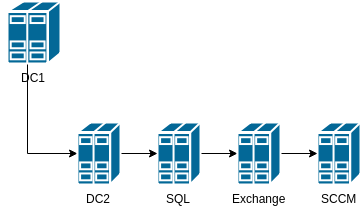
\includegraphics[width=8cm]{Netwerkdiagram.png}
\end{center}

\section{Server Requirements}

\begin{enumerate}
\item DC1
    \begin{enumerate}
    \item RAM: 2048 MB
    \item HDD: 50 GB
    \item Netwerkadapters: NAT en Internal Network (jenduf.gent)
            \begin{enumerate}
            \item NAT
            \end{enumerate}
            \begin{enumerate}
            \item IP: 192.168.1.1
            \item SN: 255.255.255.0
            \end{enumerate}
    \item OS Version: Windows Server 2016 
    \end{enumerate}
    
\clearpage

\item DC2
    \begin{enumerate}
    \item RAM: 2048 MB
    \item HDD: 50 GB
    \item Netwerkadapters: Internal Network (jenduf.gent)
            \begin{enumerate}
            \item IP: 192.168.1.2
            \item SN: 255.255.255.0
            \item DG: 192.168.1.1
            \end{enumerate}
    \item OS Version: Windows Server 2016 
    \end{enumerate}
    
\item SQL Server
    \begin{enumerate}
    \item RAM: 2048 MB
    \item HDD: 50 GB
    \item Netwerkadapters: Internal Network (jenduf.gent)
            \begin{enumerate}
            \item IP: 192.168.1.3
            \item SN: 255.255.255.0
            \item DG: 192.168.1.1
            \end{enumerate}
    \item OS Version: Windows Server 2016
    \item SQL Version: SQL Server 2013-2016
    \end{enumerate}
\item Exchange Server
    \begin{enumerate}
    \item RAM: 8096 MB
    \item HDD: 100 GB
    \item Netwerkadapters: Internal Network (jenduf.gent)
            \begin{enumerate}
            \item IP: 192.168.1.4
            \item SN: 255.255.255.0
            \item DG: 192.168.1.1
            \end{enumerate}
    \item OS Version: Windows Server 2016
    \item Exchange Version: Exchange Server 2013-2016
    \end{enumerate}
\item SCCM Server
    \begin{enumerate}
    \item RAM: 8089 MB
    \item HDD: 100 GB
    \item Netwerkadapters: Internal Network (jenduf.gent)
            \begin{enumerate}
            \item IP: 192.168.1.5
            \item SN: 255.255.255.0
            \item DG: 192.168.1.1
            \end{enumerate}
    \item OS Version: Windows Server 2016
    \item OS Version: Windows Deployment Server 2012
    \end{enumerate}
\end{enumerate}

\section{Windows Server Installatie}
\begin{center}
	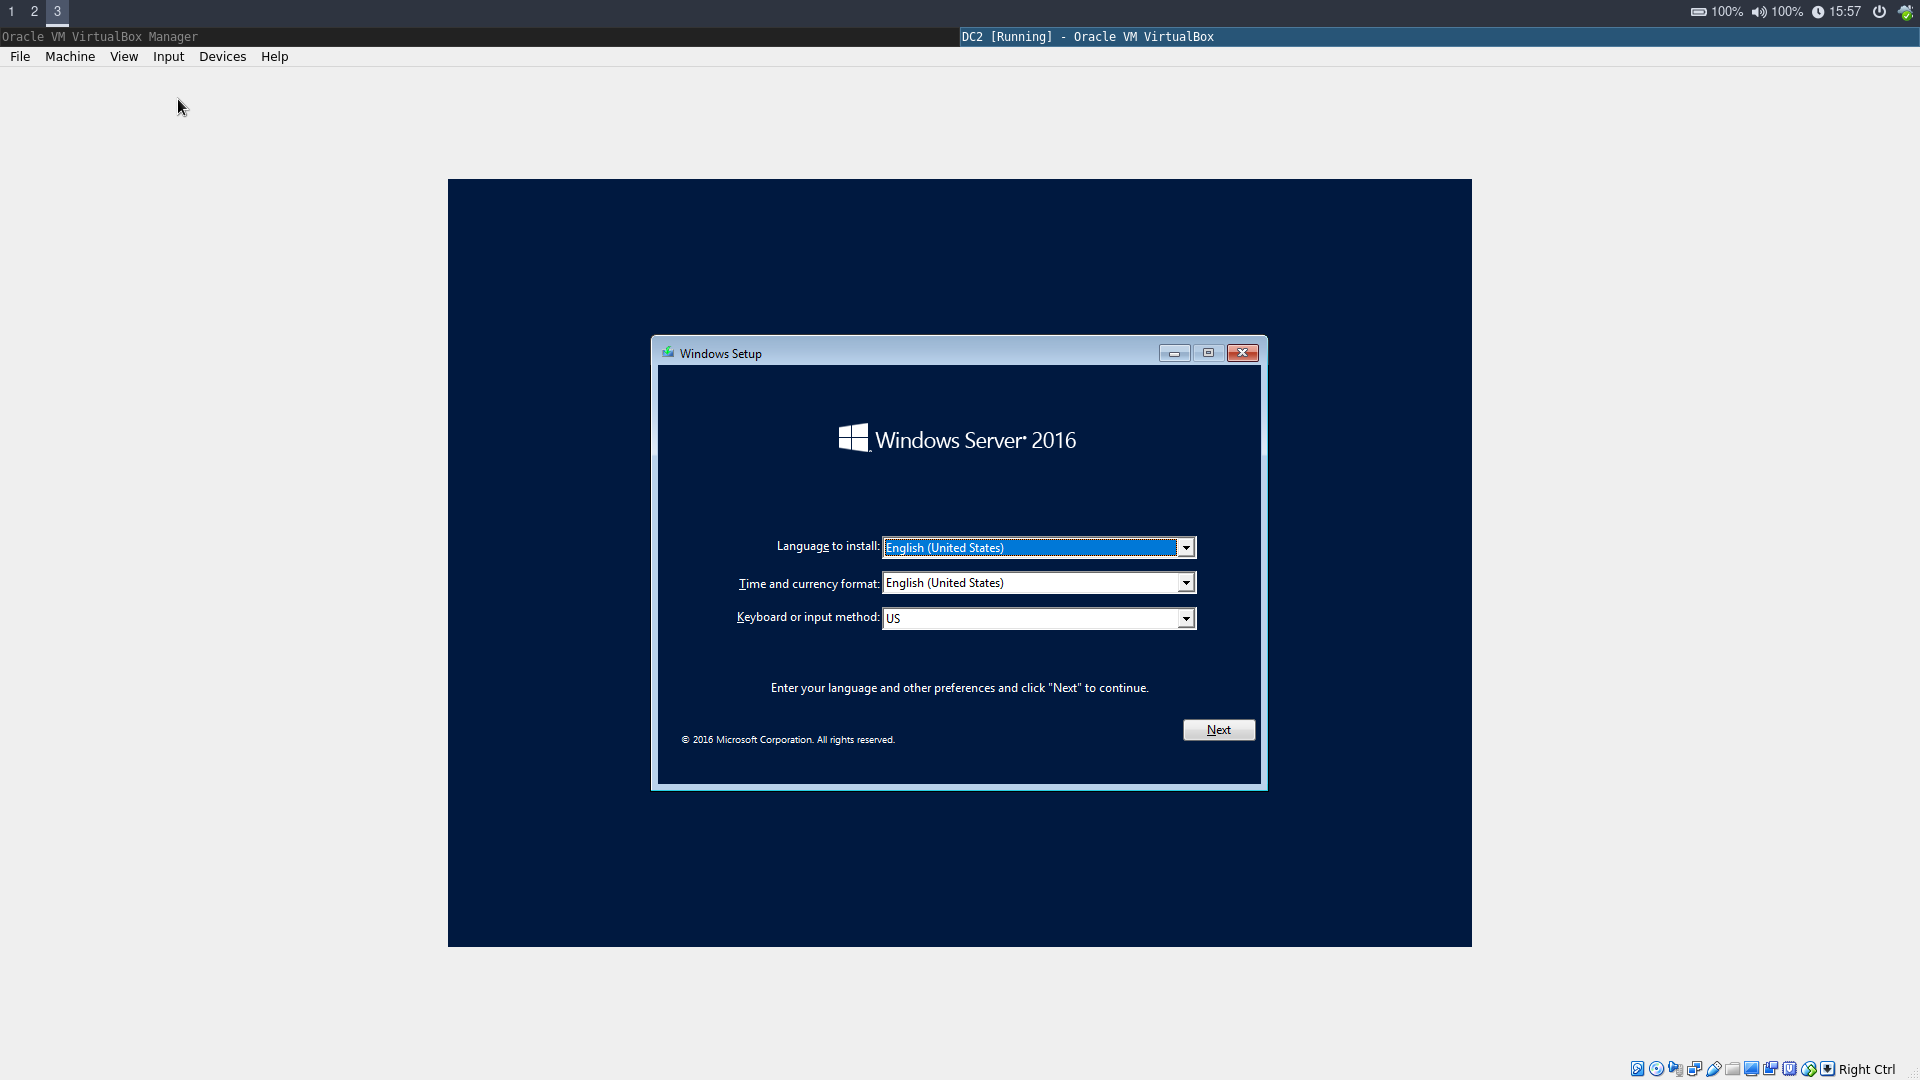
\includegraphics[width=15cm]{Pictures/Windows_Install/1542293852.png}
	Selecteer de gewenste taalinstellingen.
\end{center}
\begin{center}
	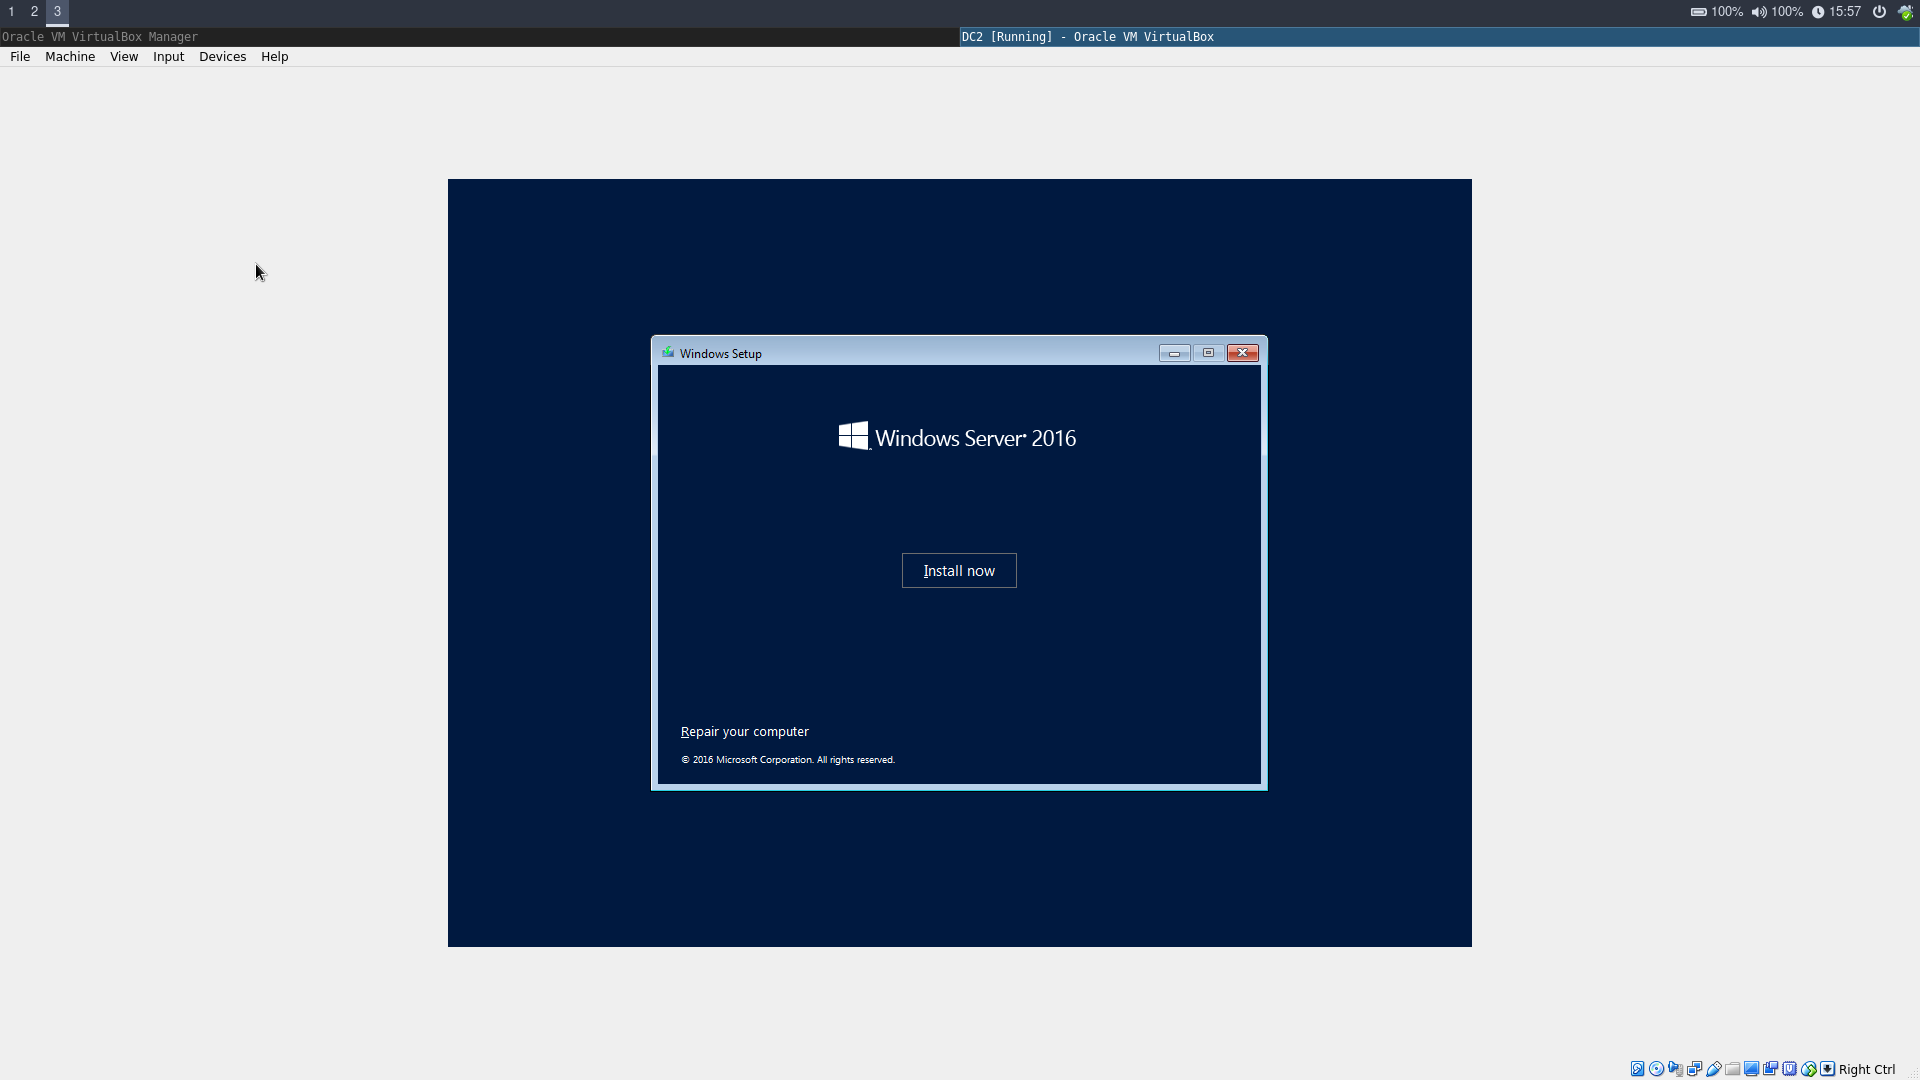
\includegraphics[width=15cm]{Pictures/Windows_Install/1542293872.png}
	
	Start de installatie.
\end{center}
\begin{center}
	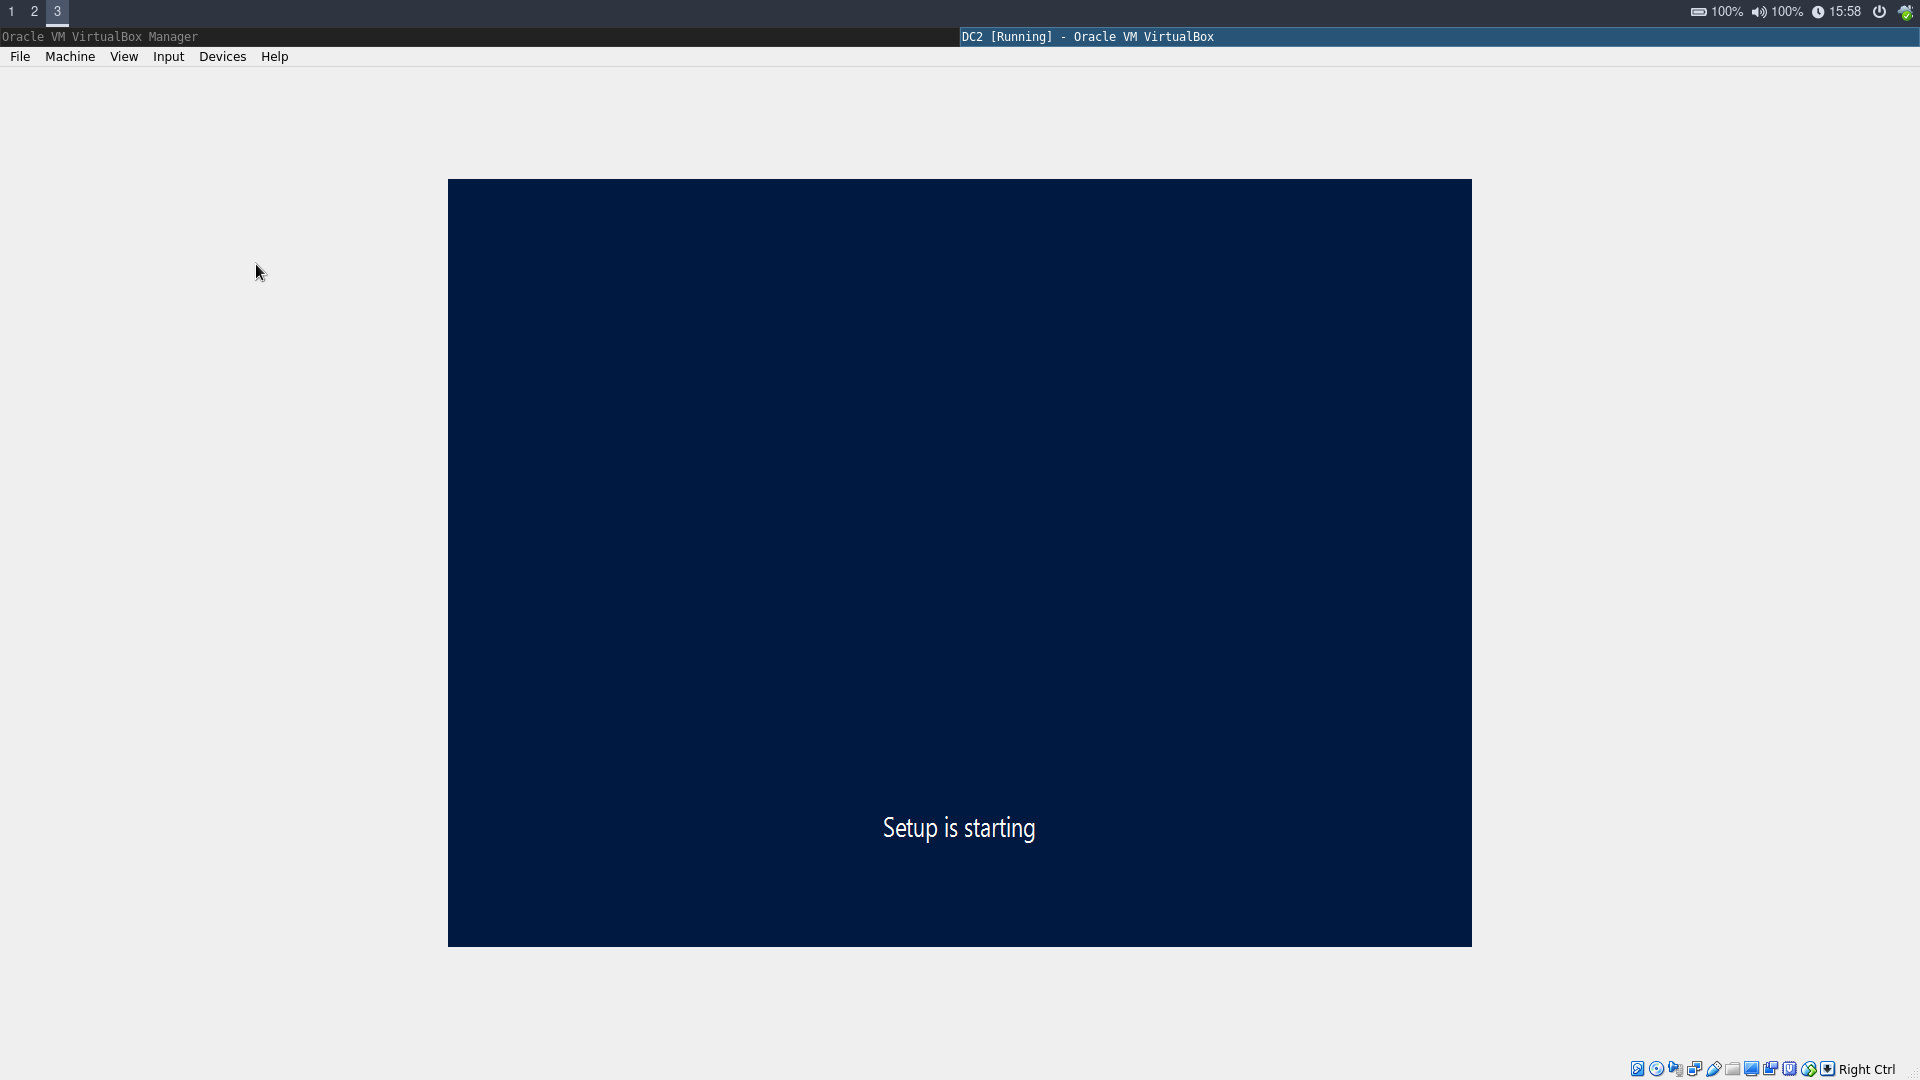
\includegraphics[width=15cm]{Pictures/Windows_Install/1542293887.png}
\end{center}
\begin{center}
	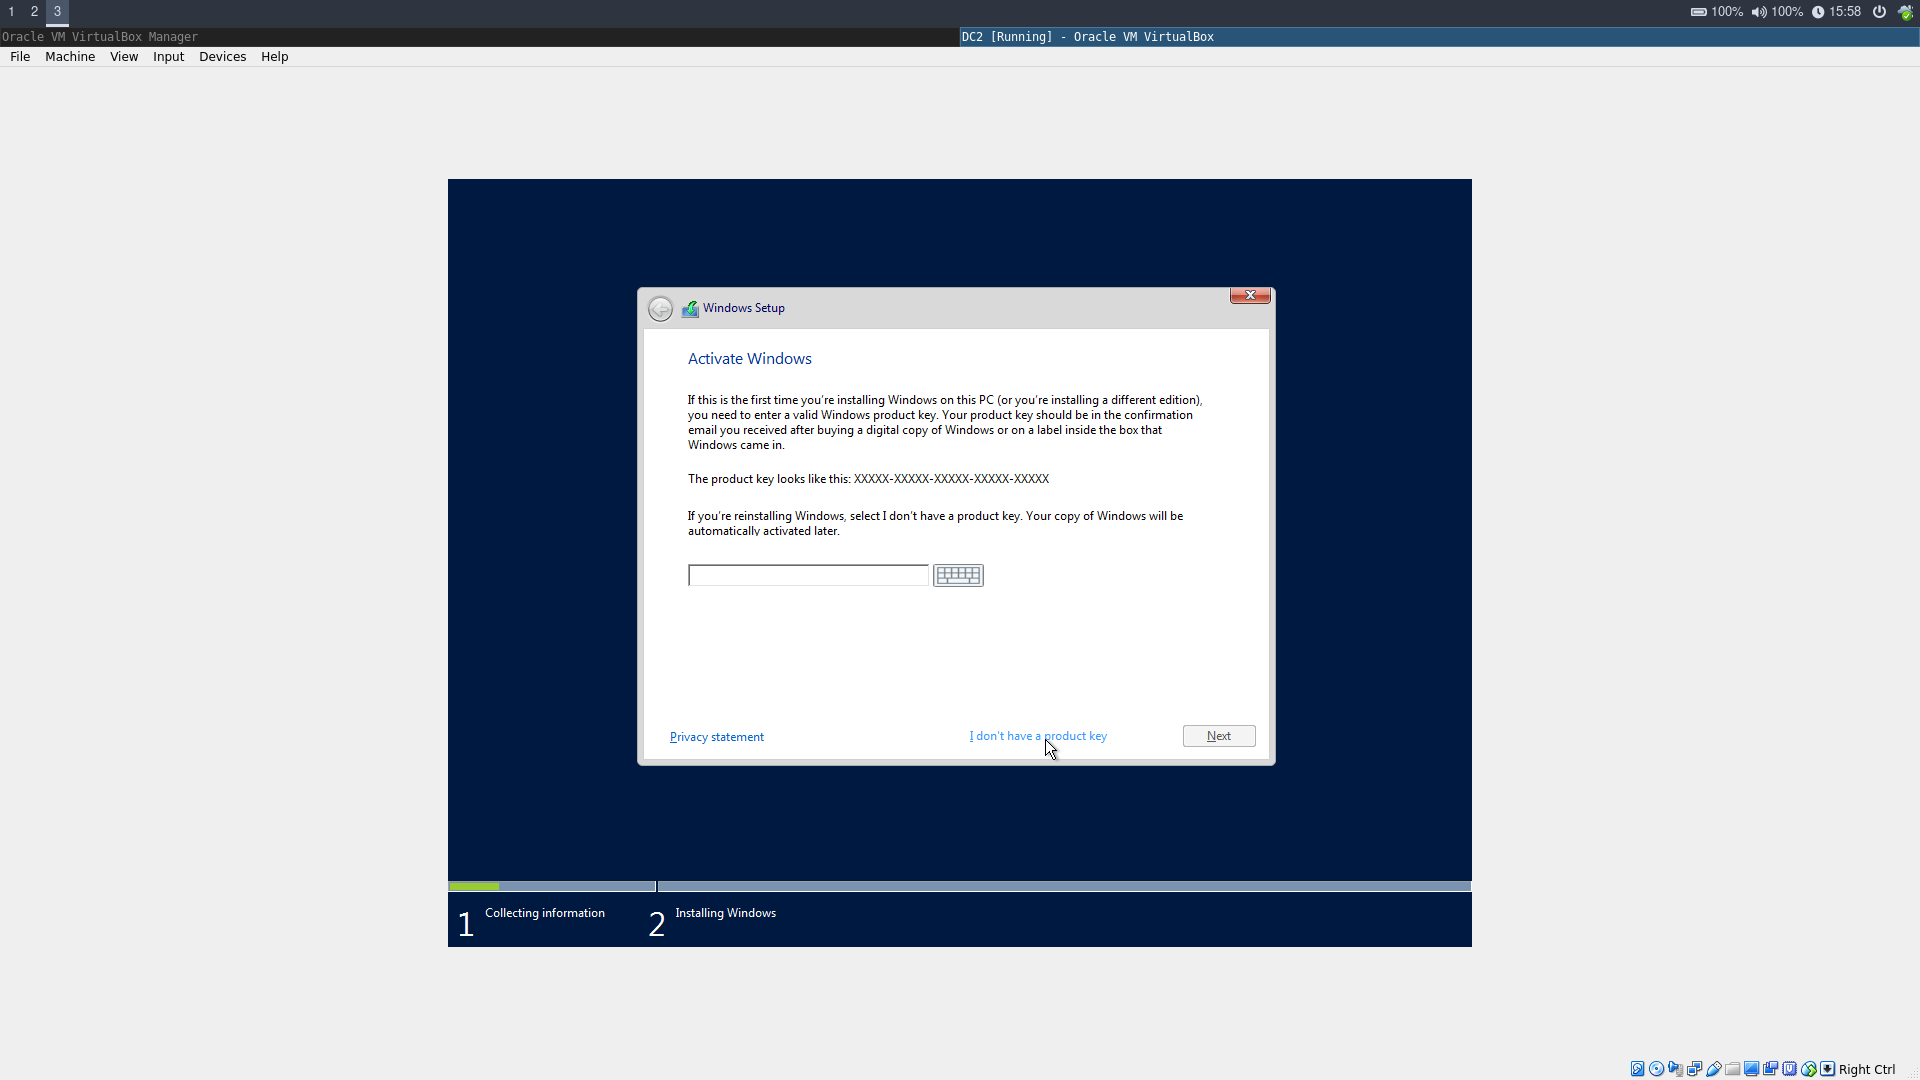
\includegraphics[width=15cm]{Pictures/Windows_Install/1542293899.png}
	
	Selecteer "I don't have a product key".
\end{center}
\begin{center}
	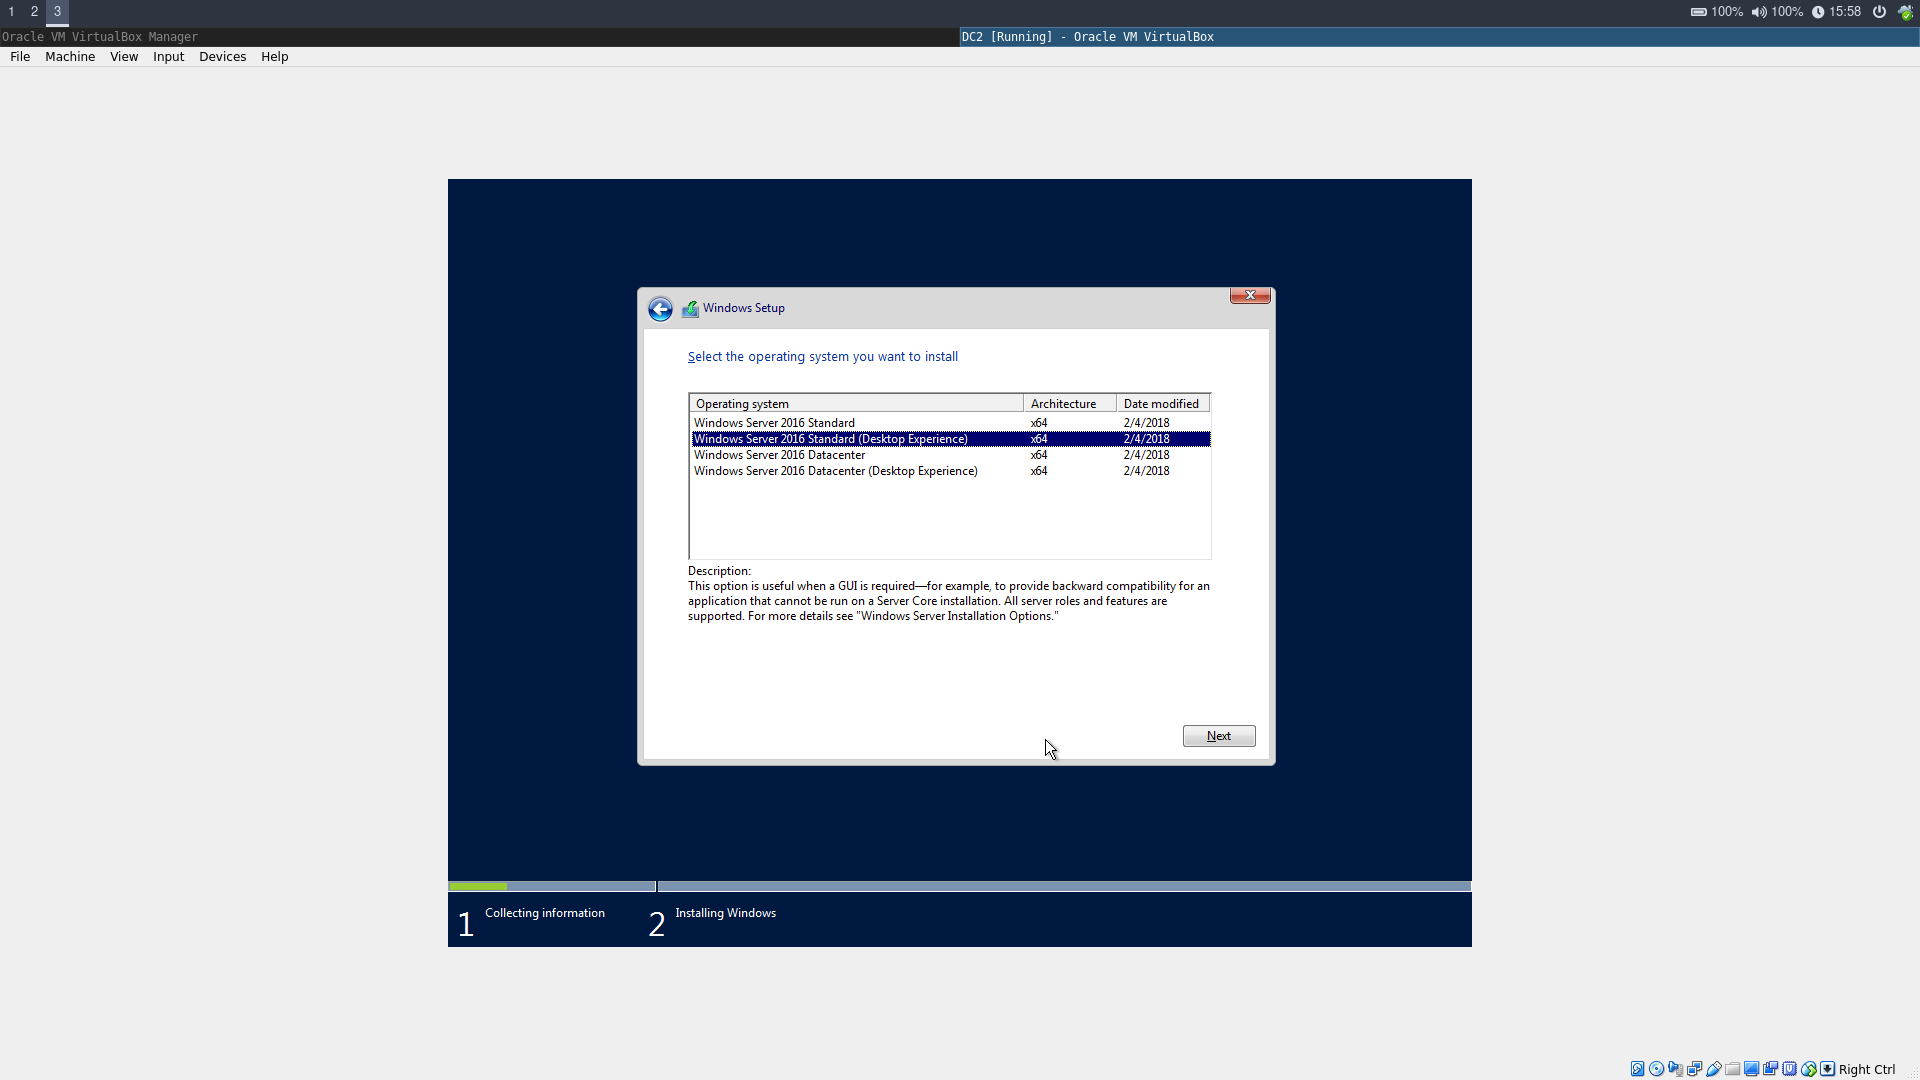
\includegraphics[width=15cm]{Pictures/Windows_Install/1542293908.png}
	
	Selecteer "Windows Server 2016 Standard (Desktop Experience)".
\end{center}
\begin{center}
	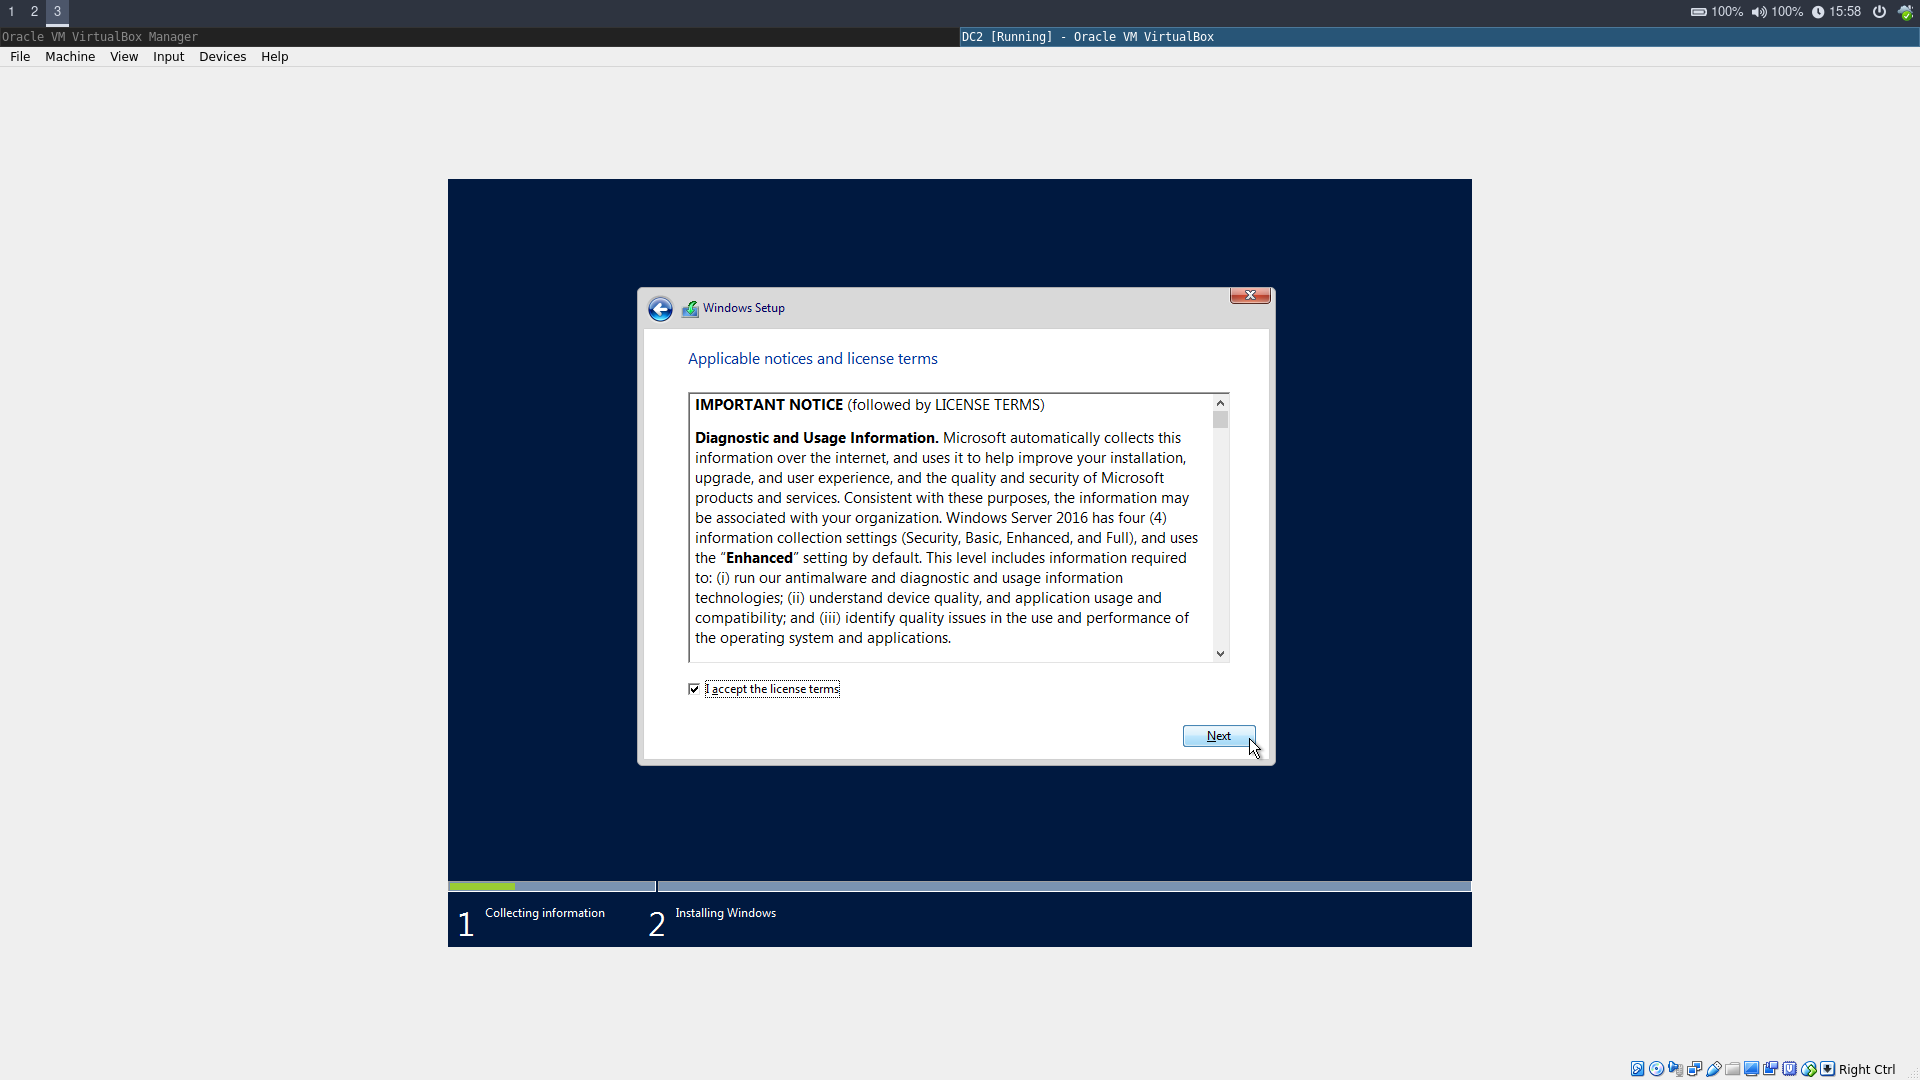
\includegraphics[width=15cm]{Pictures/Windows_Install/1542293921.png}
	
	Ga akkoord met de gebruiksvoorwaarden.
\end{center}
\begin{center}
	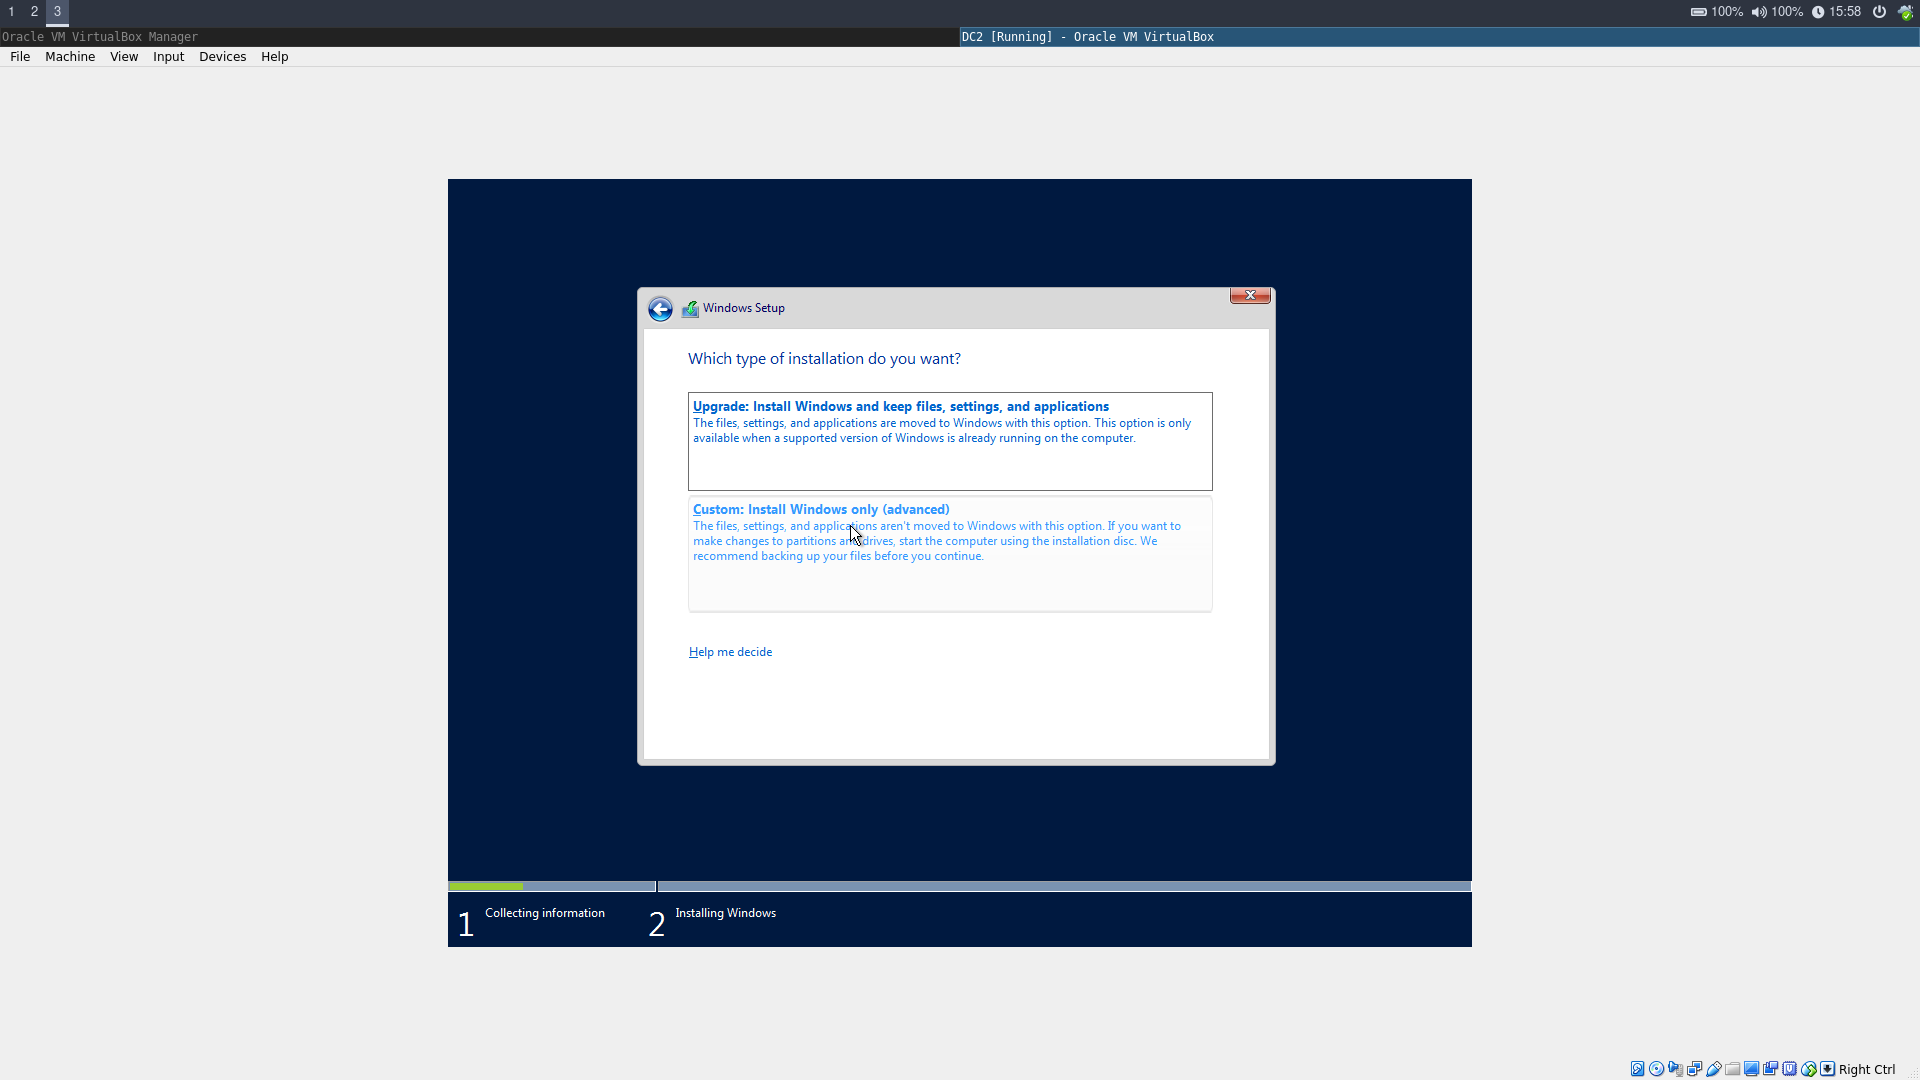
\includegraphics[width=15cm]{Pictures/Windows_Install/1542293929.png}
	
	Selecteer "Costum: Install Windows only (Advanced)".
\end{center}
\begin{center}
	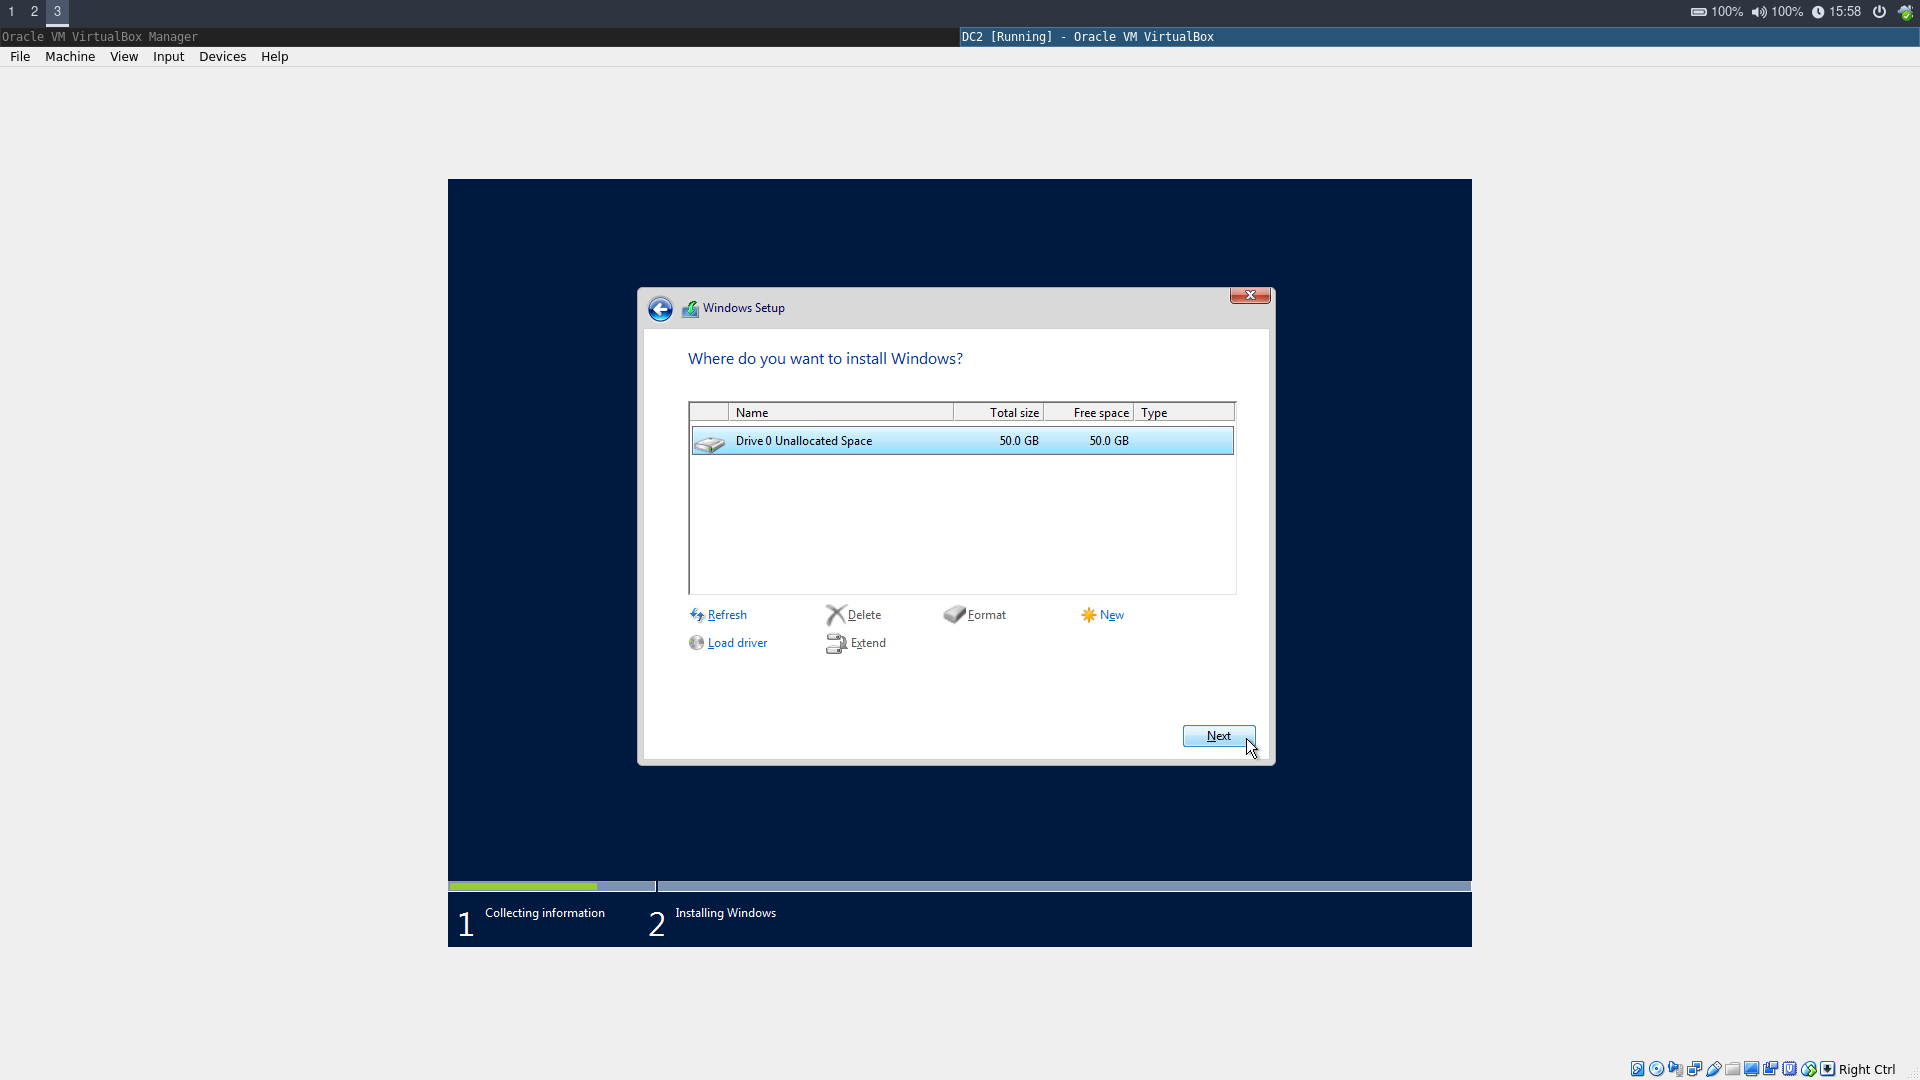
\includegraphics[width=15cm]{Pictures/Windows_Install/1542293934.png}
	
	Ga verder.
\end{center}
\begin{center}
	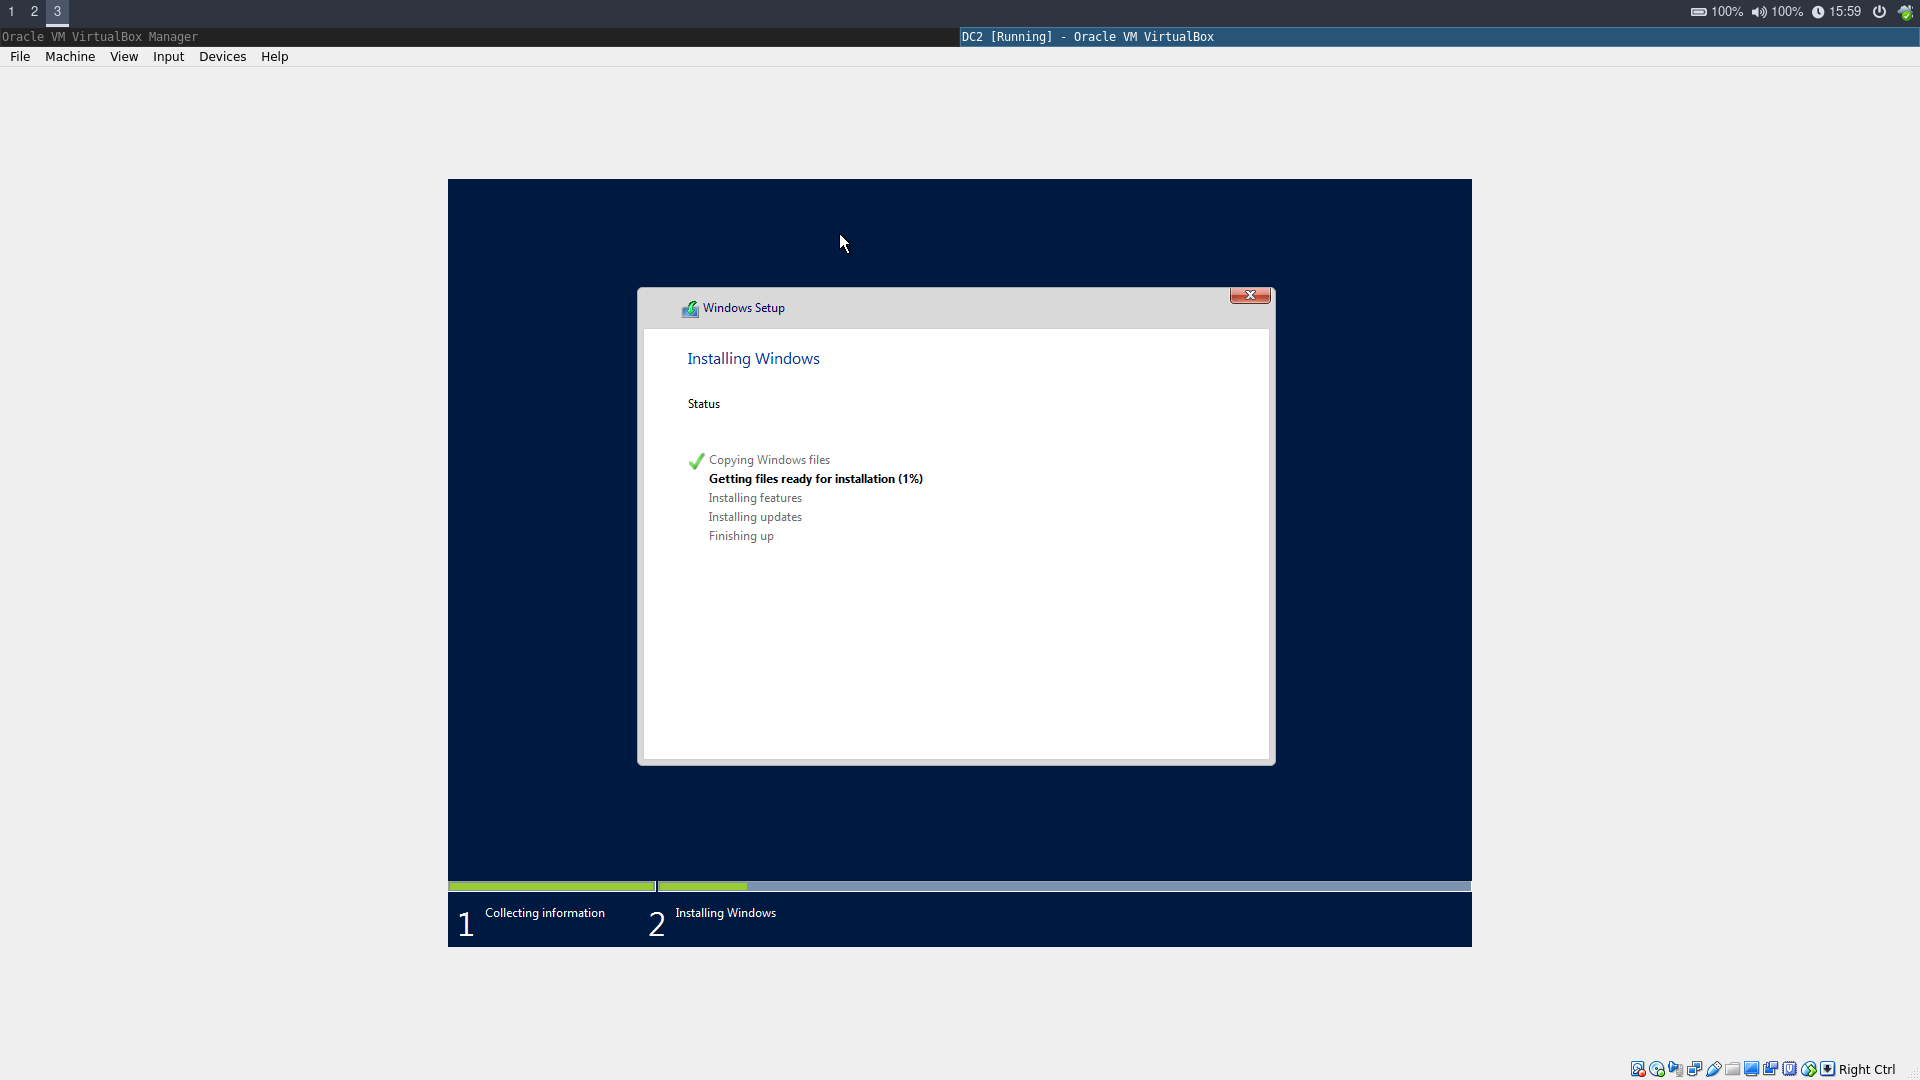
\includegraphics[width=15cm]{Pictures/Windows_Install/1542293945.png}
\end{center}
\subsection{Server Hernoemen}
\begin{center}
	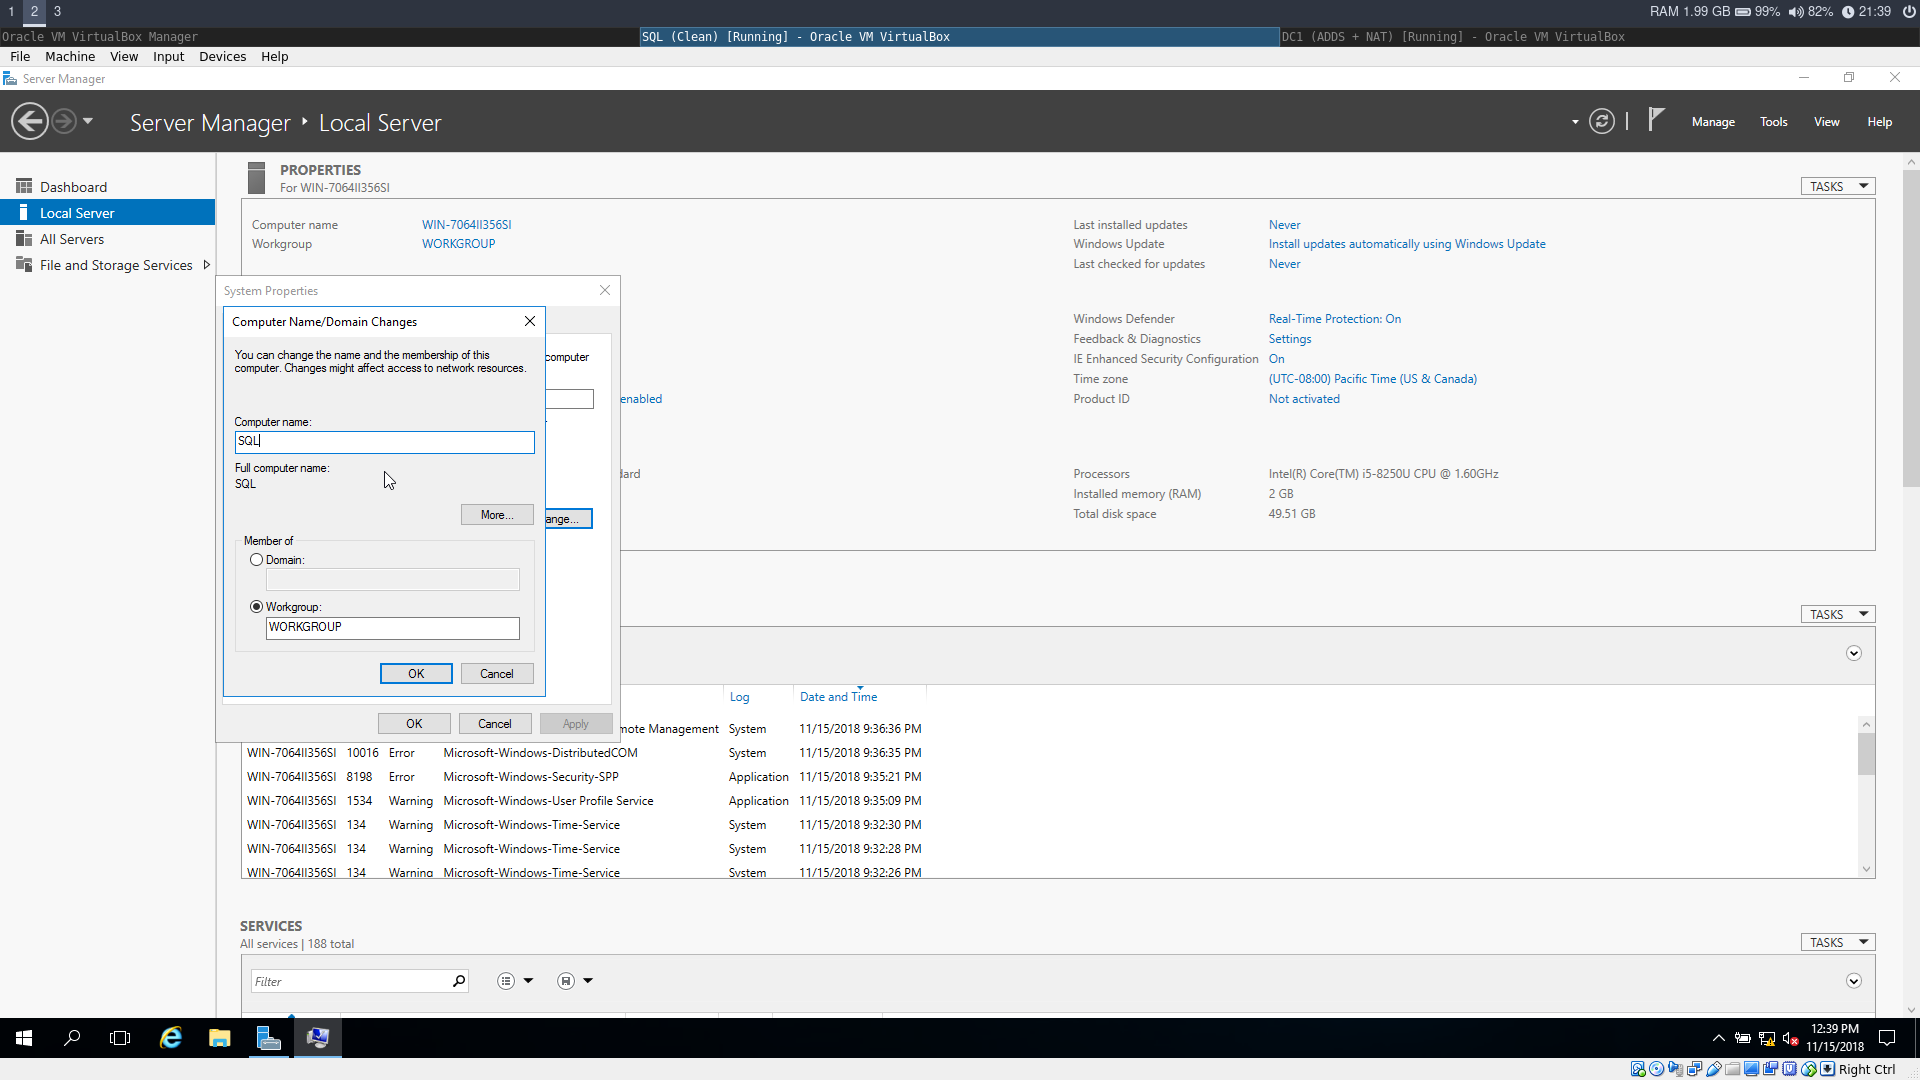
\includegraphics[width=15cm]{Pictures/SQL/1542314353.png}
\end{center}
\subsection{IP Instellingen}
\begin{center}
	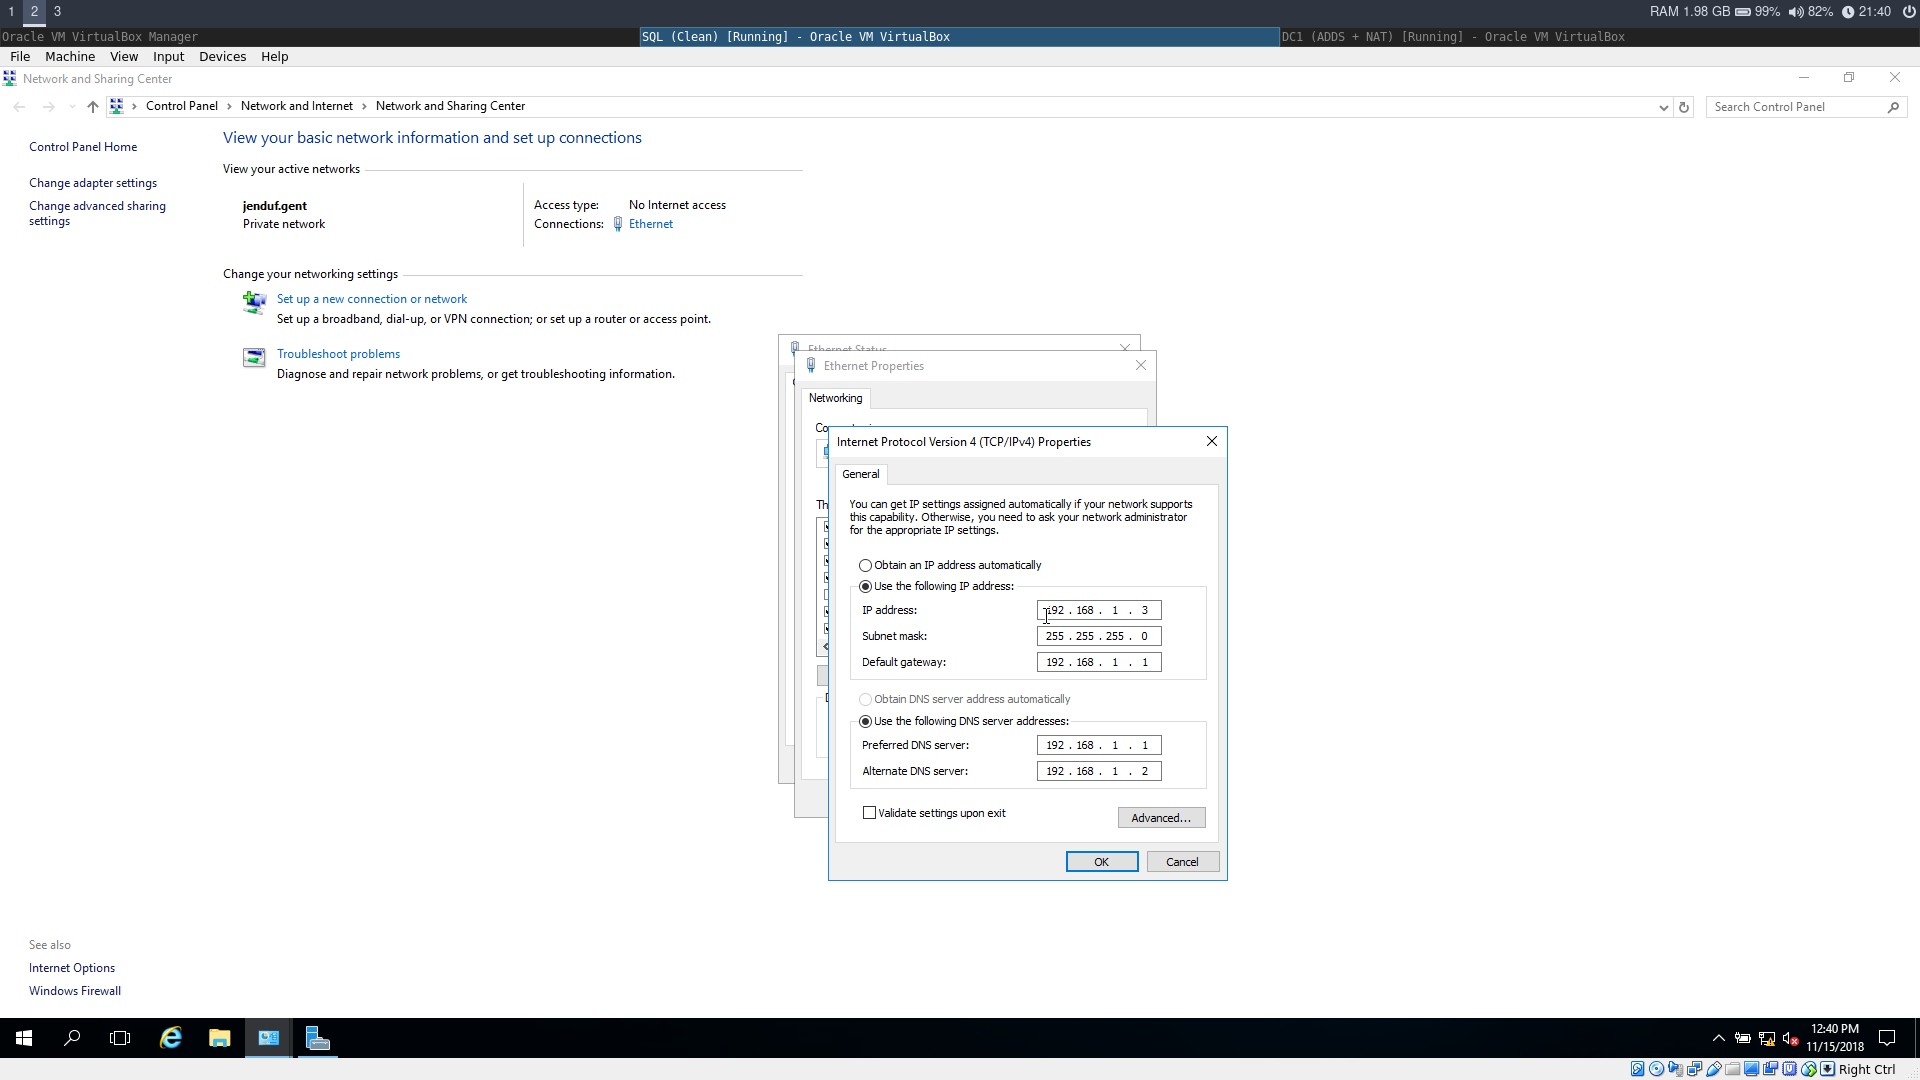
\includegraphics[width=15cm]{Pictures/SQL/1542314452.png}
\end{center}
\subsection{Toevoegen aan het domein}
\begin{center}
	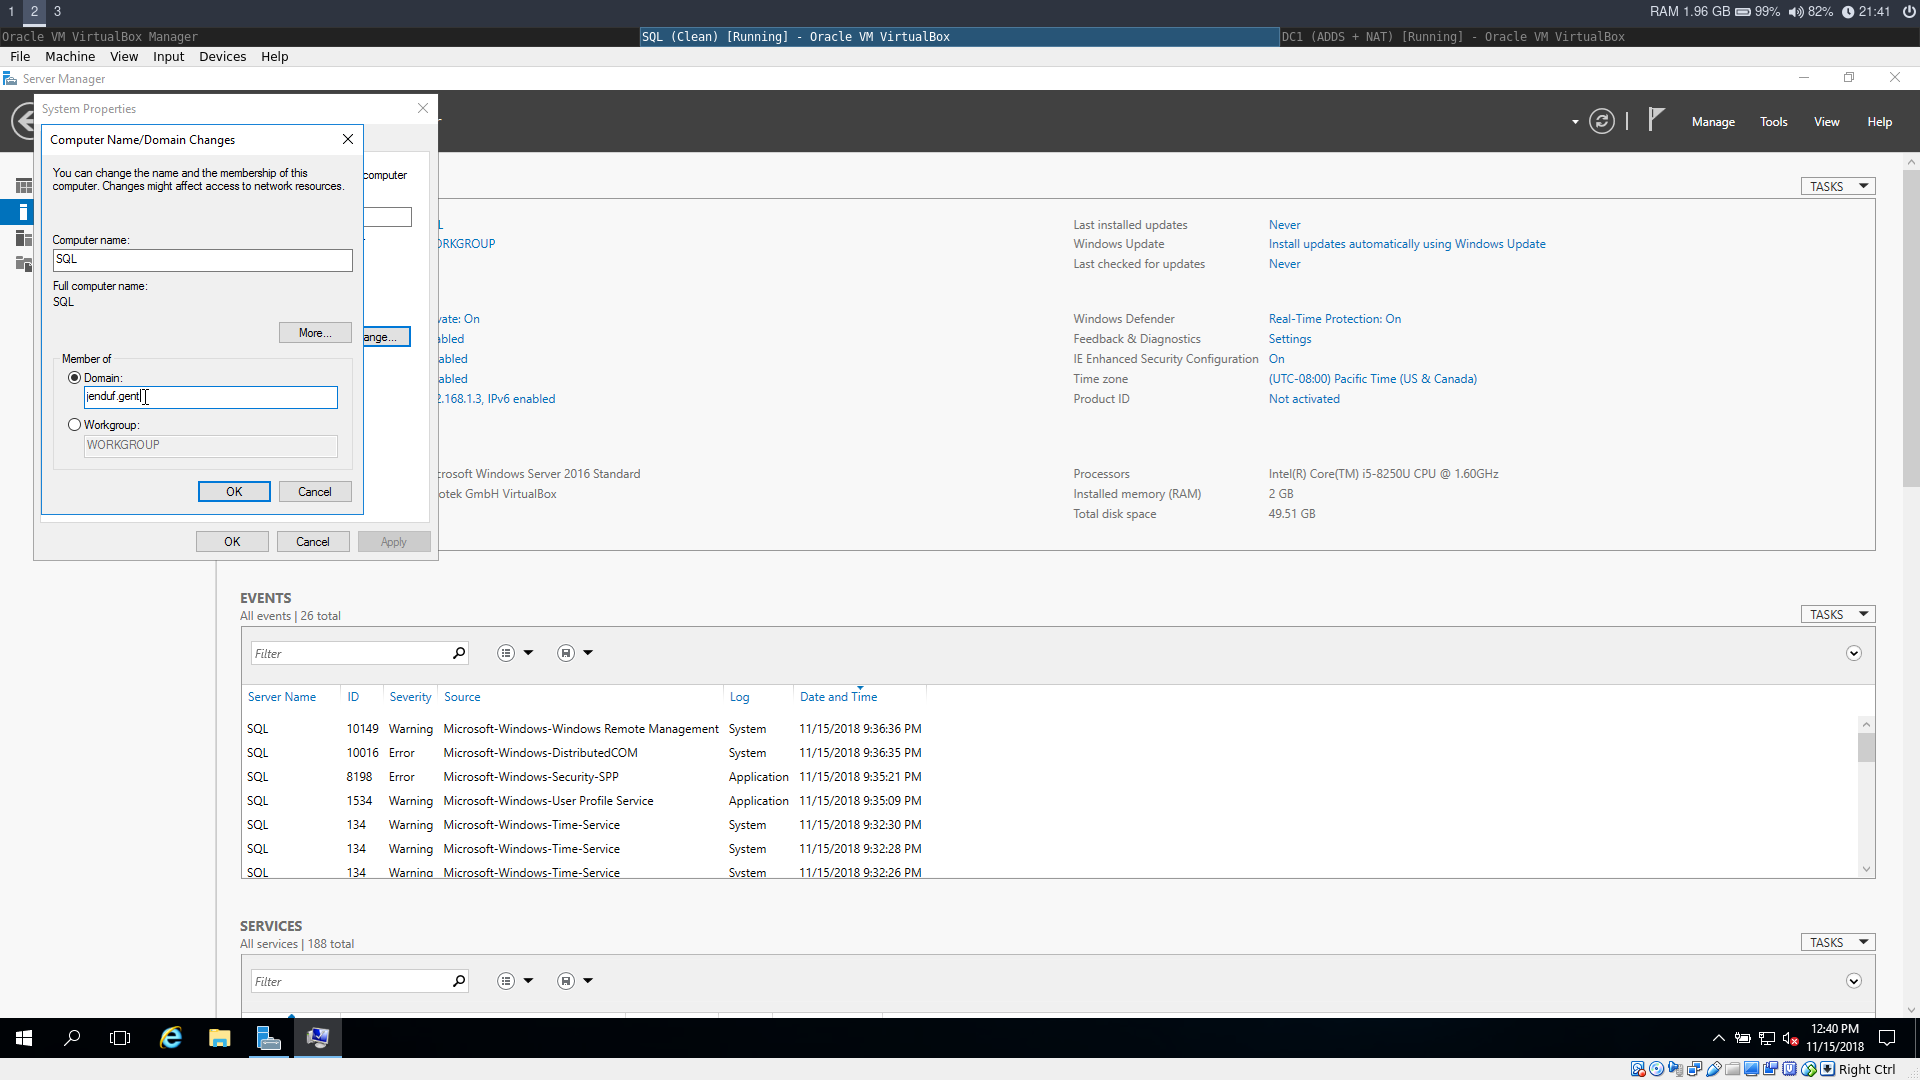
\includegraphics[width=15cm]{Pictures/SQL/1542314488.png}
	
	Geef als domein jenduf.gent in.
\end{center}
\begin{center}
	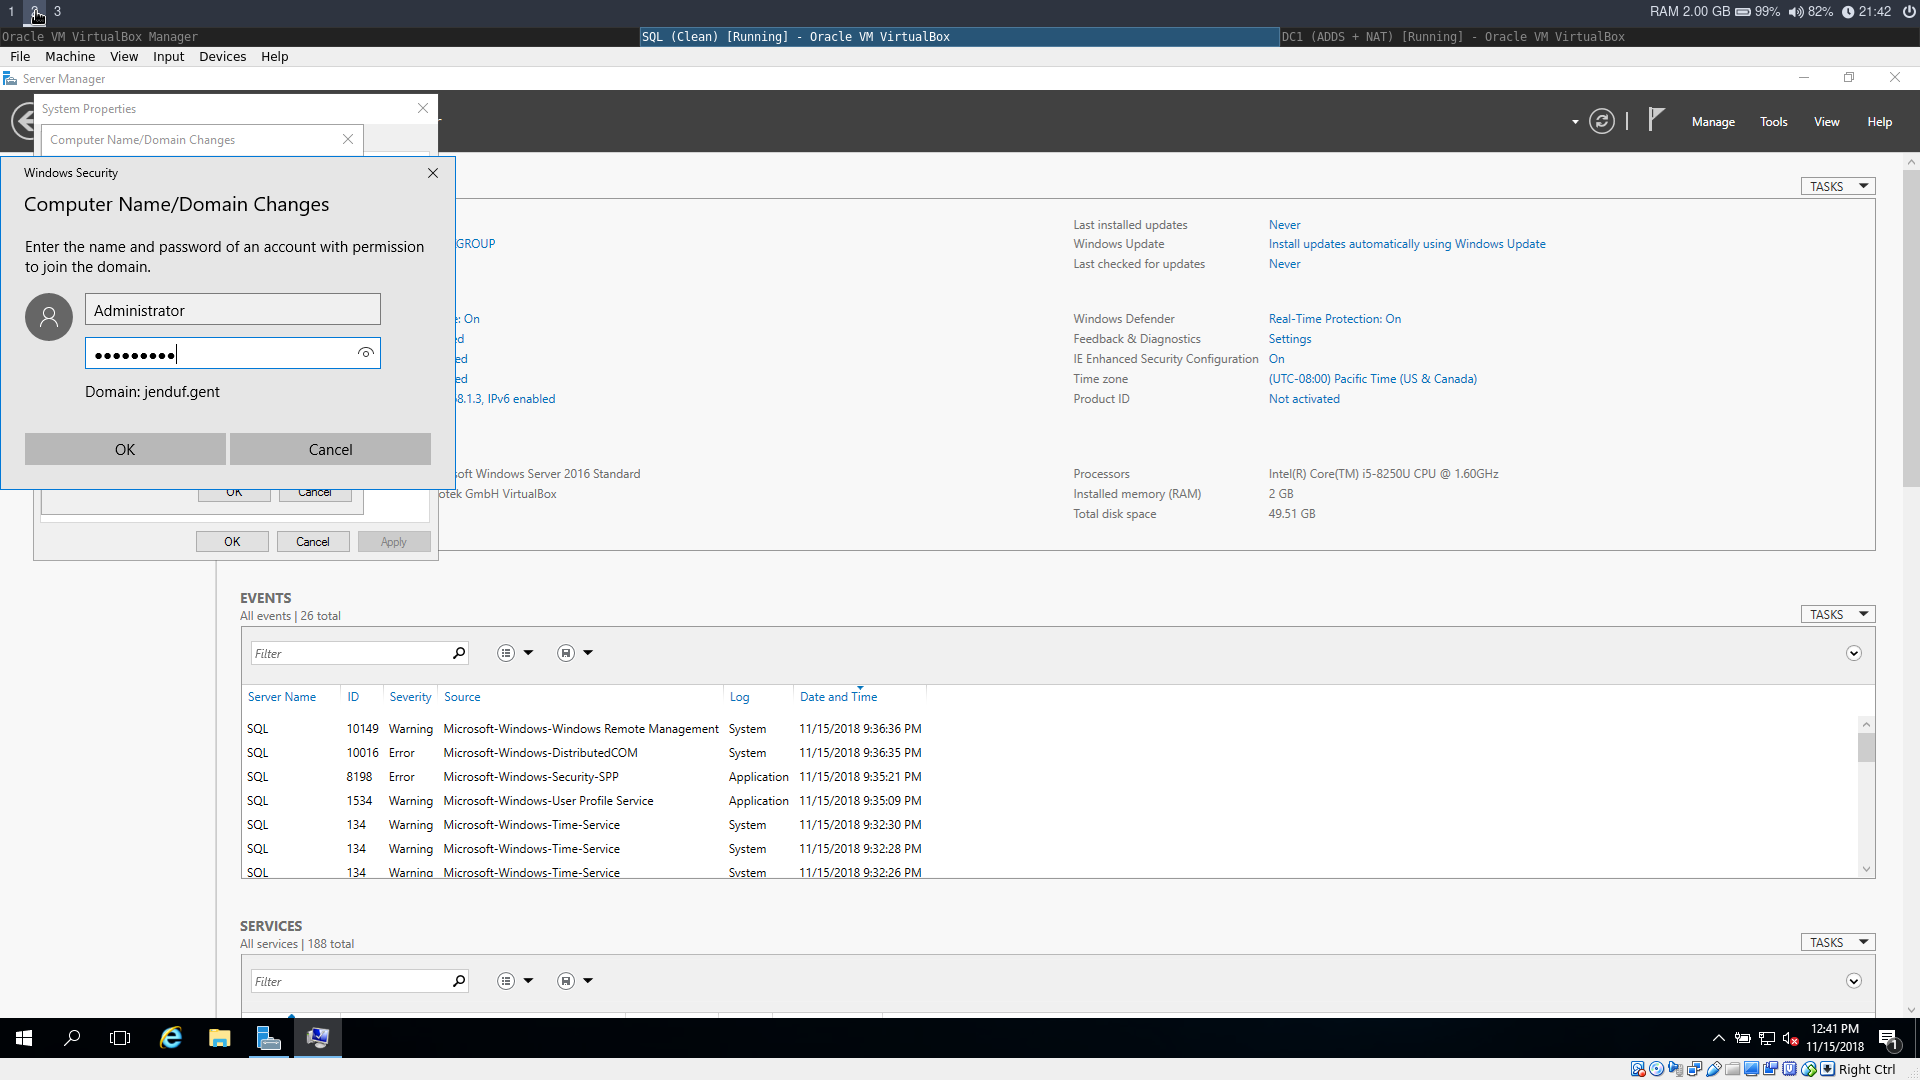
\includegraphics[width=15cm]{Pictures/SQL/1542314556.png}
	
	Geef gebruikersnaam "Administrator" in en paswoord "Admin2018".
\end{center}
\begin{center}
	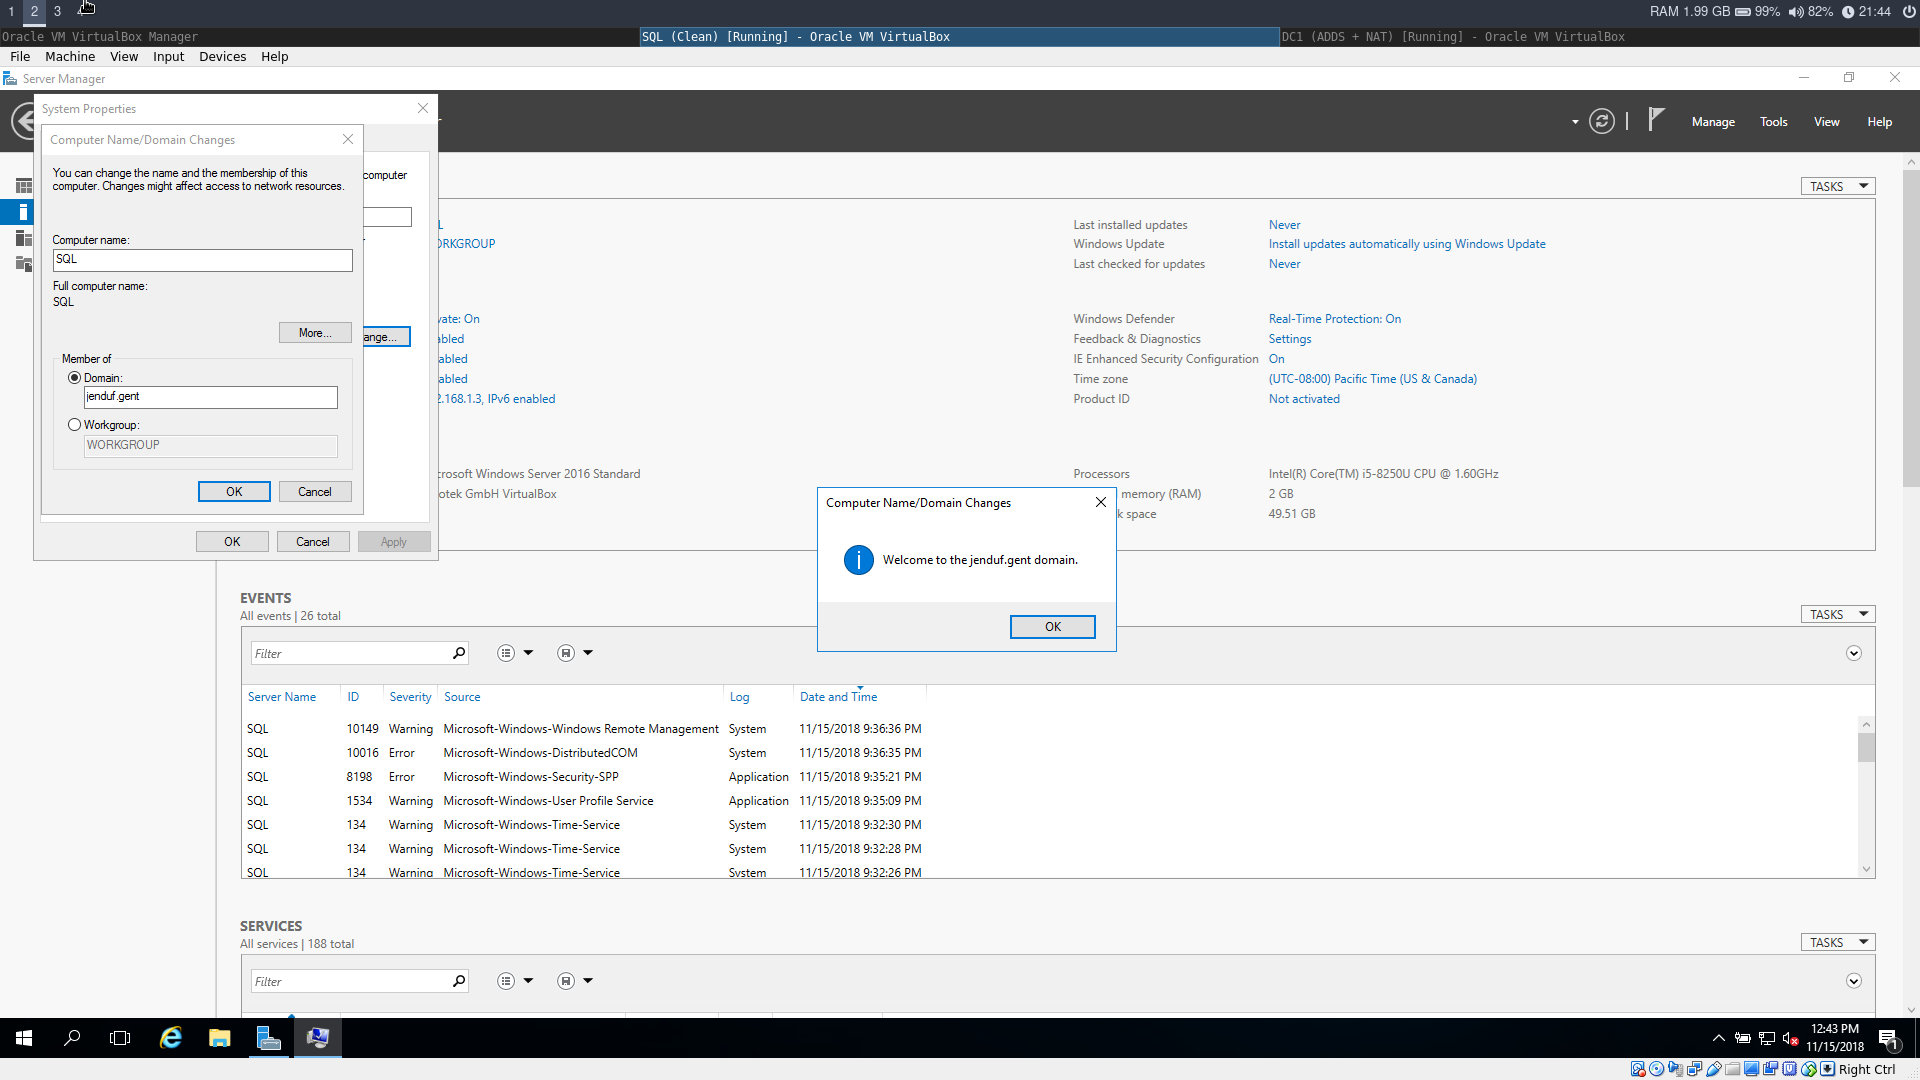
\includegraphics[width=15cm]{Pictures/SQL/1542314682.png}
	
	De connectie is geslaagd bij het weergeven van volgende boodschap.
\end{center}

\clearpage

\section{Installatie SQL Server}
	
\begin{center}
	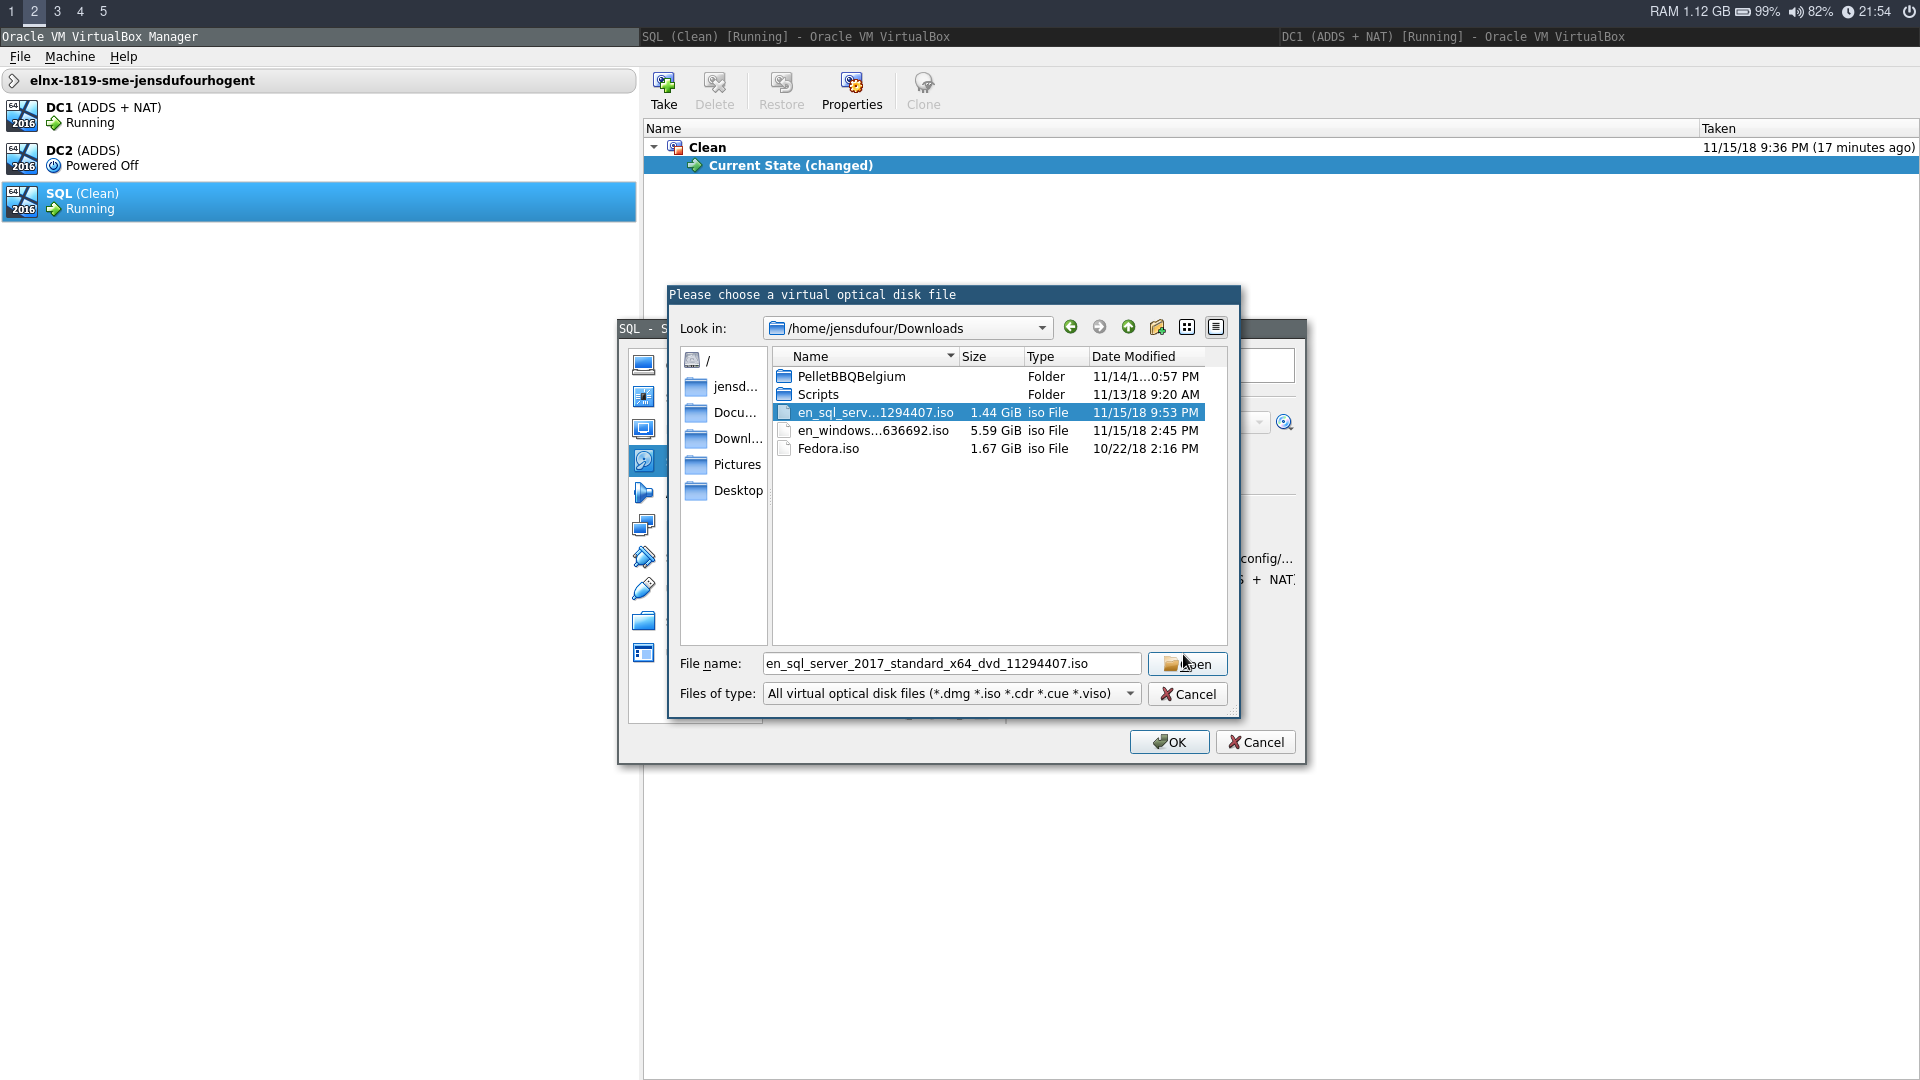
\includegraphics[width=15cm]{Pictures/SQL/1542315276.png}
	
	Verbind de installatieschijf van SQL Server met de VM.
\end{center}
\begin{center}
	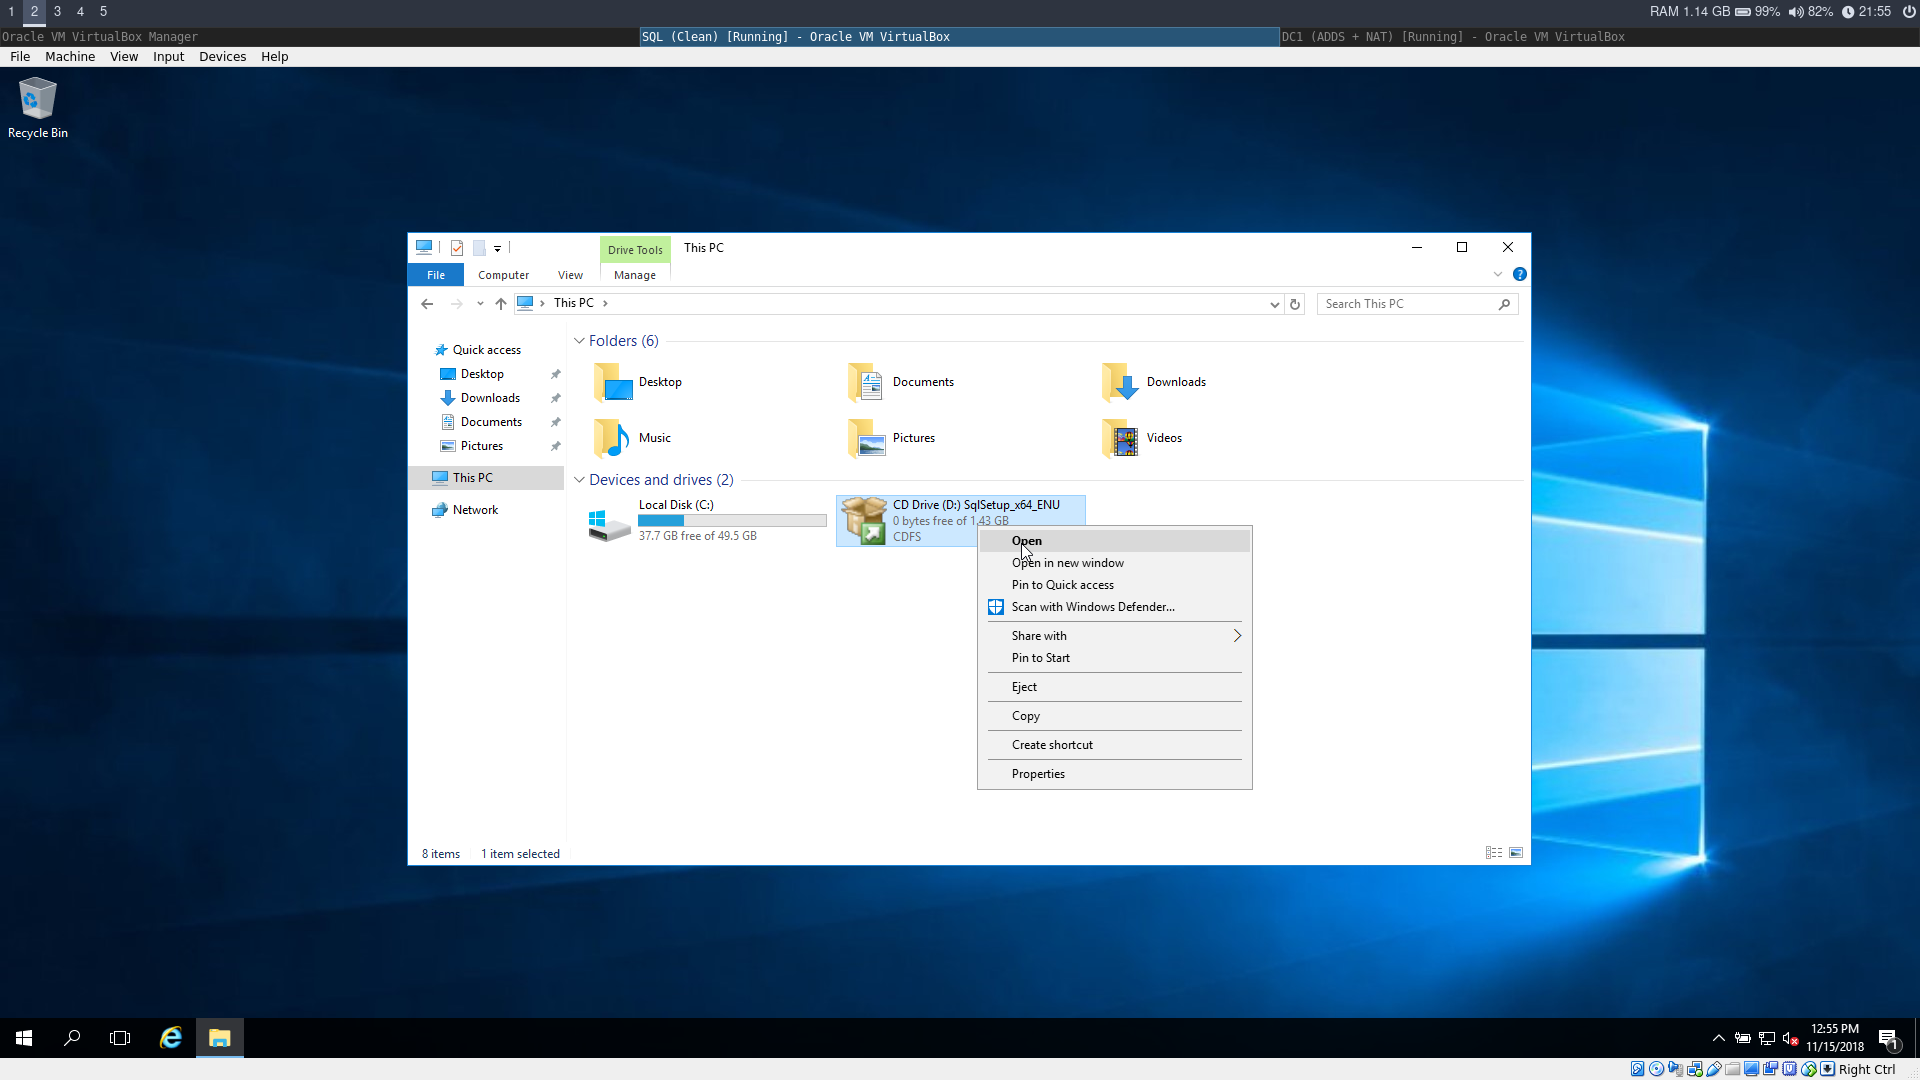
\includegraphics[width=15cm]{Pictures/SQL/1542315338.png}
	
	Start de installatieprocedure vanuit Windows Verkenner.
\end{center}
\begin{center}
	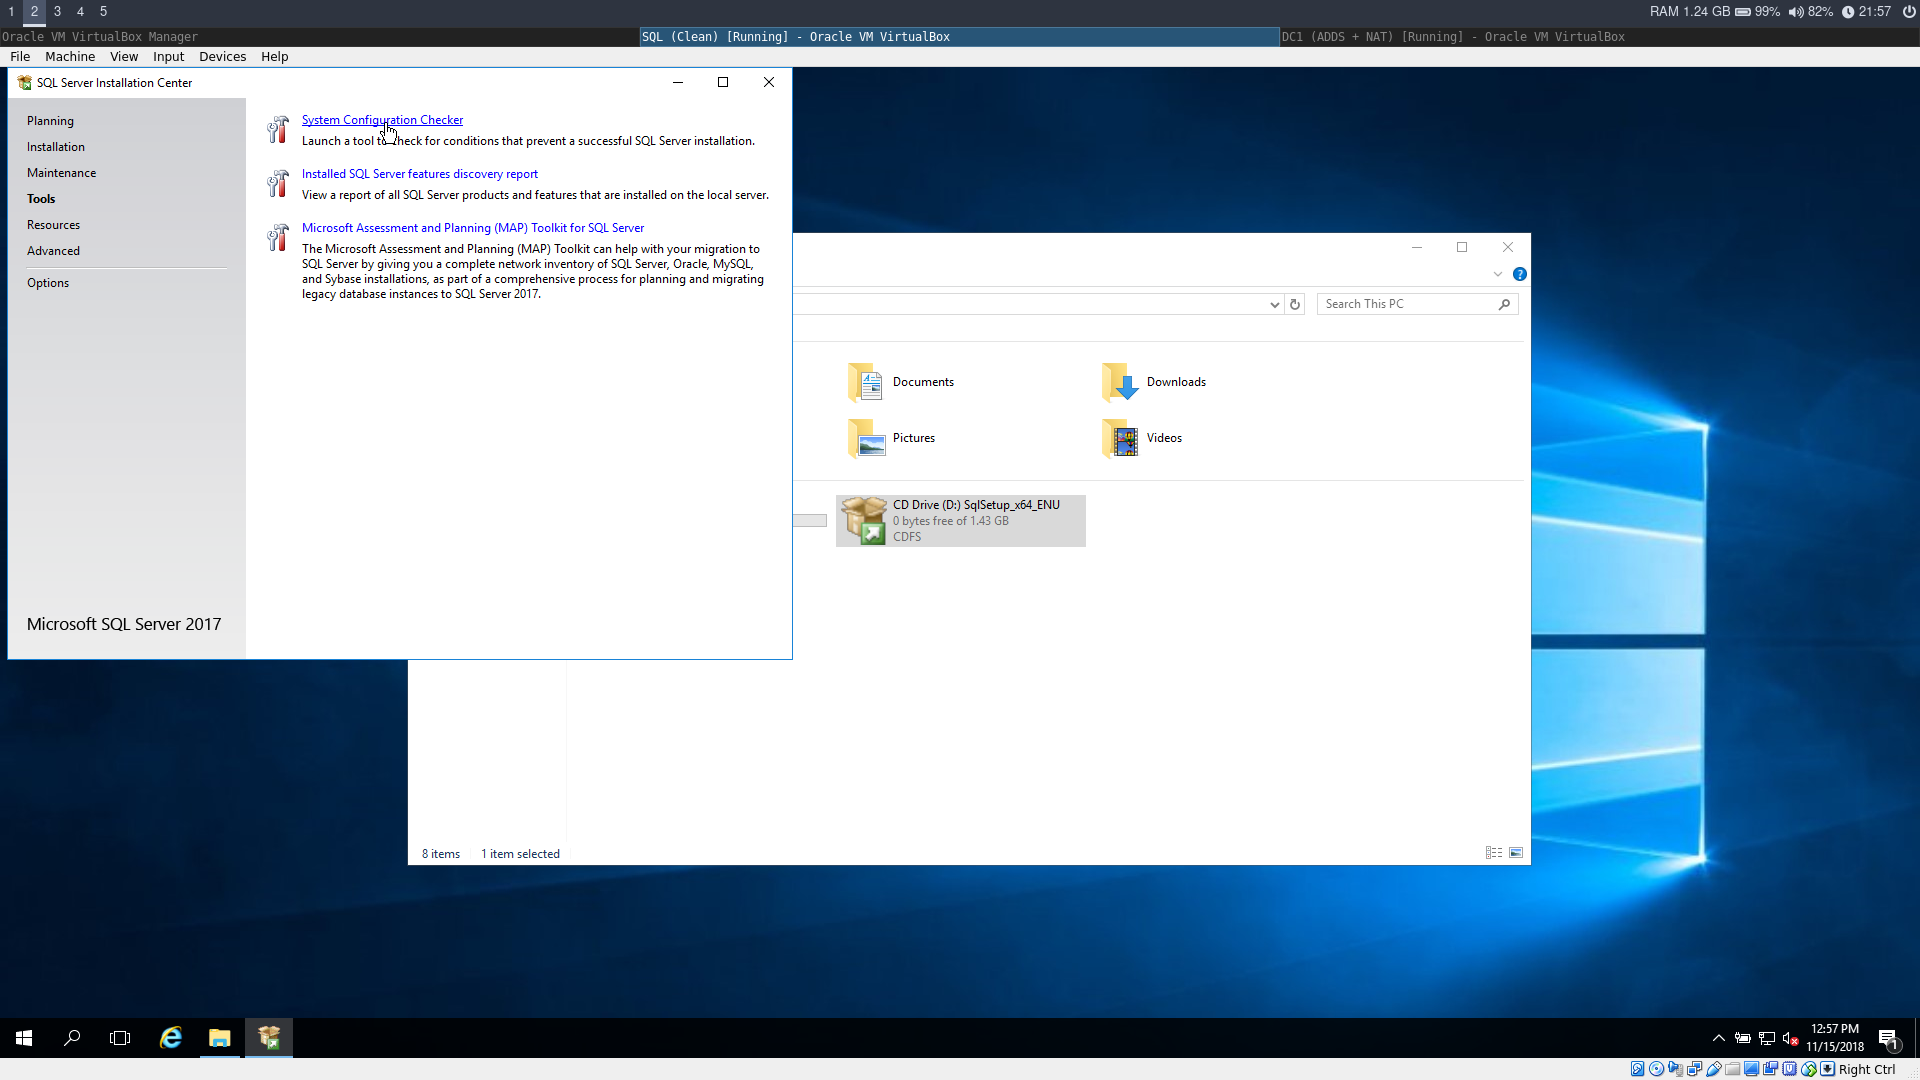
\includegraphics[width=15cm]{Pictures/SQL/1542315421.png}
	
	Voer de systeemsconfiguratietesten uit.
\end{center}
\begin{center}
	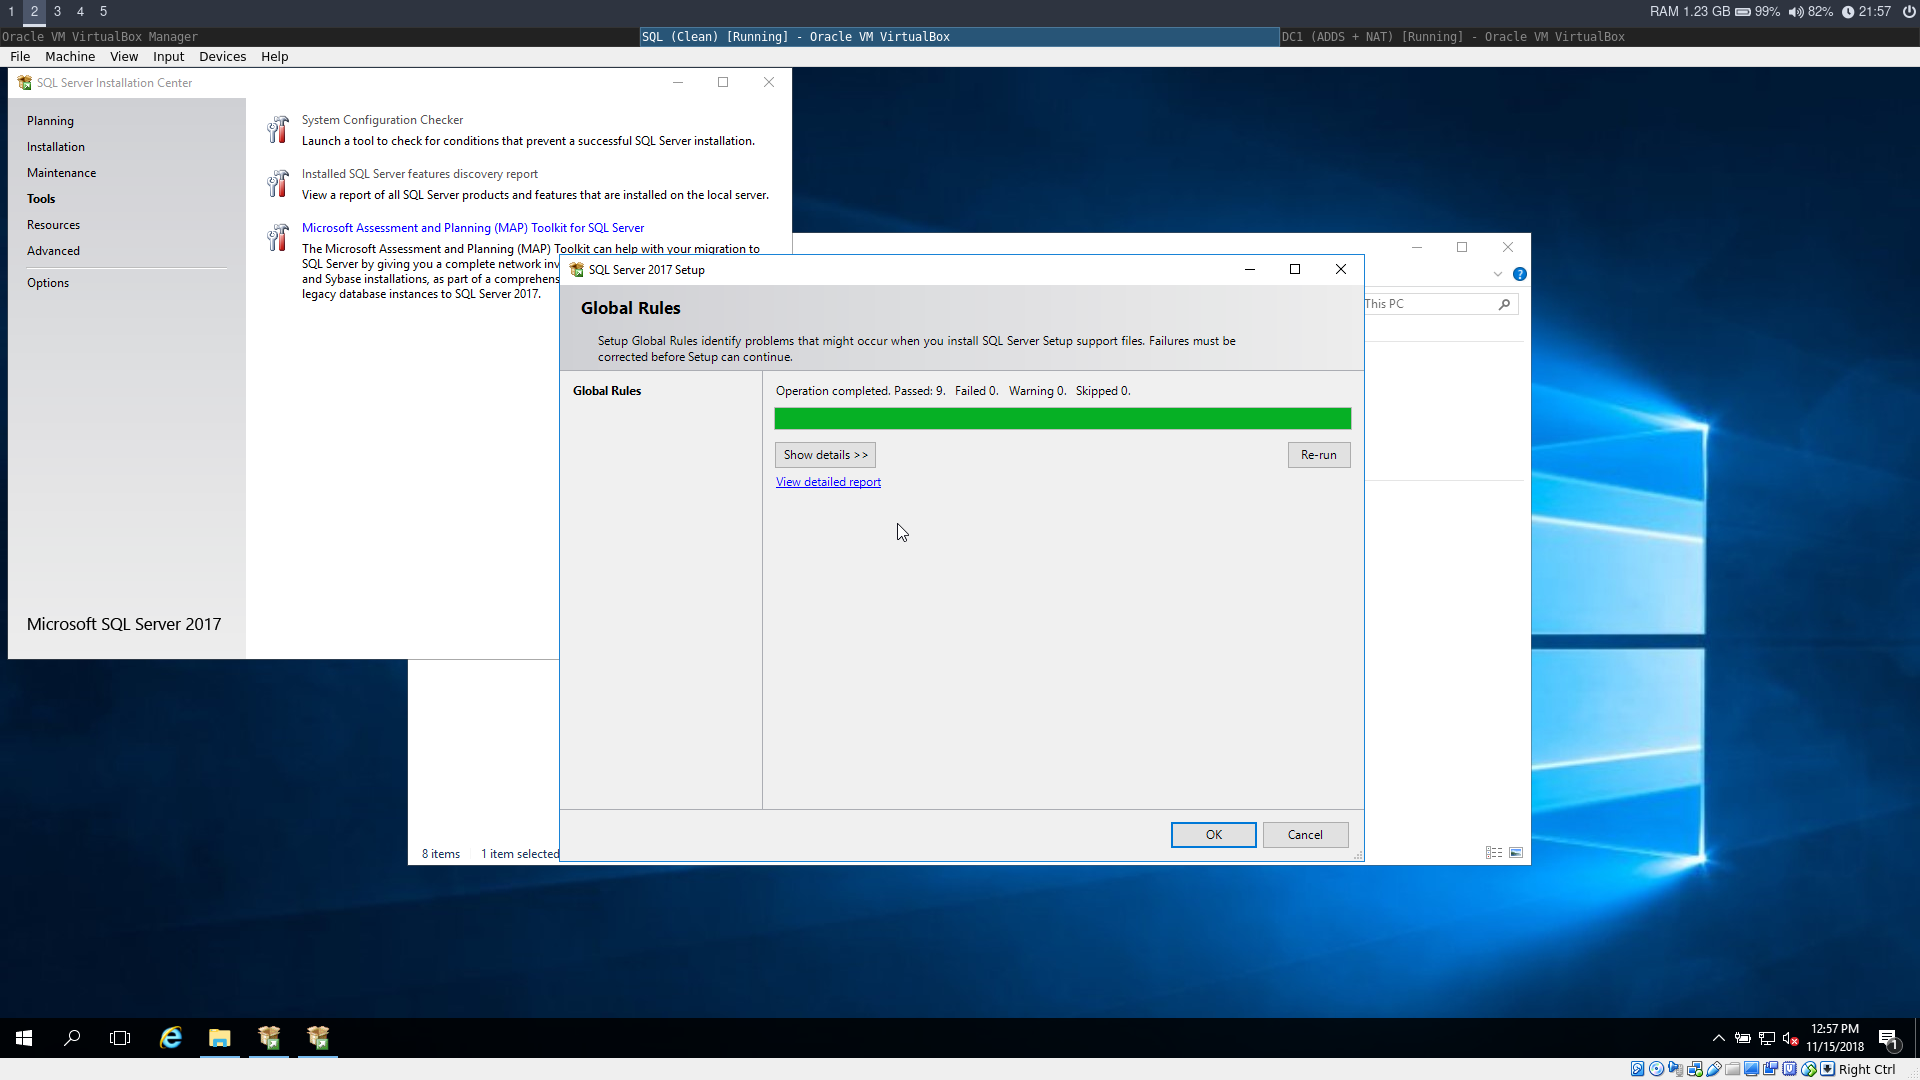
\includegraphics[width=15cm]{Pictures/SQL/1542315456.png}
\end{center}
\begin{center}
	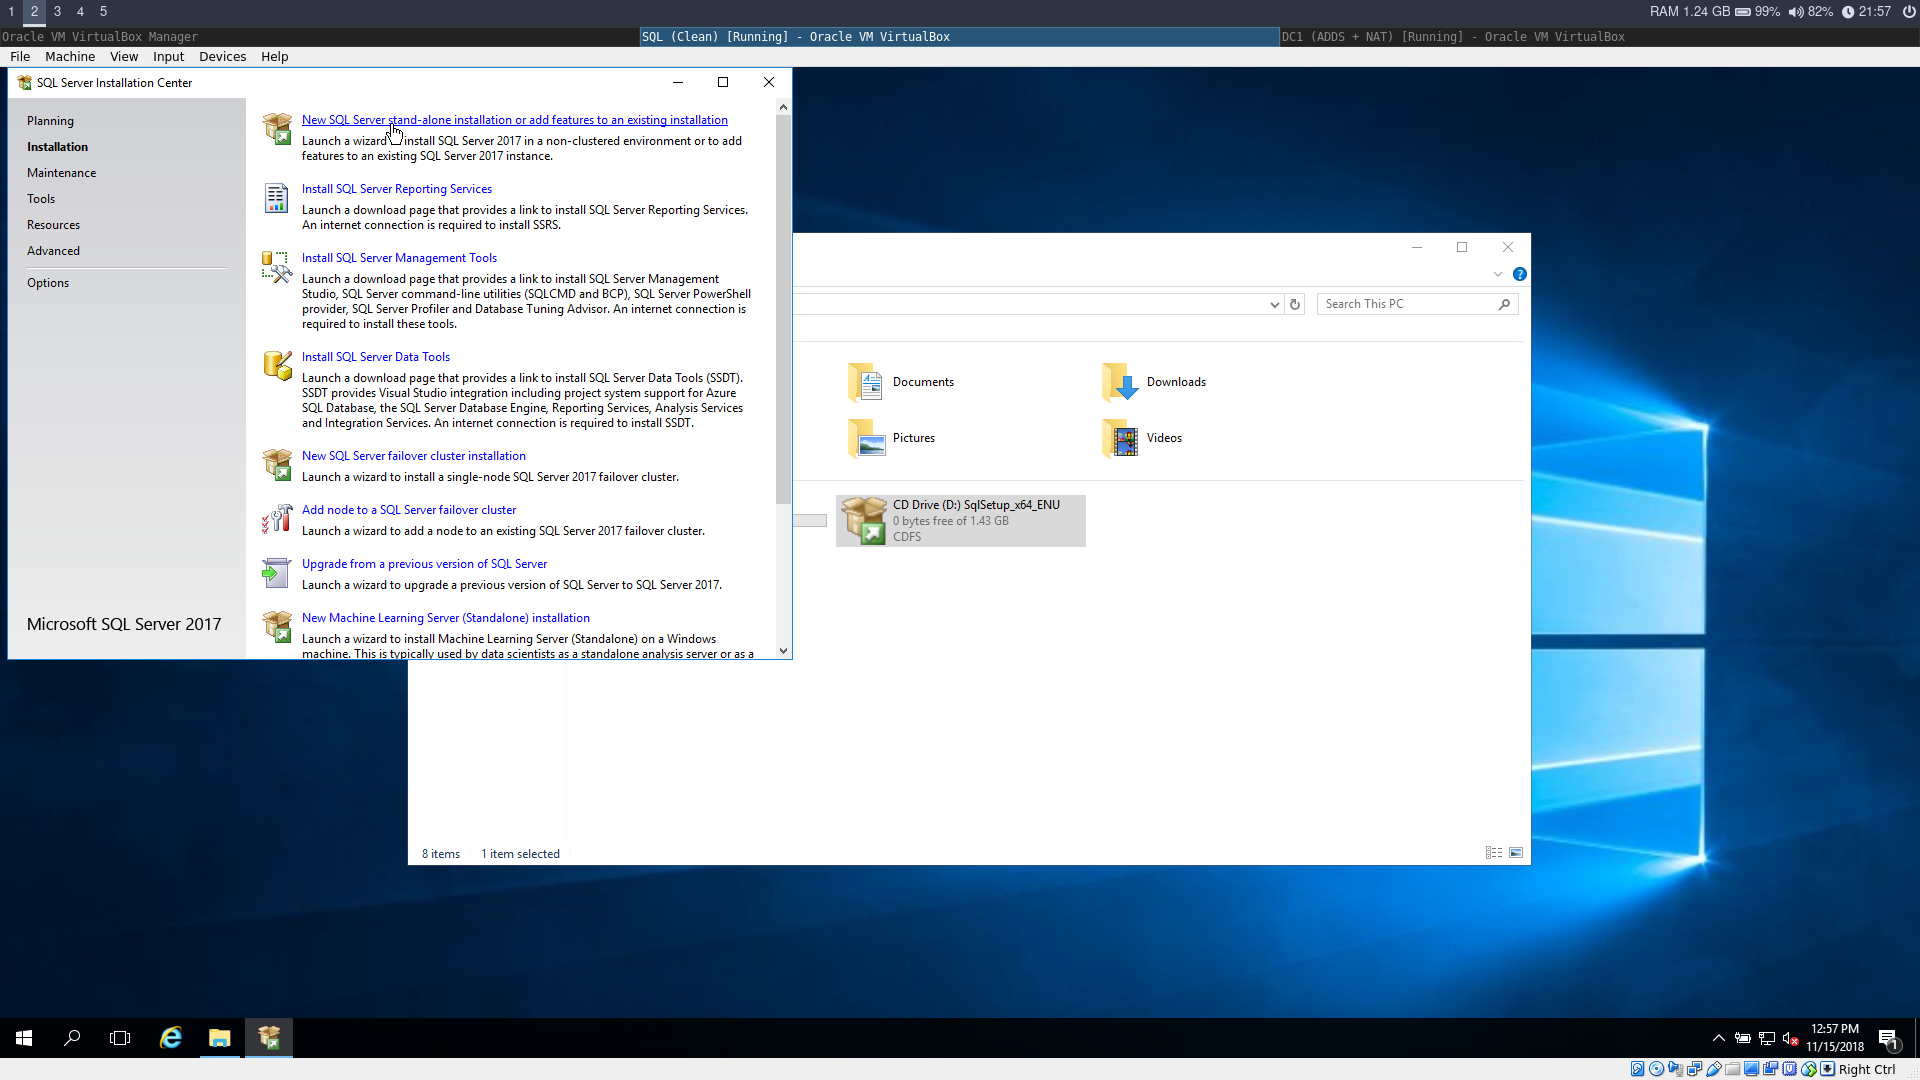
\includegraphics[width=15cm]{Pictures/SQL/1542315469.png}
	
	Start de installatie van de SQL Server.
\end{center}
\begin{center}
	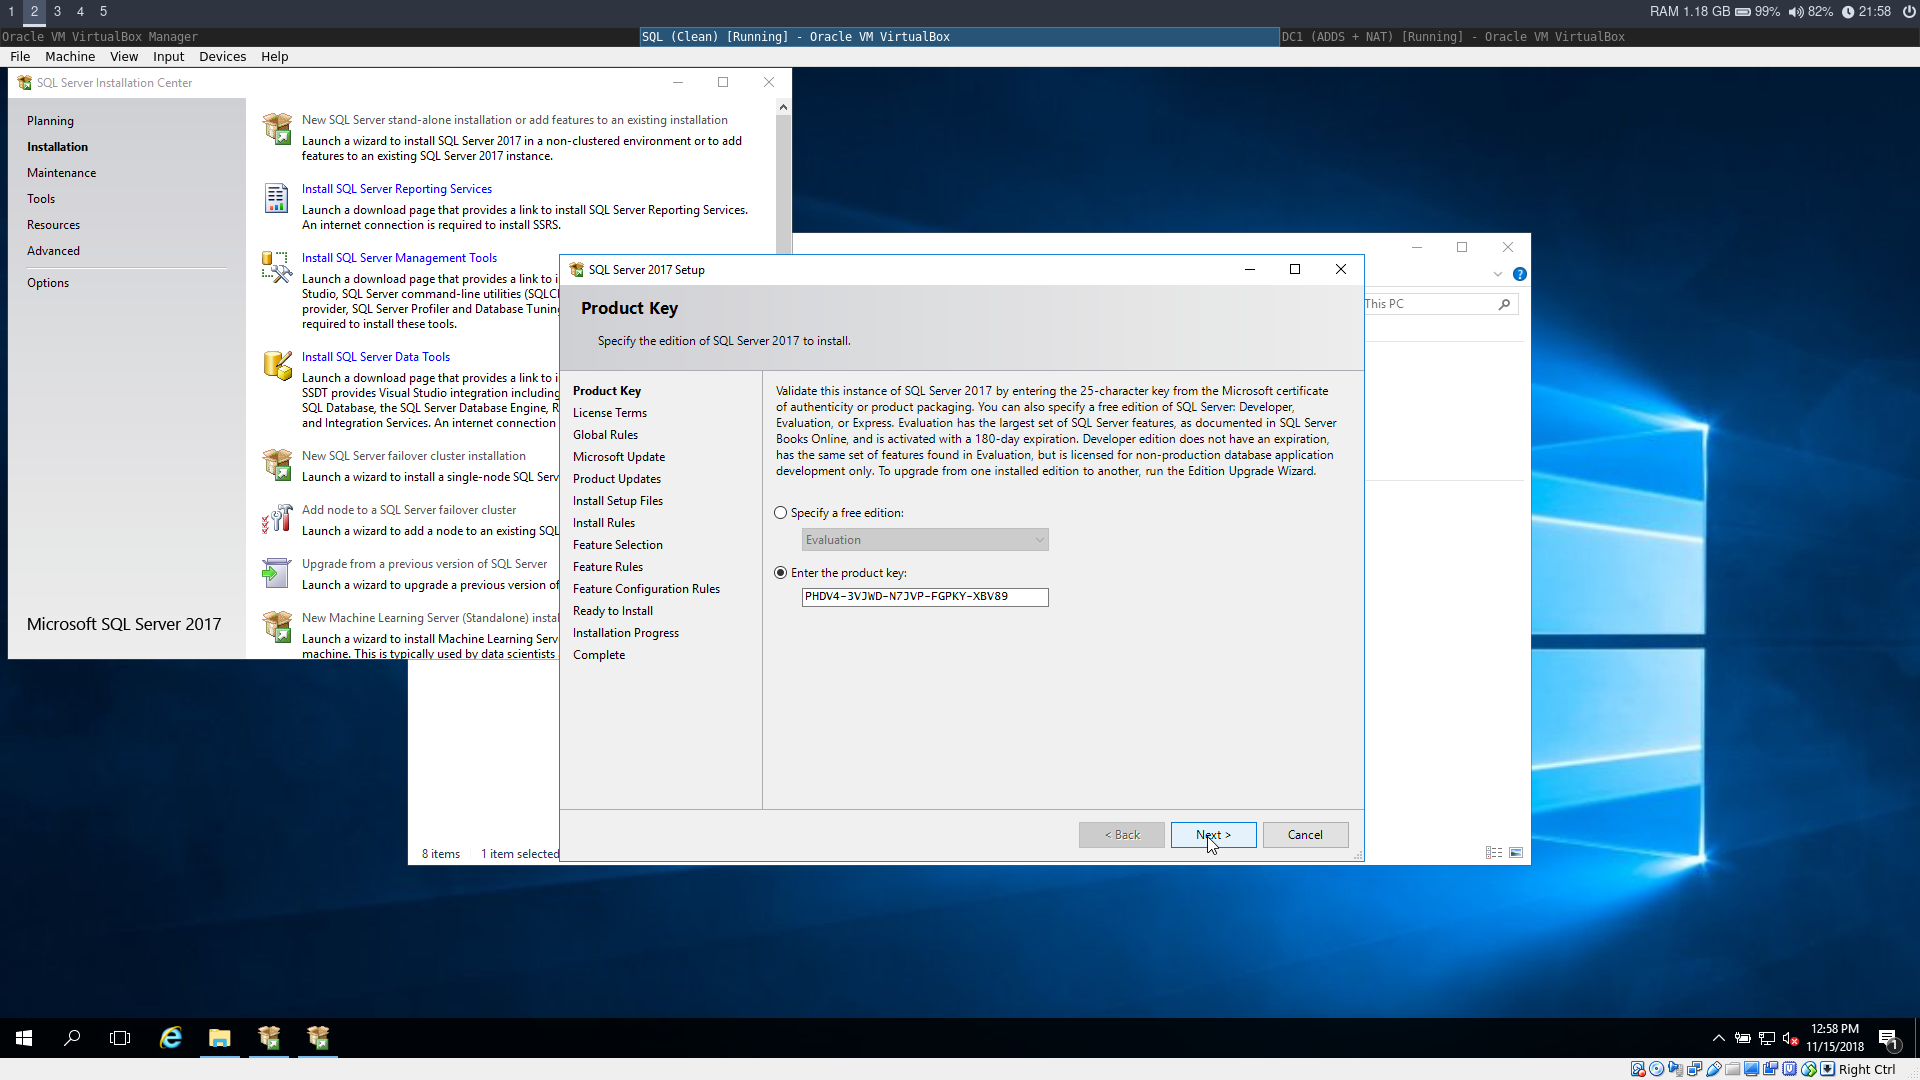
\includegraphics[width=15cm]{Pictures/SQL/1542315497.png}
	
	Voer de licentiecode in.
\end{center}
\begin{center}
	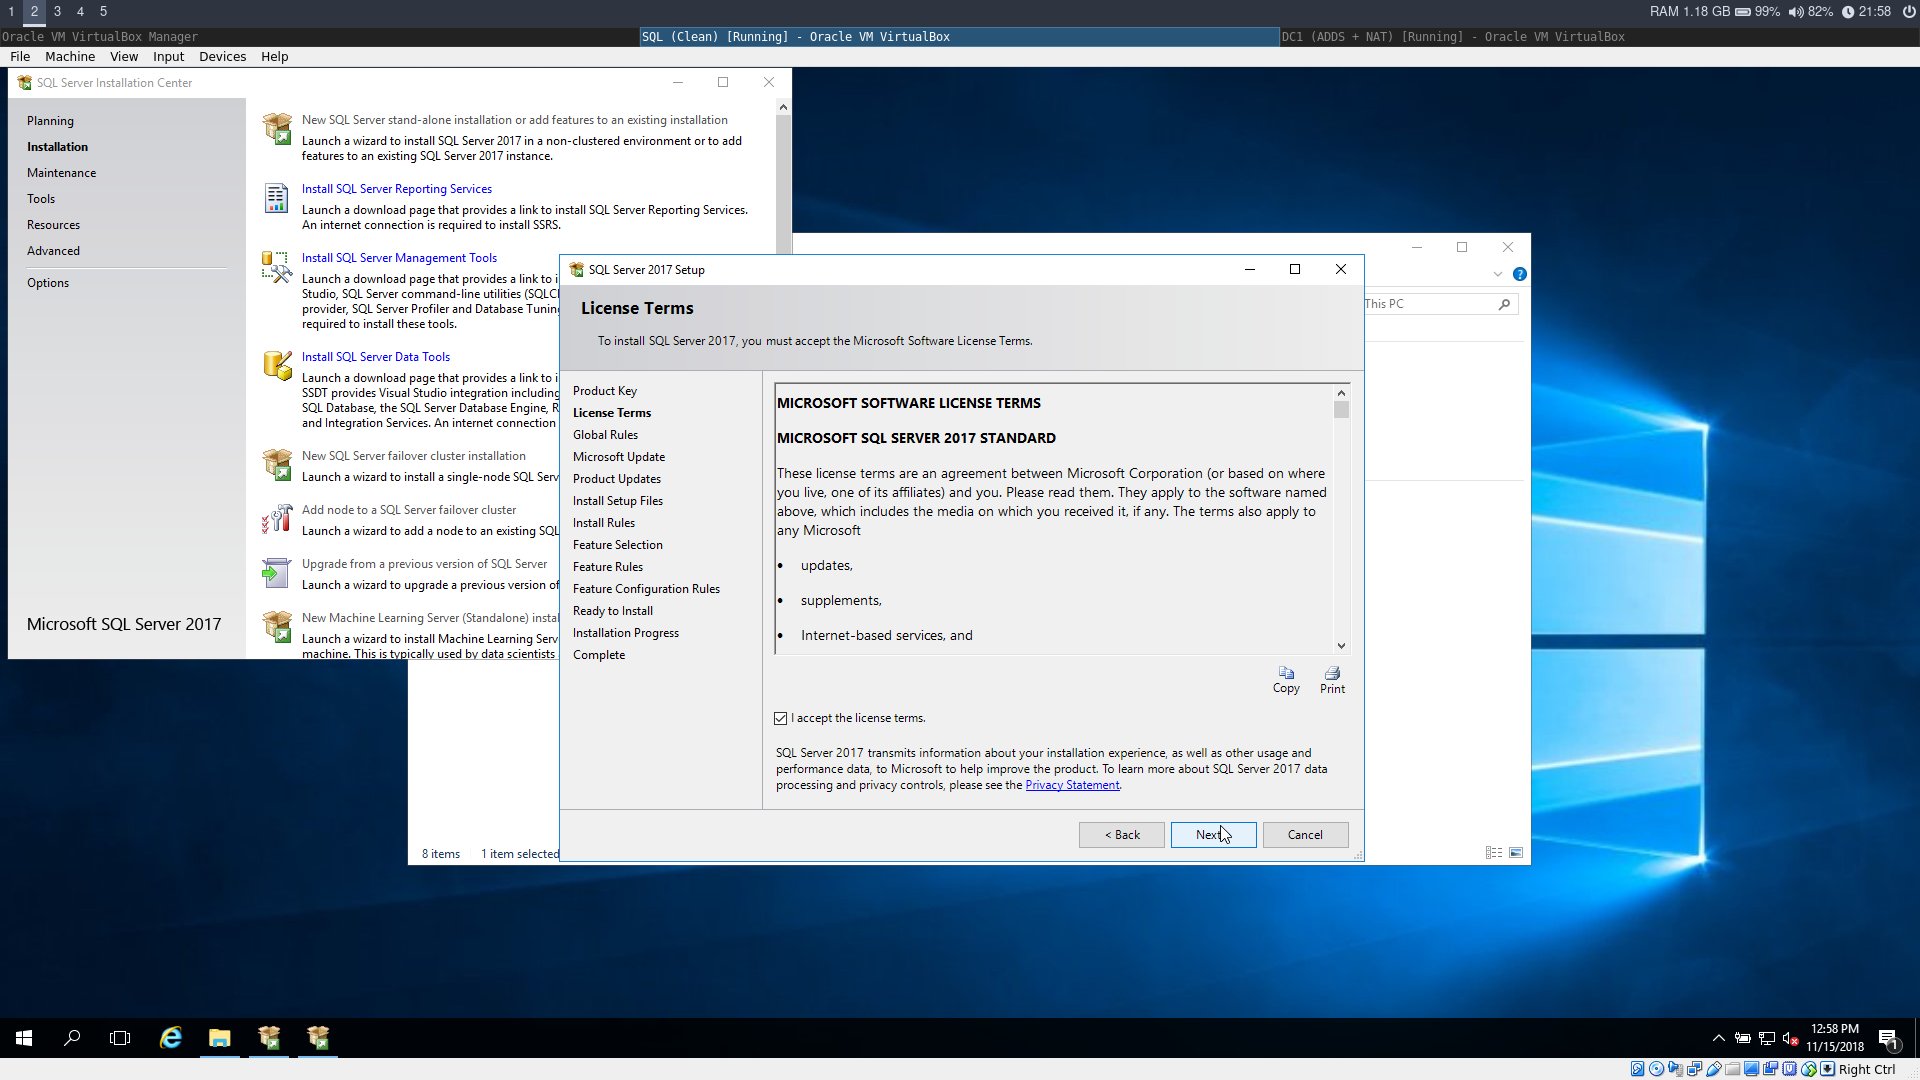
\includegraphics[width=15cm]{Pictures/SQL/1542315502.png}
	
	Volg de installatiewizard.
\end{center}
\begin{center}
	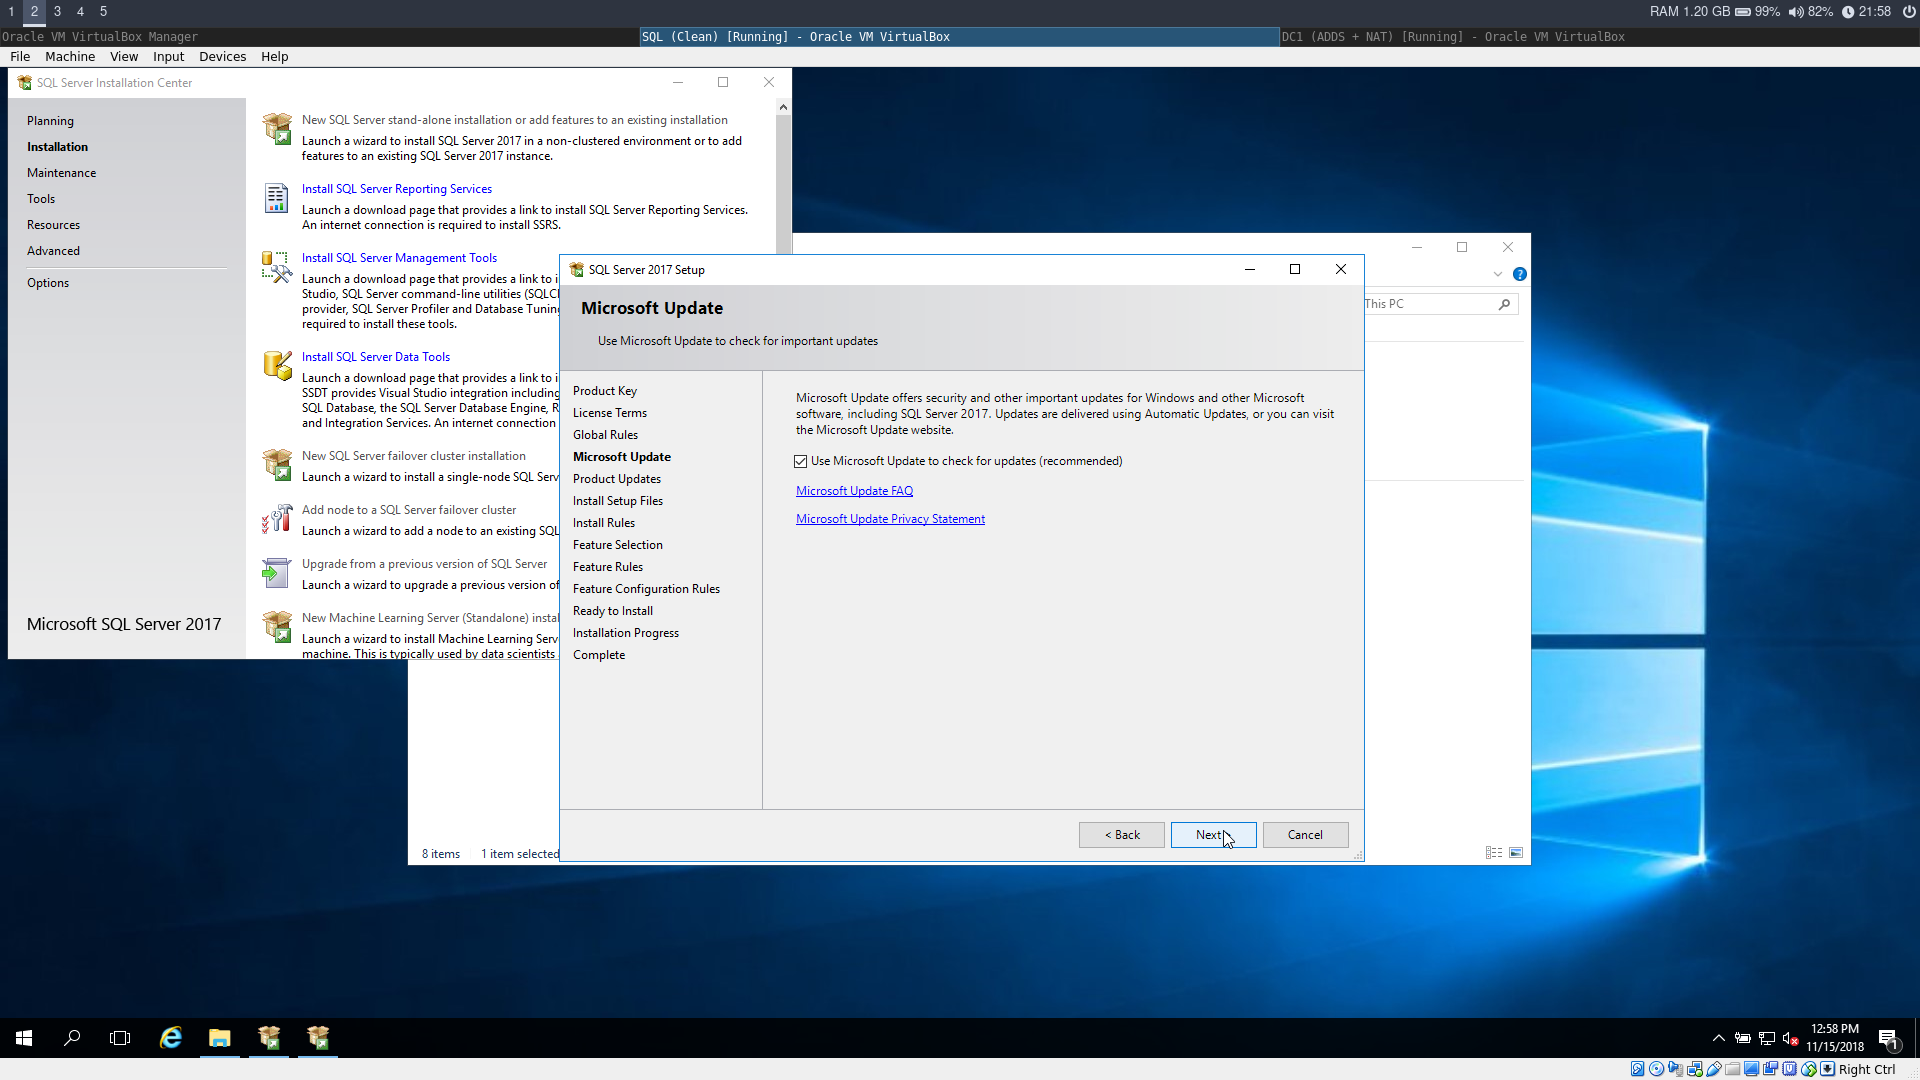
\includegraphics[width=15cm]{Pictures/SQL/1542315511.png}
	
	Accepteer de licentievoorwaarden.
\end{center}
\begin{center}
	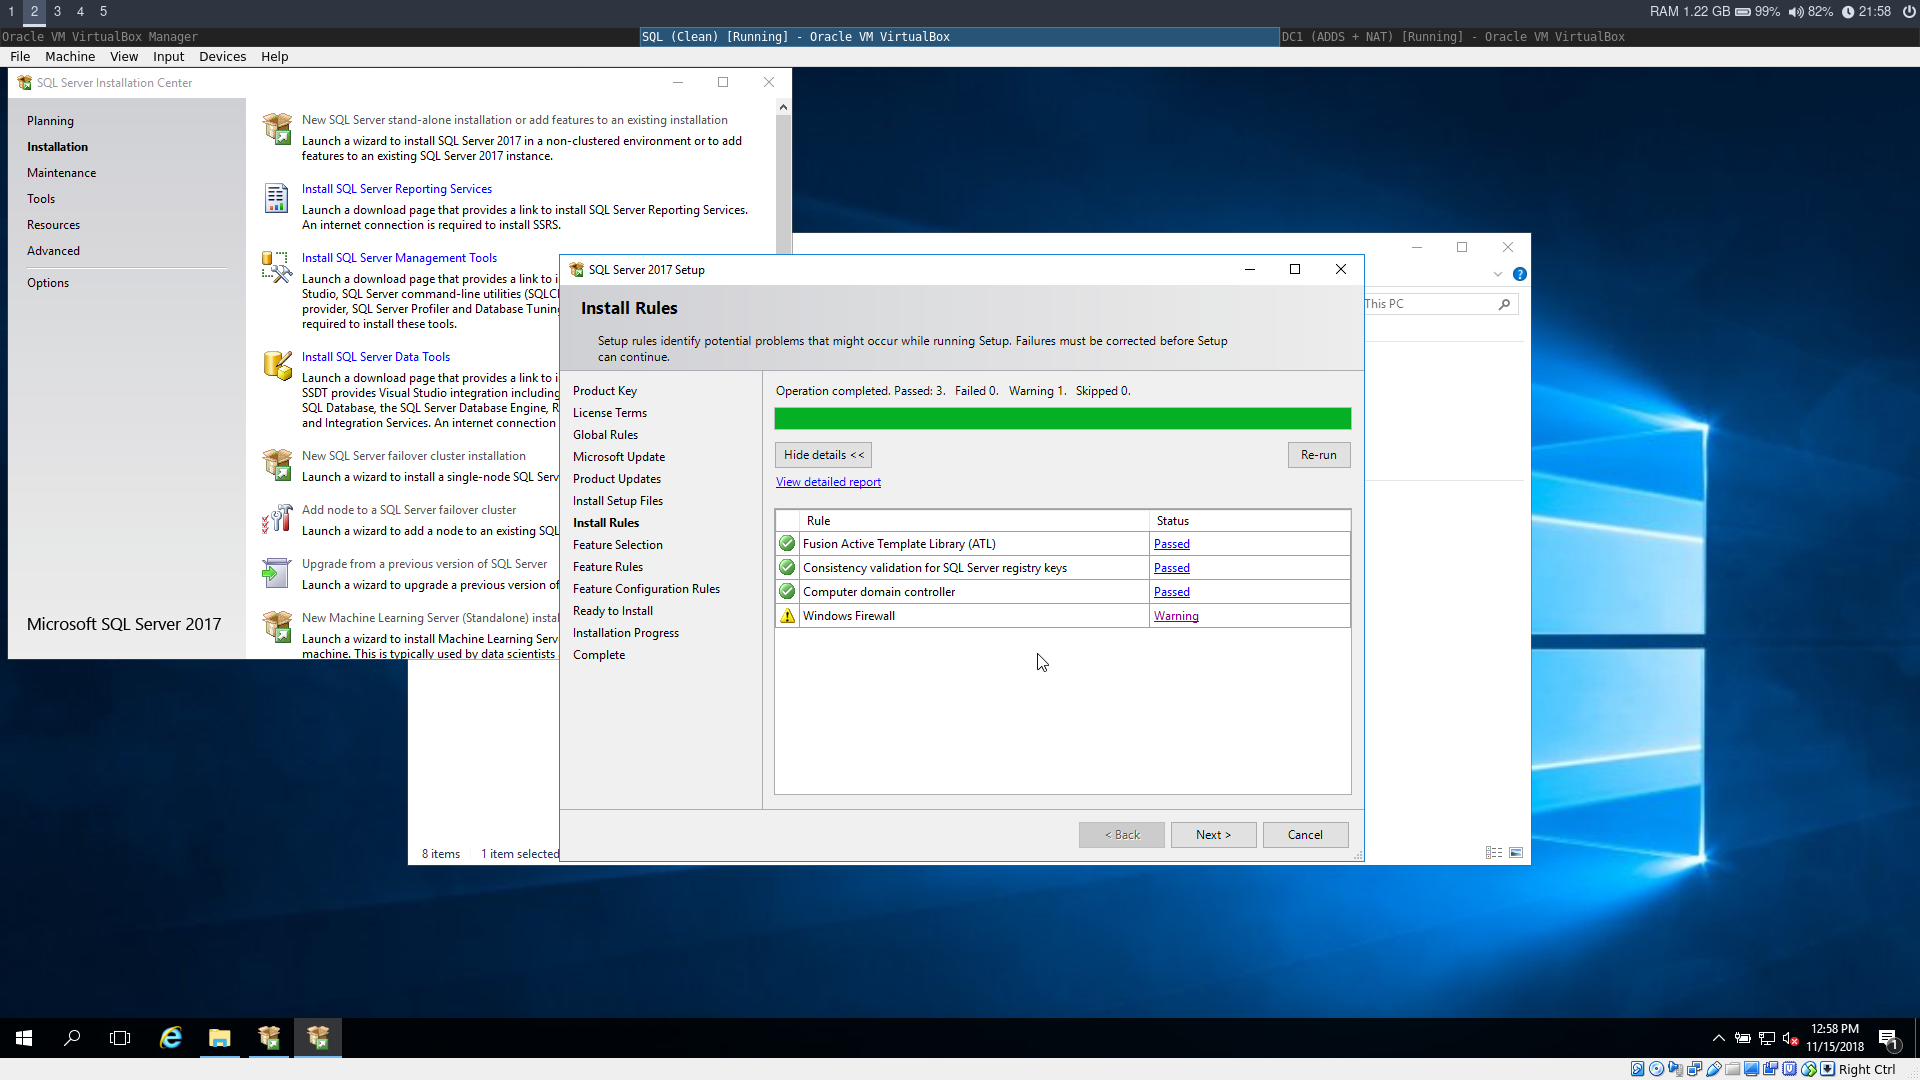
\includegraphics[width=15cm]{Pictures/SQL/1542315538.png}
	
	Indien een waarschuwing bij de Firewall gegeven wordt, moet een regel toegevoegd worden.
\end{center}
\begin{center}
	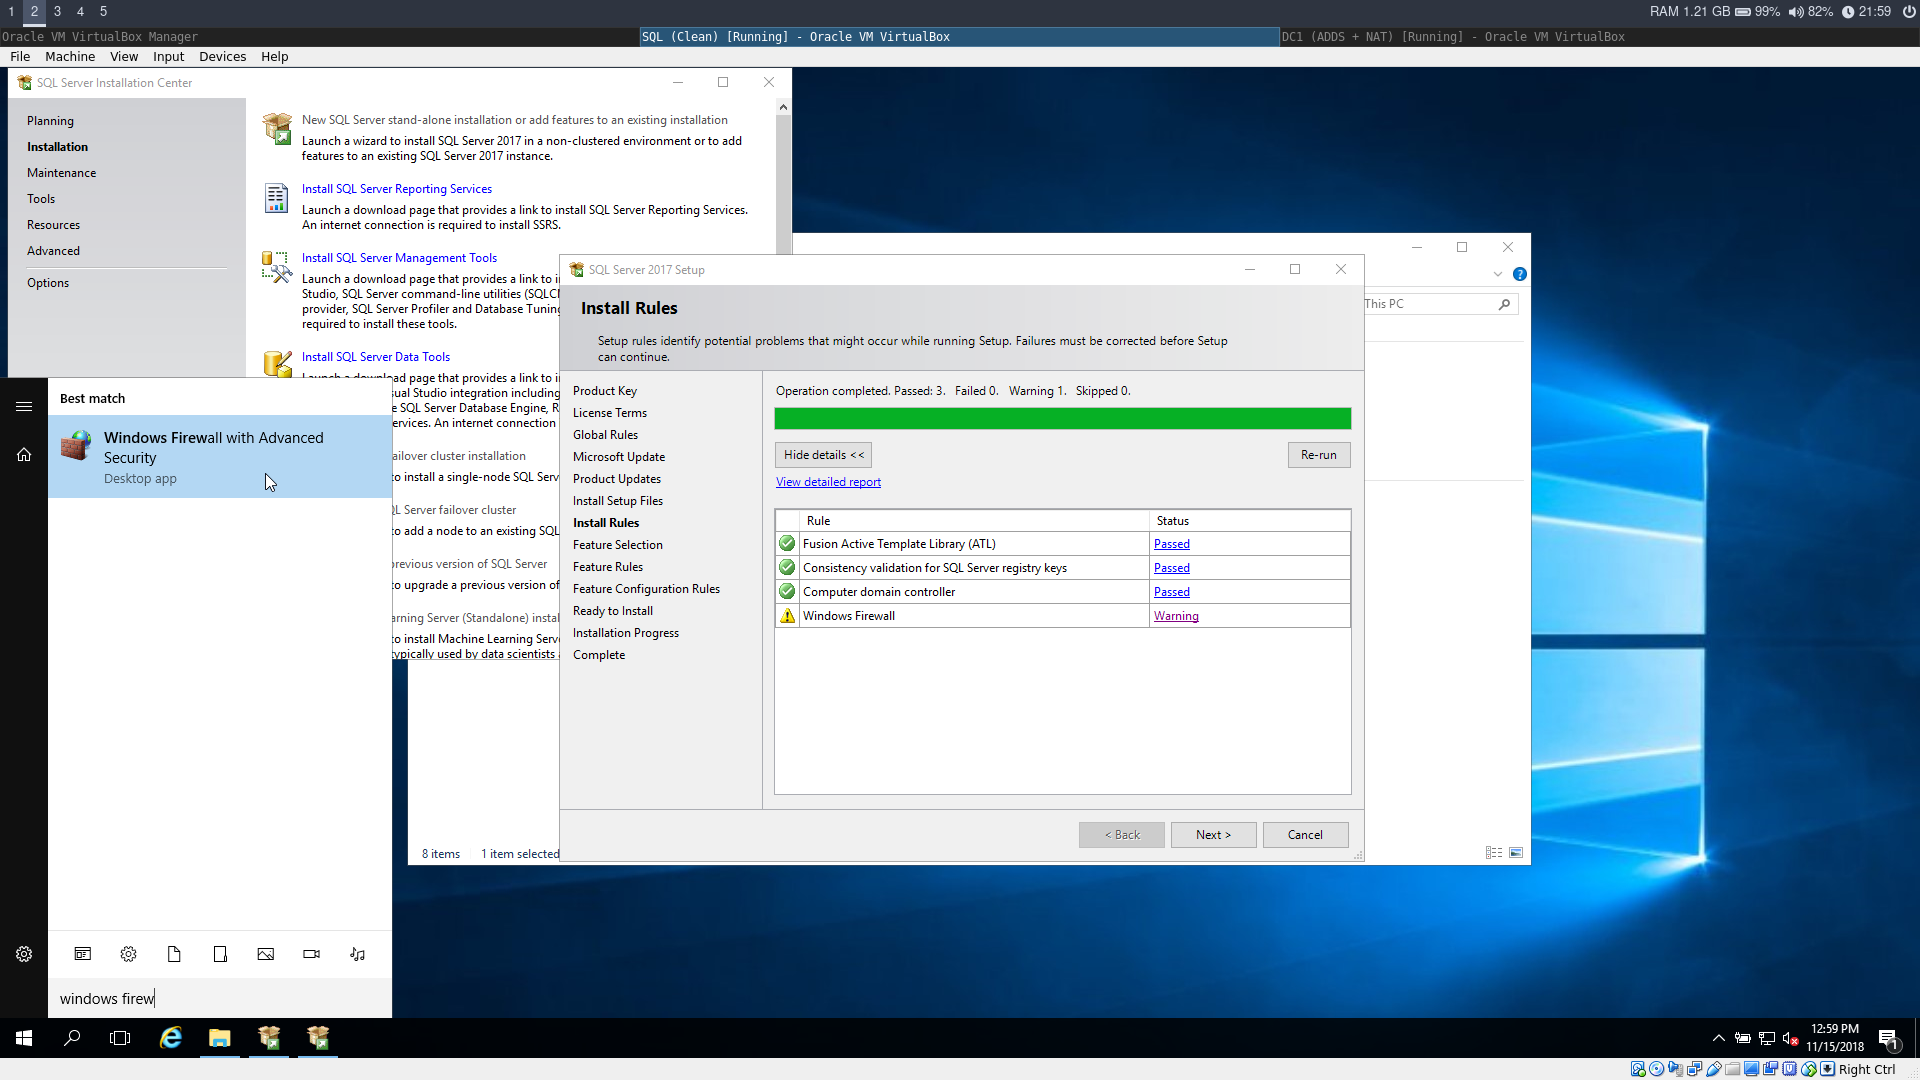
\includegraphics[width=15cm]{Pictures/SQL/1542315570.png}
\end{center}
\begin{center}
	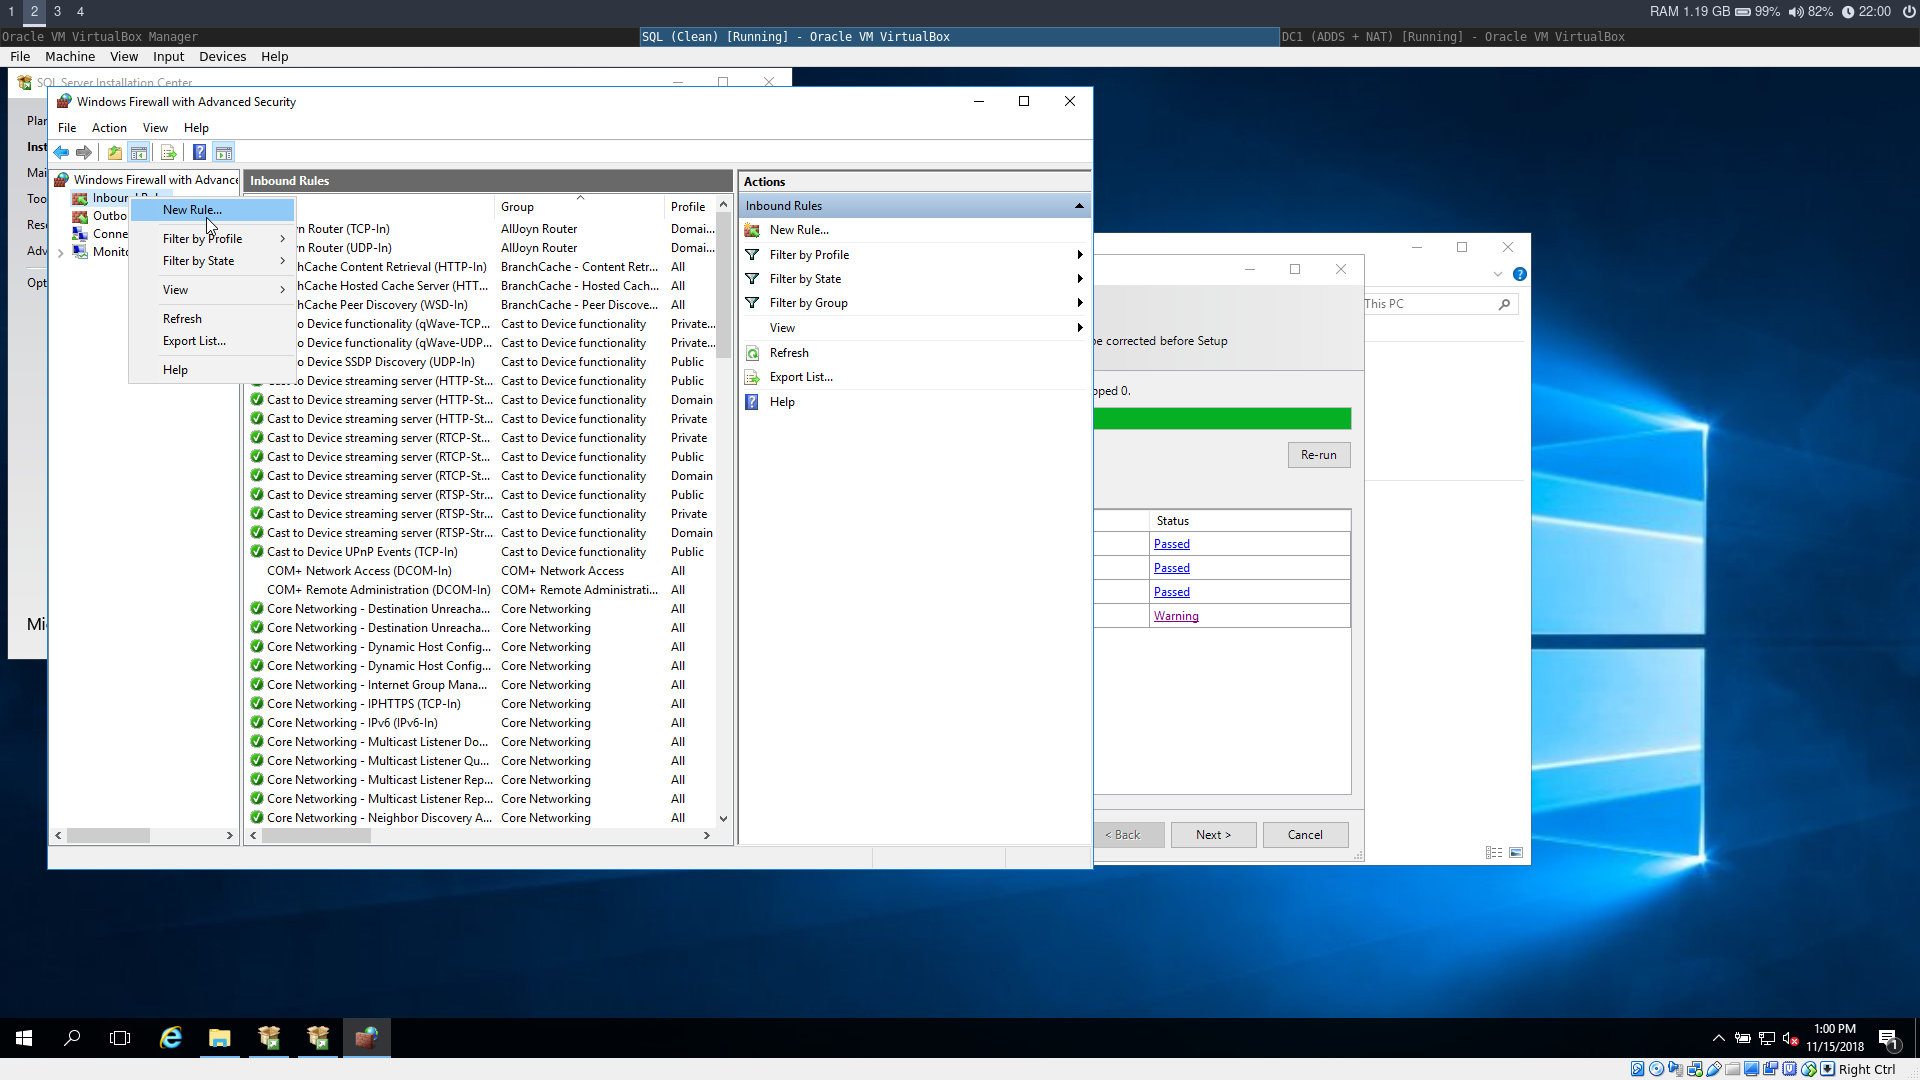
\includegraphics[width=15cm]{Pictures/SQL/1542315603.png}
\end{center}
\begin{center}
	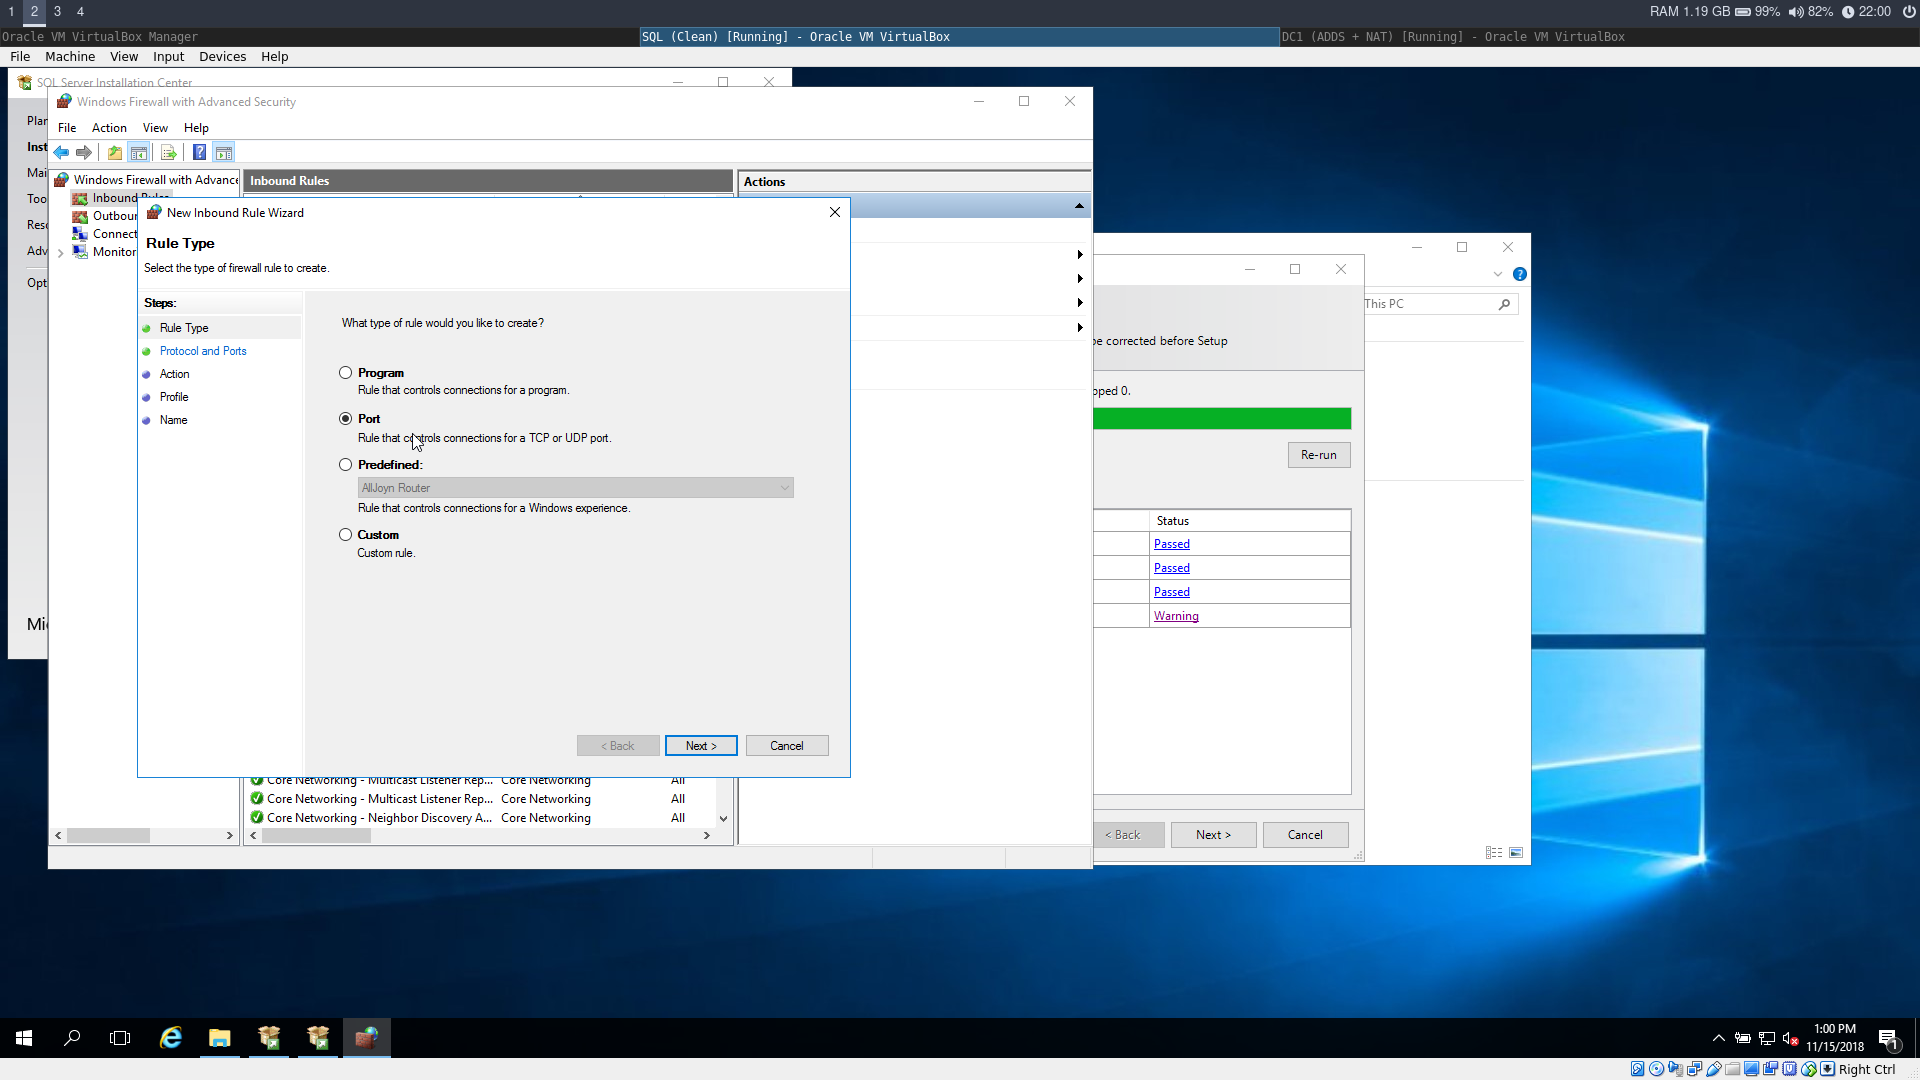
\includegraphics[width=15cm]{Pictures/SQL/1542315607.png}
	
	Volg de configuratiewizard.
\end{center}
\begin{center}
	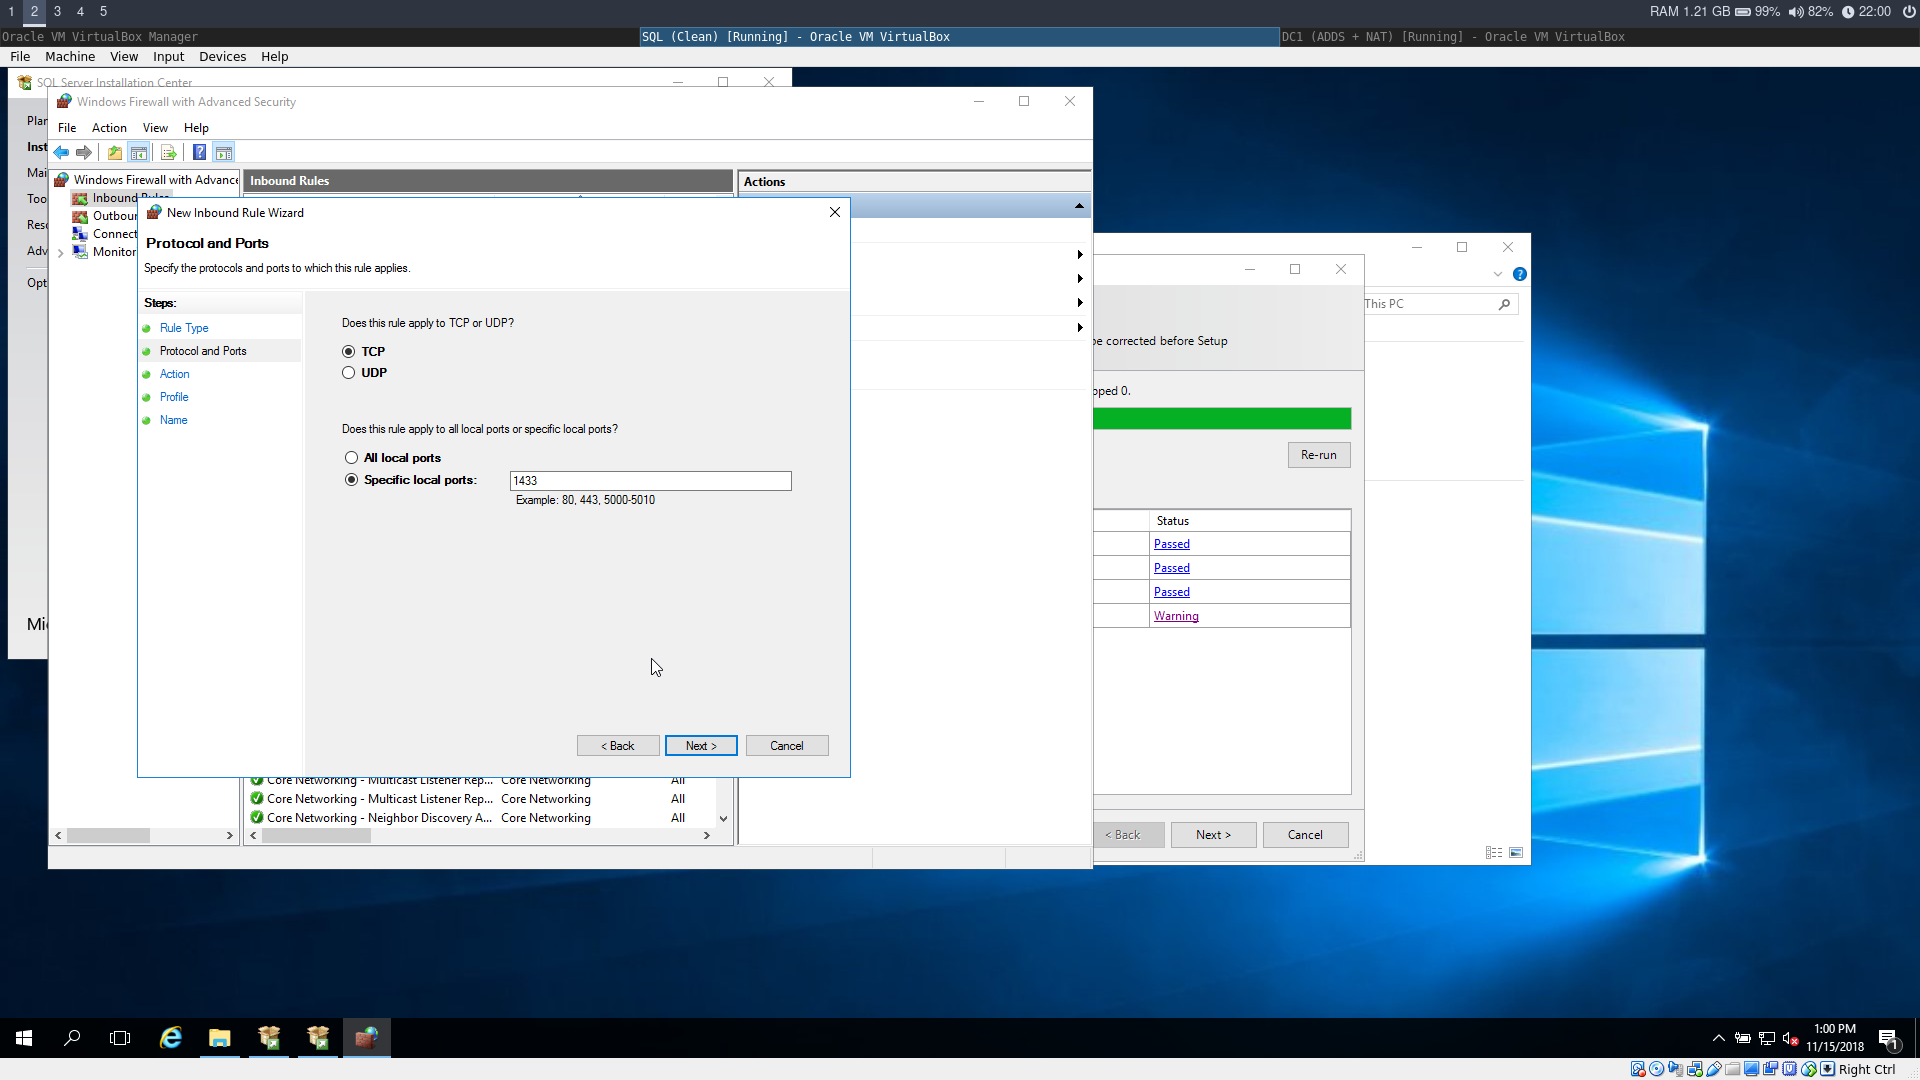
\includegraphics[width=15cm]{Pictures/SQL/1542315658.png}
\end{center}
\begin{center}
	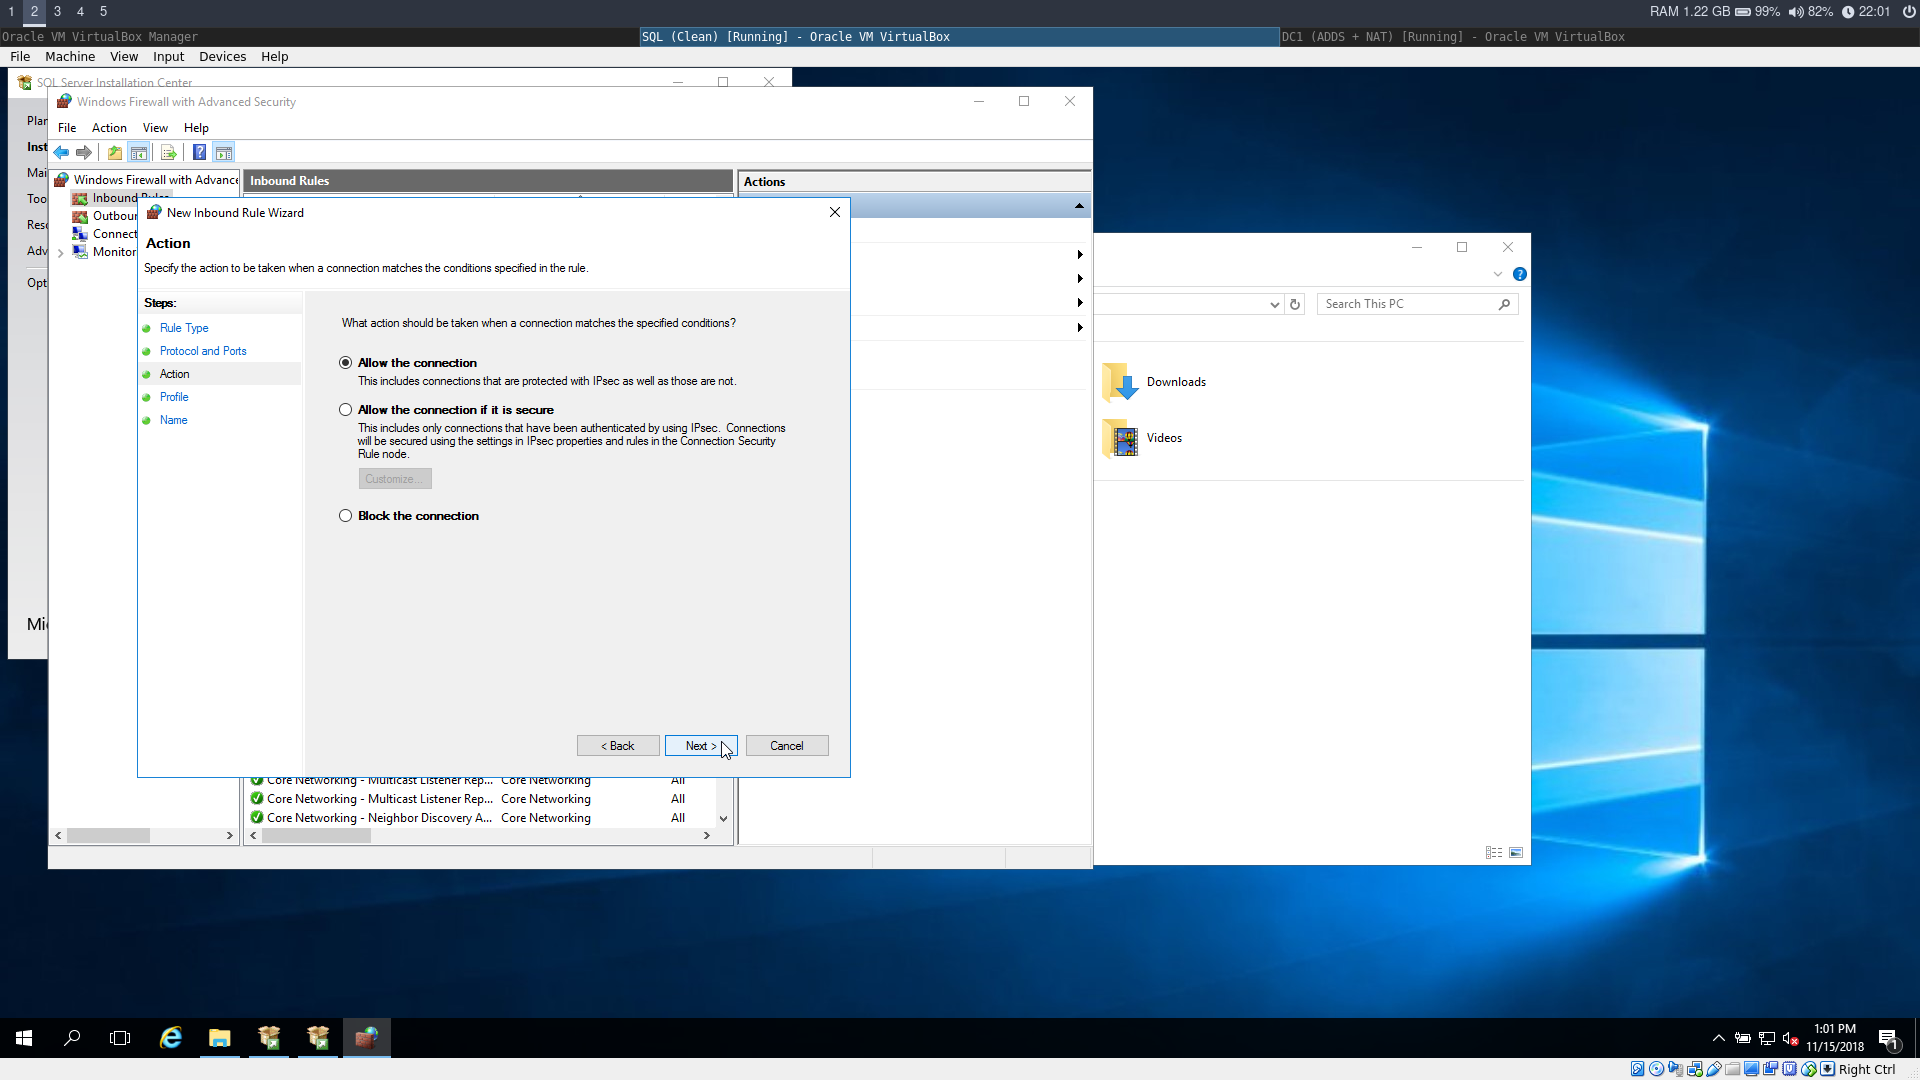
\includegraphics[width=15cm]{Pictures/SQL/1542315671.png}
\end{center}
\begin{center}
	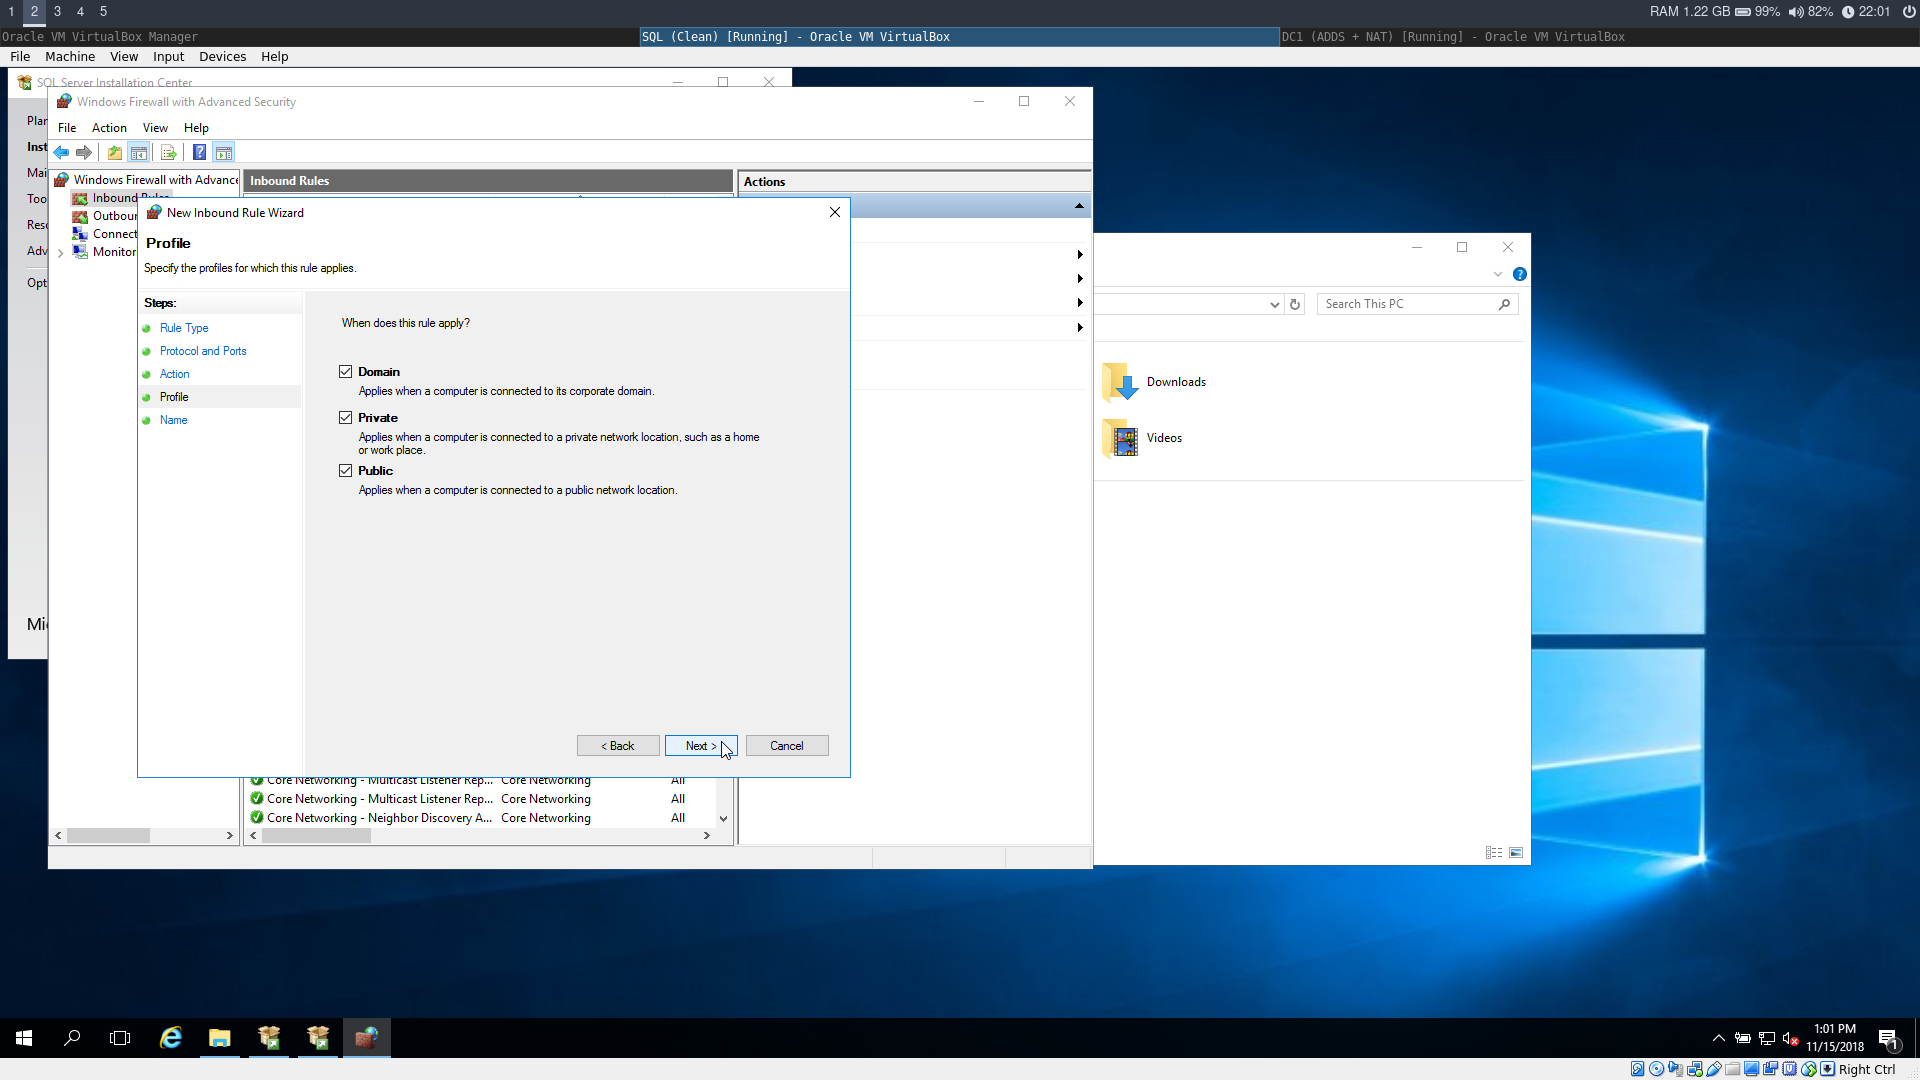
\includegraphics[width=15cm]{Pictures/SQL/1542315673.png}
\end{center}
\begin{center}
	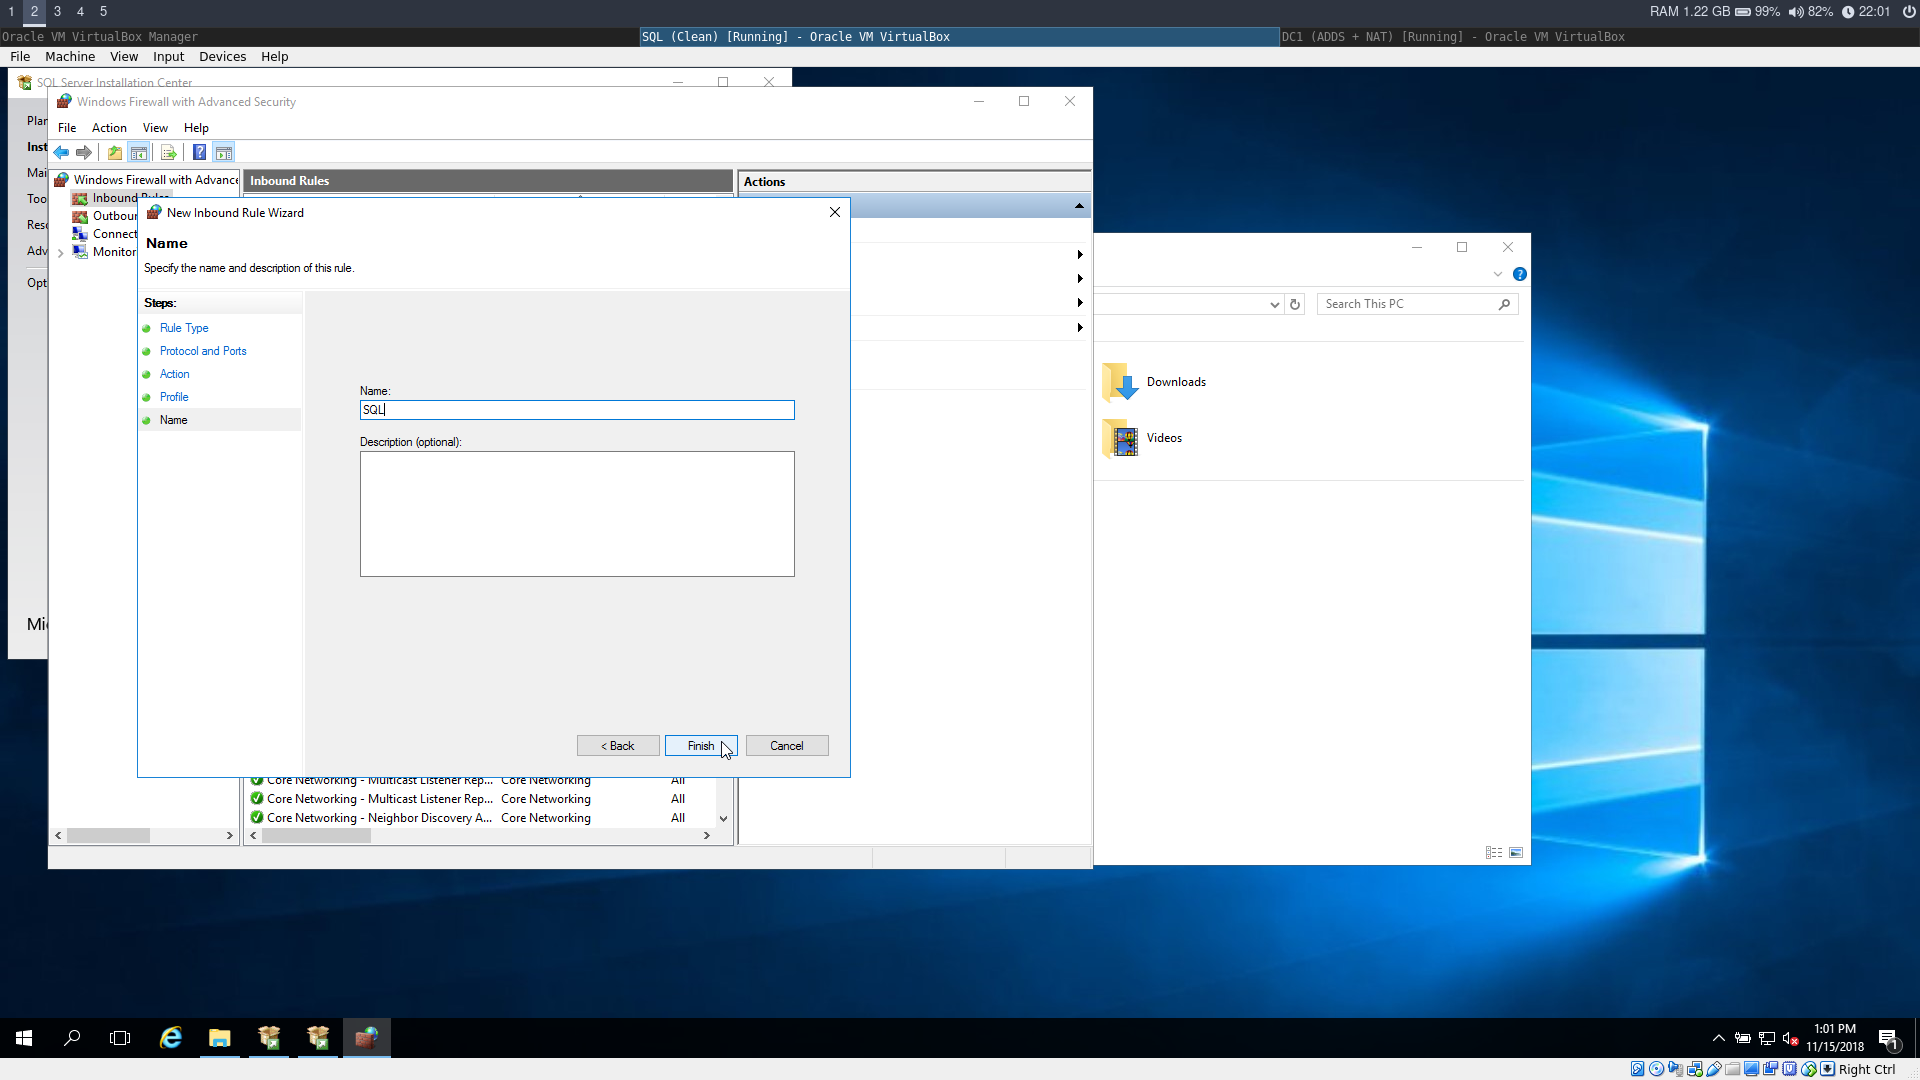
\includegraphics[width=15cm]{Pictures/SQL/1542315679.png}
\end{center}
\begin{center}
	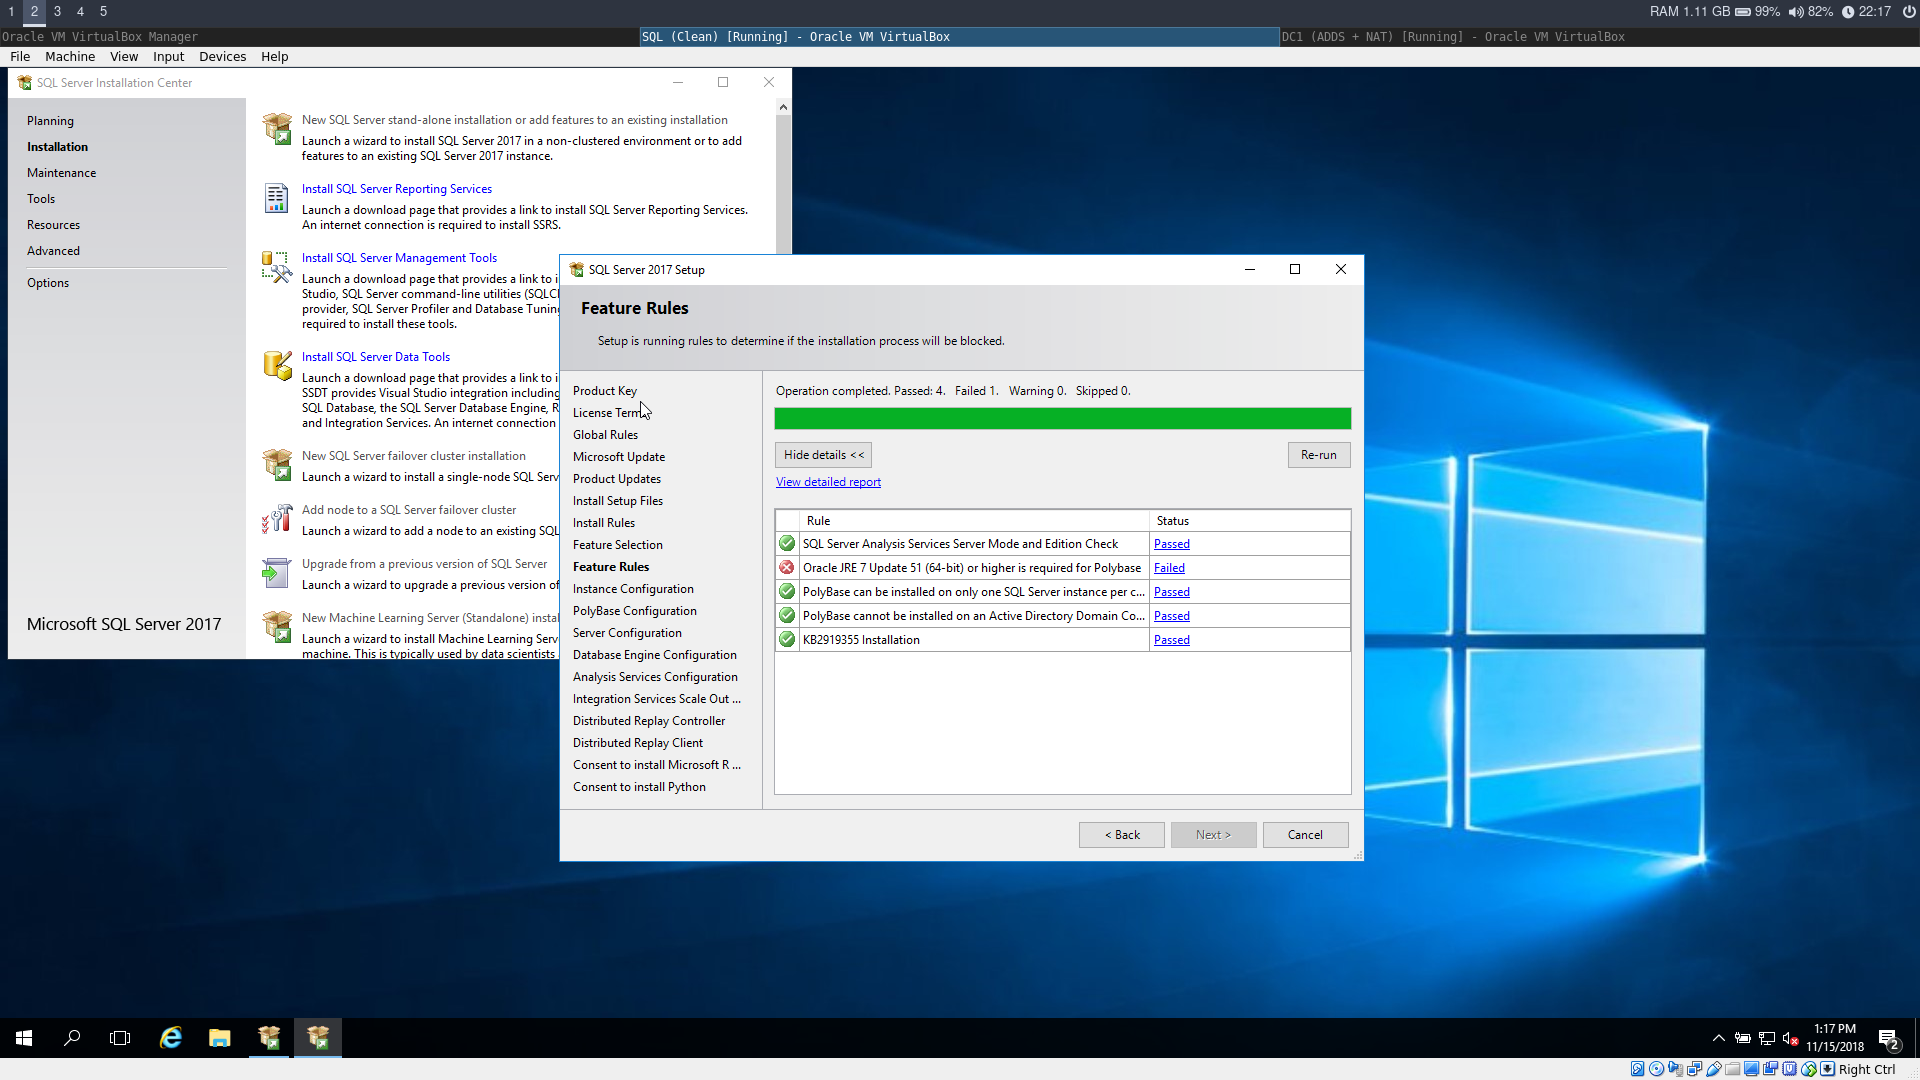
\includegraphics[width=15cm]{Pictures/SQL/1542316632.png}
	
	Bij deze foutmelding dient Oracle JRE (Java) geïnstalleerd te worden.
\end{center}
\begin{center}
	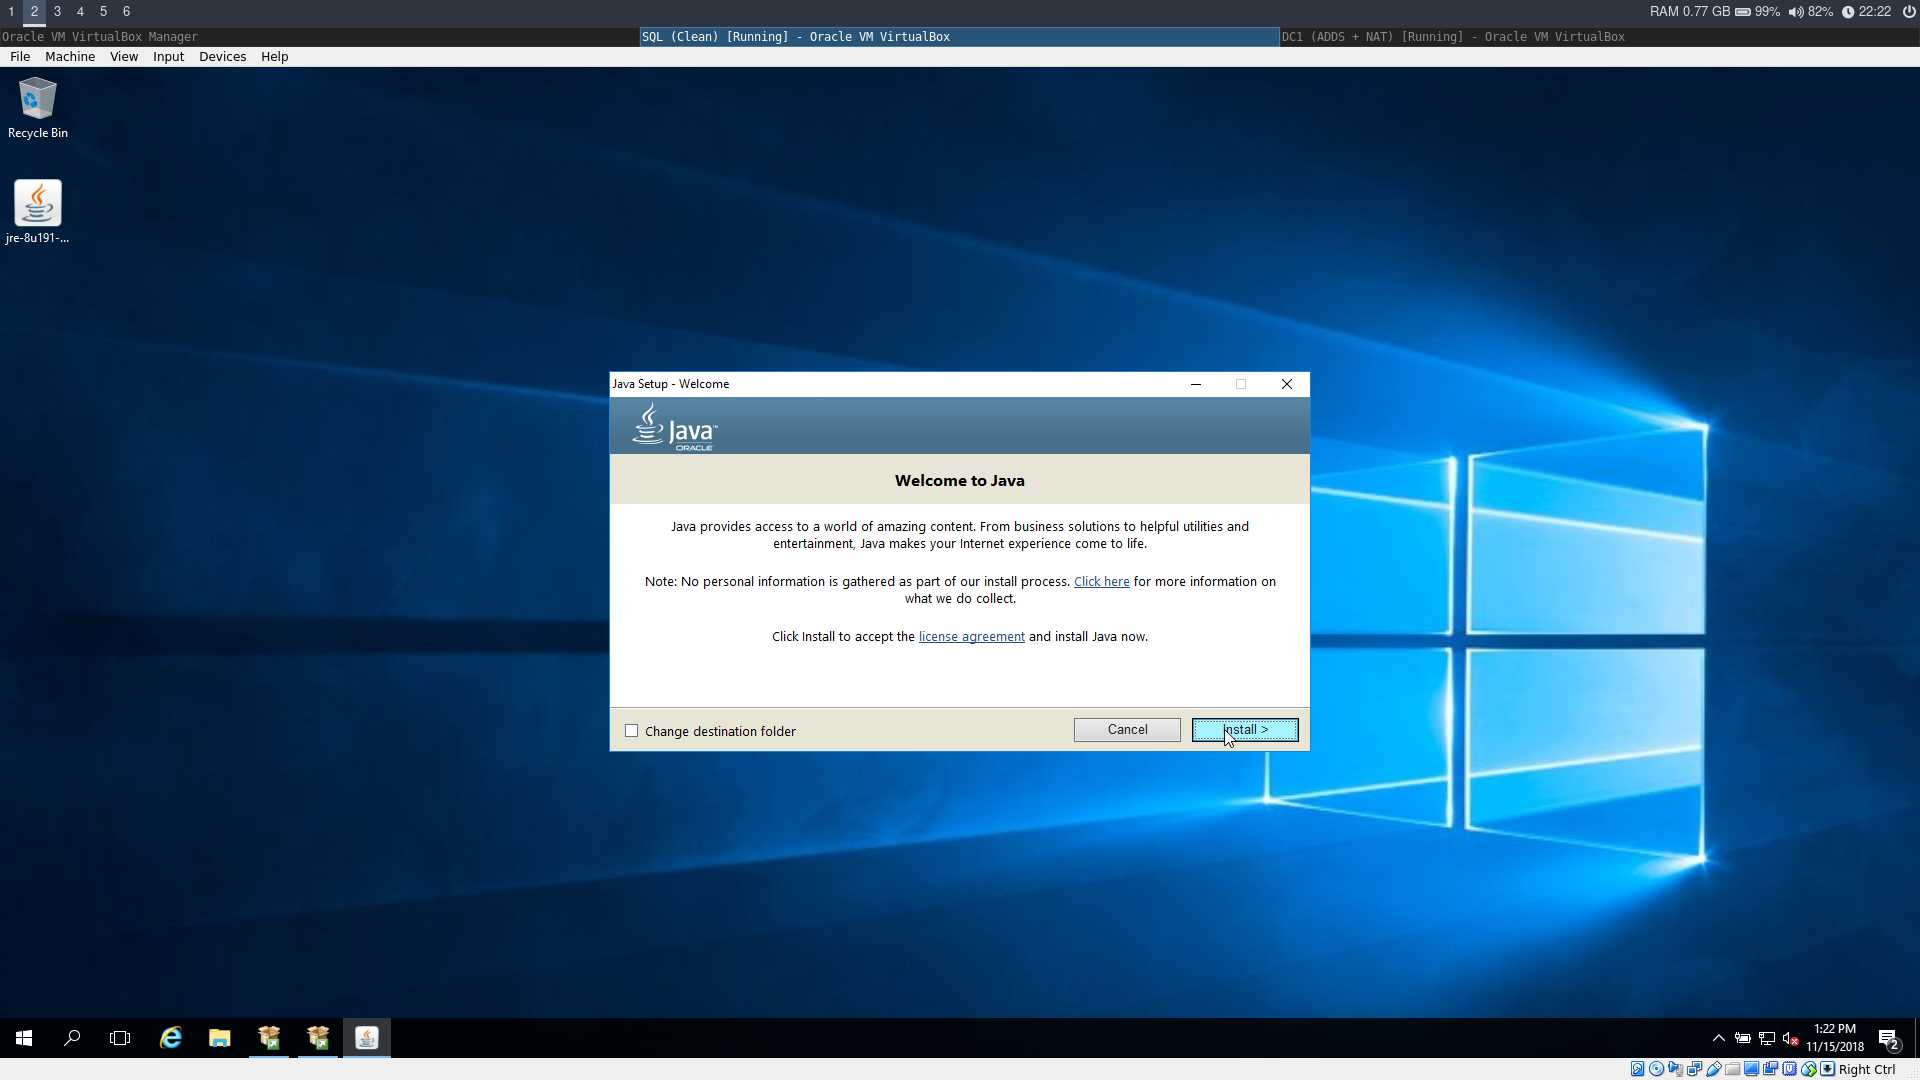
\includegraphics[width=15cm]{Pictures/SQL/1542316945.png}
	
	Volg de installatiewizard.
\end{center}
\begin{center}
	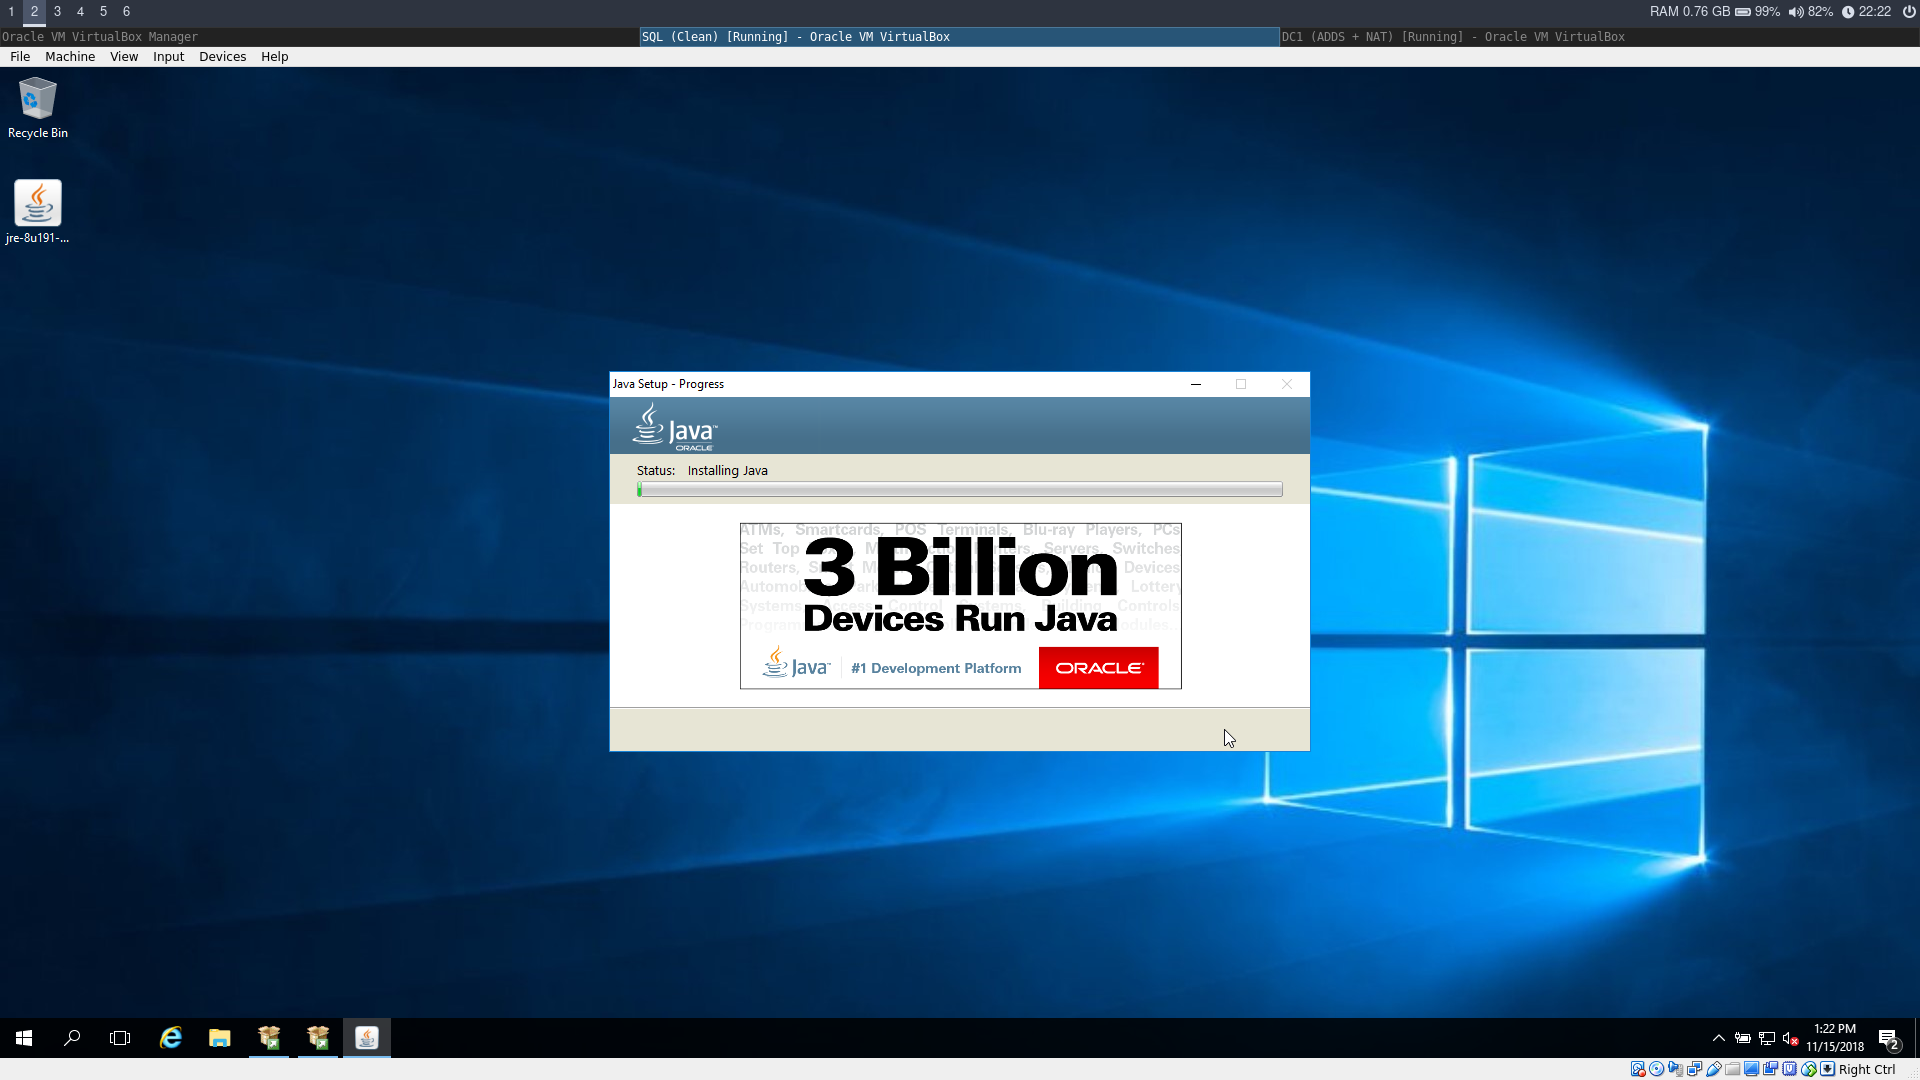
\includegraphics[width=15cm]{Pictures/SQL/1542316953.png}
\end{center}
\begin{center}
	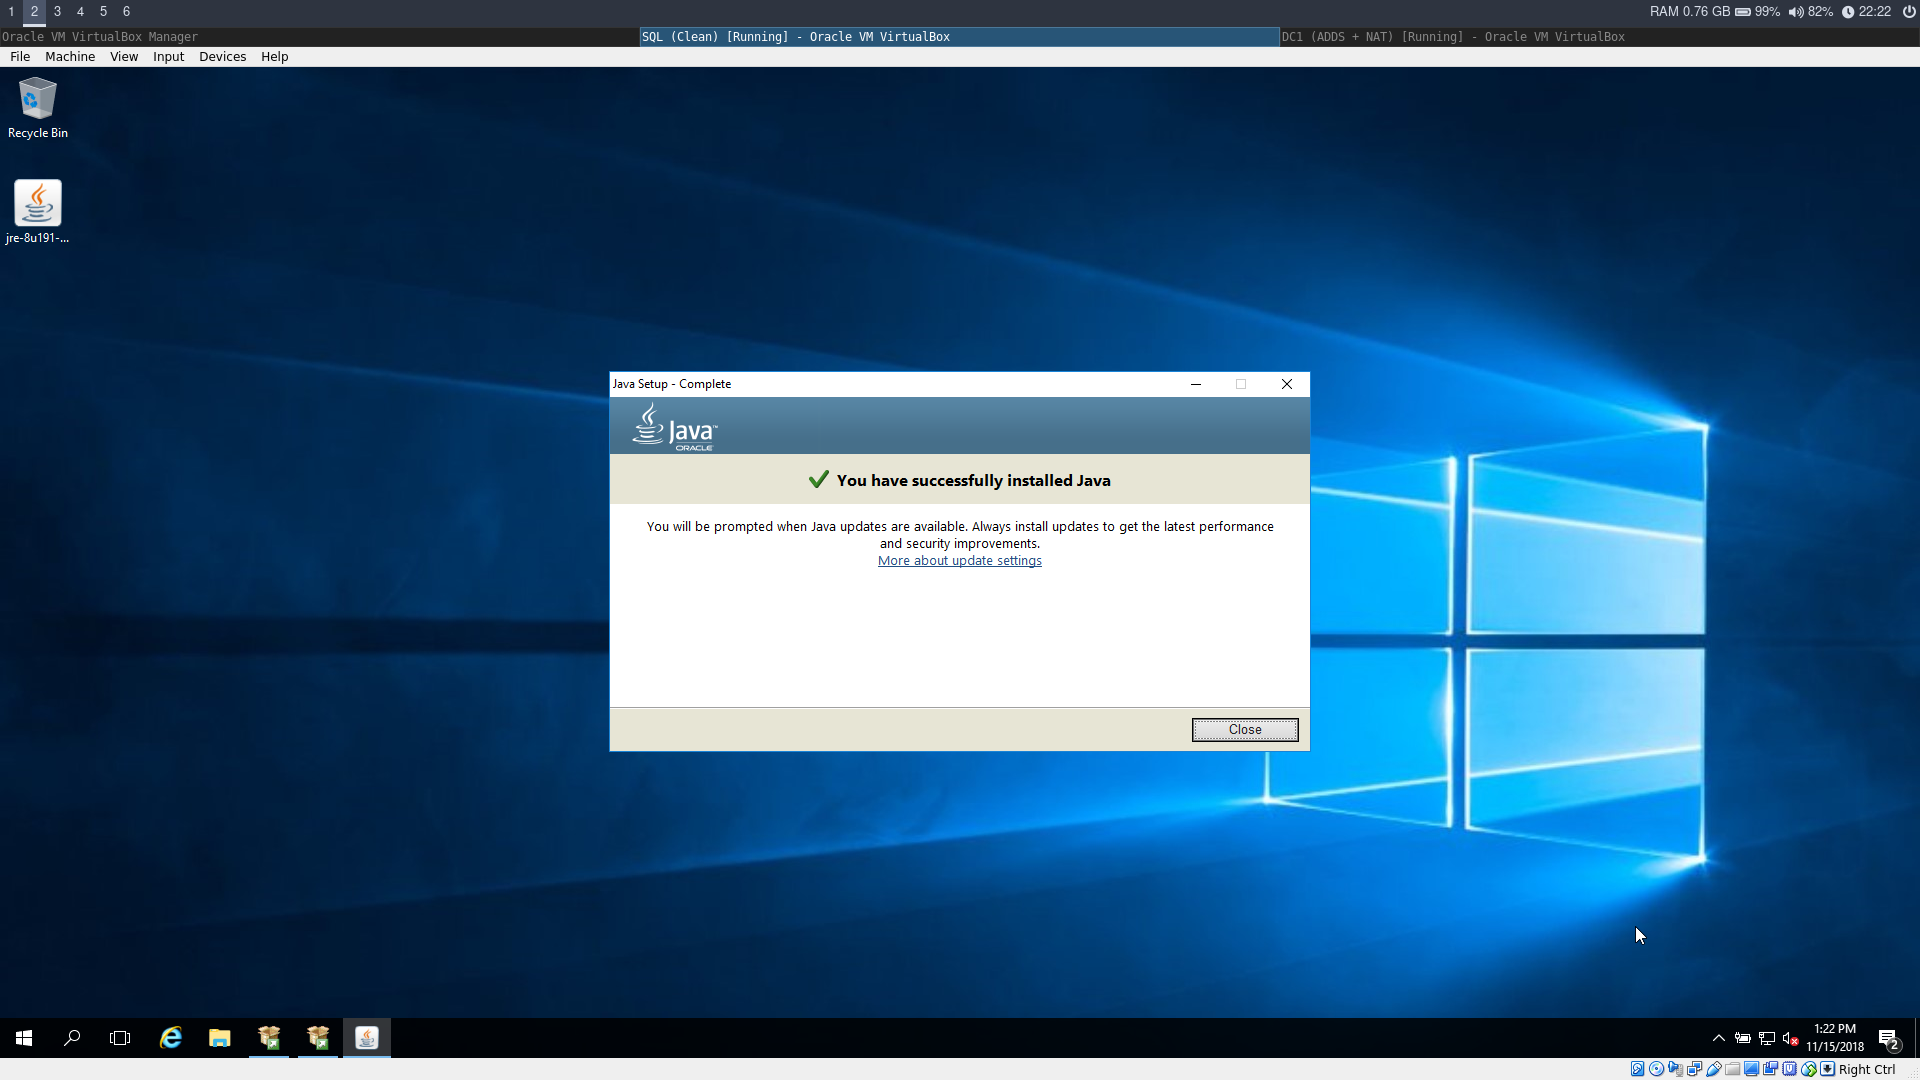
\includegraphics[width=15cm]{Pictures/SQL/1542316980.png}
\end{center}
\begin{center}
	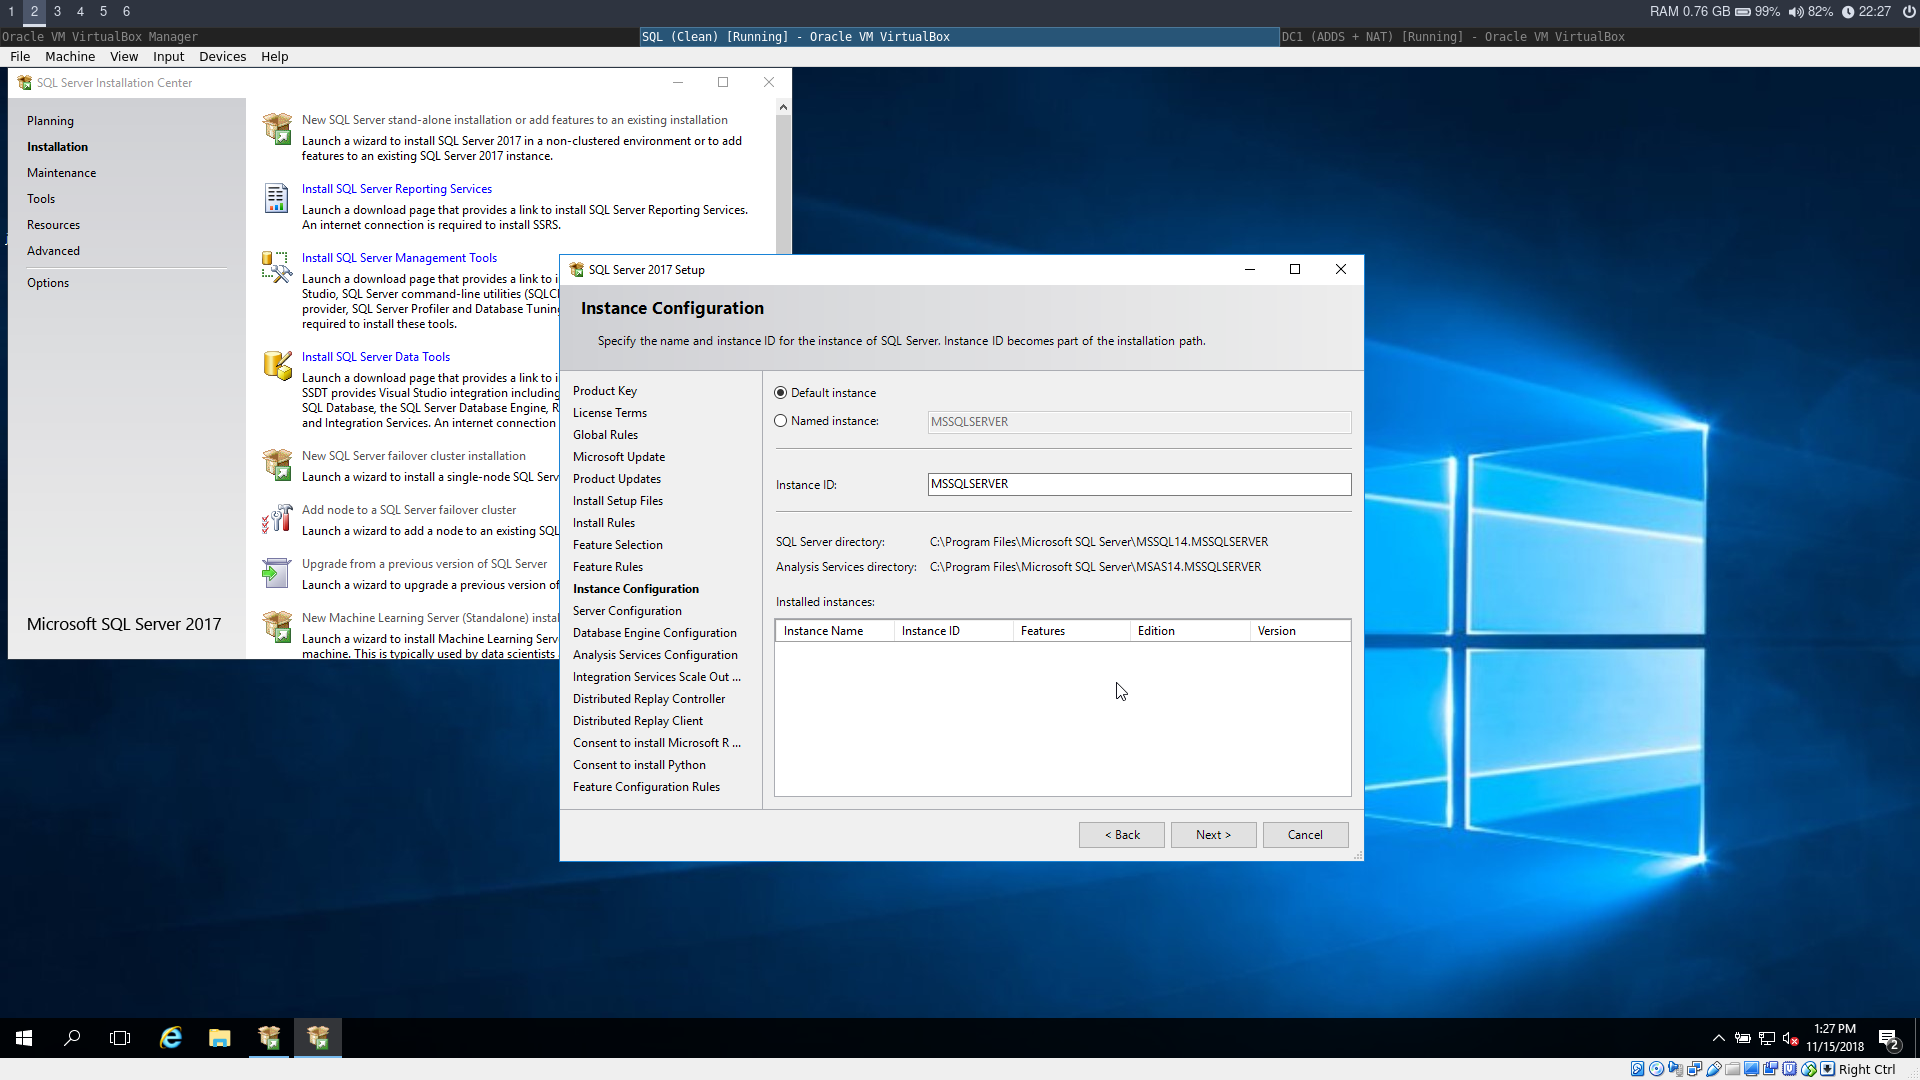
\includegraphics[width=15cm]{Pictures/SQL/1542317256.png}
	
	Ga verder met de installatiewizard voor SQL Server.
\end{center}
\begin{center}
	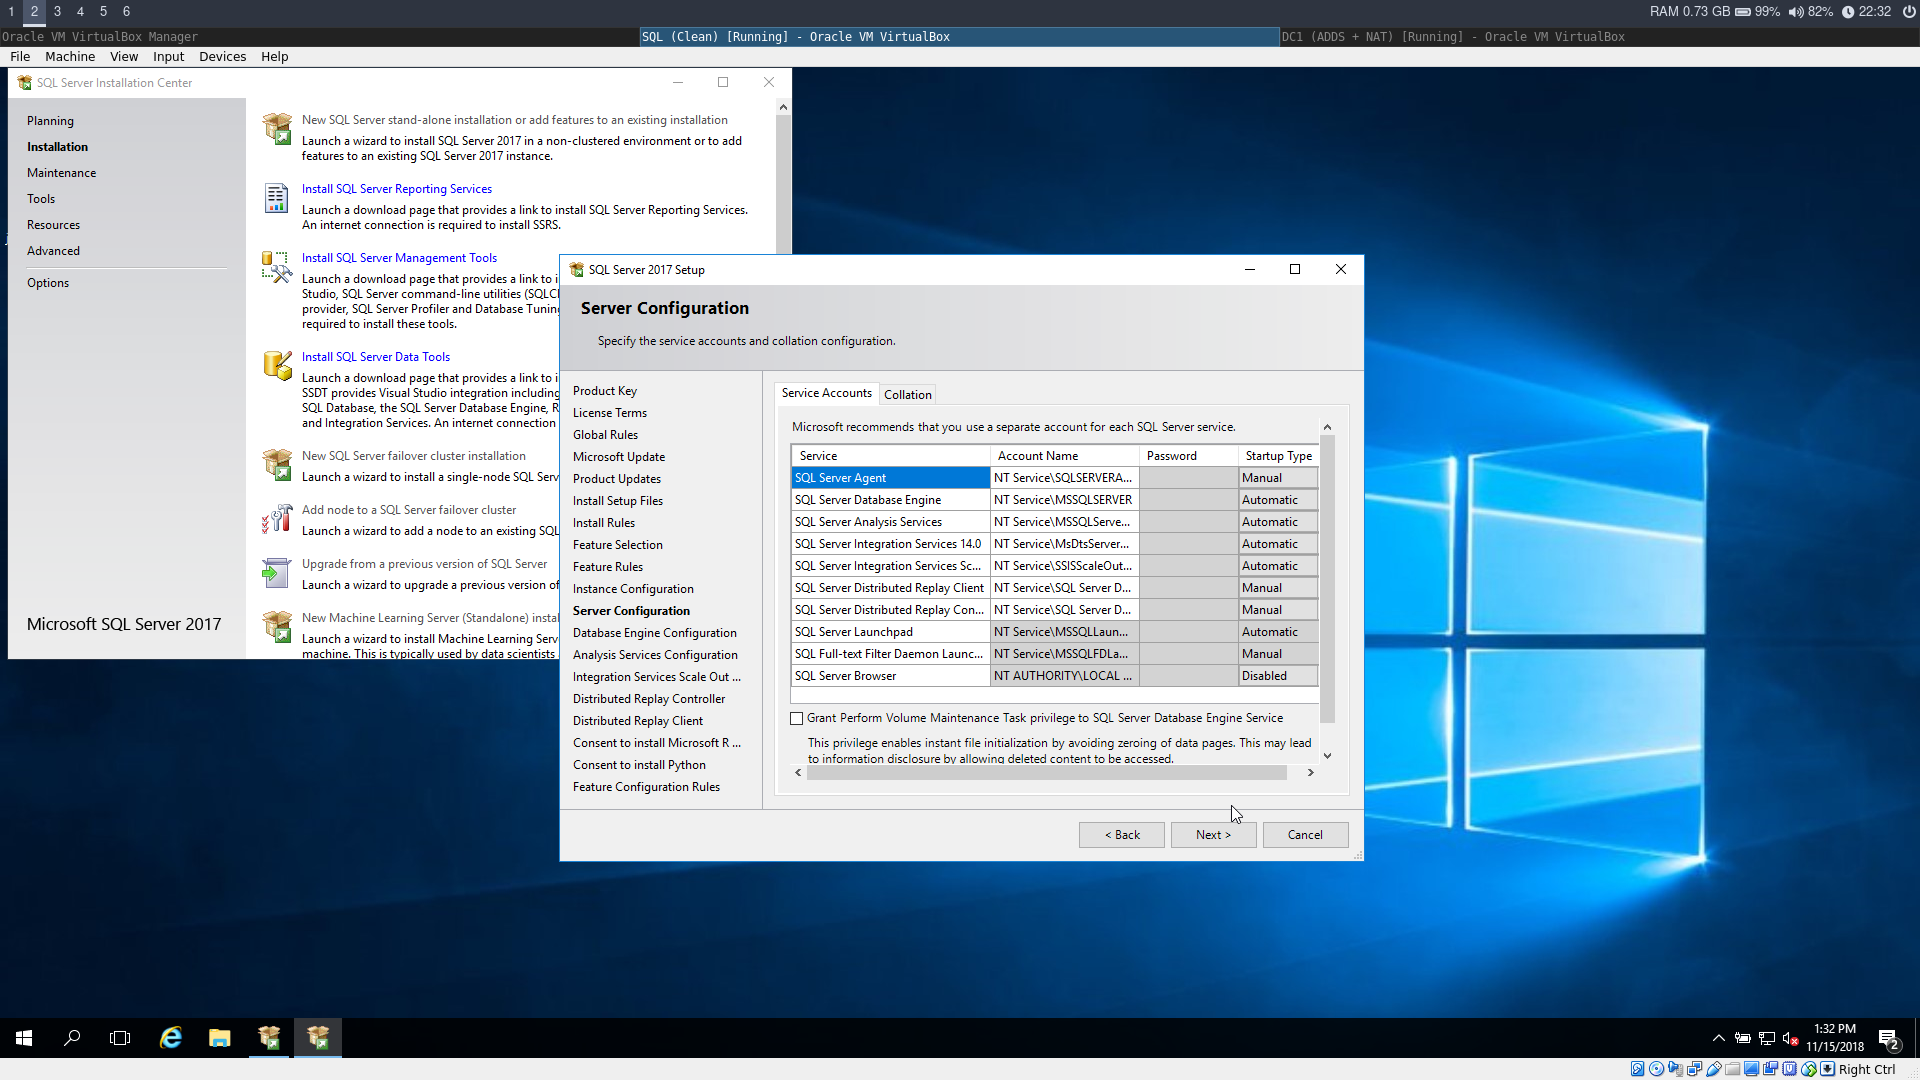
\includegraphics[width=15cm]{Pictures/SQL/1542317574.png}
\end{center}
\begin{center}
	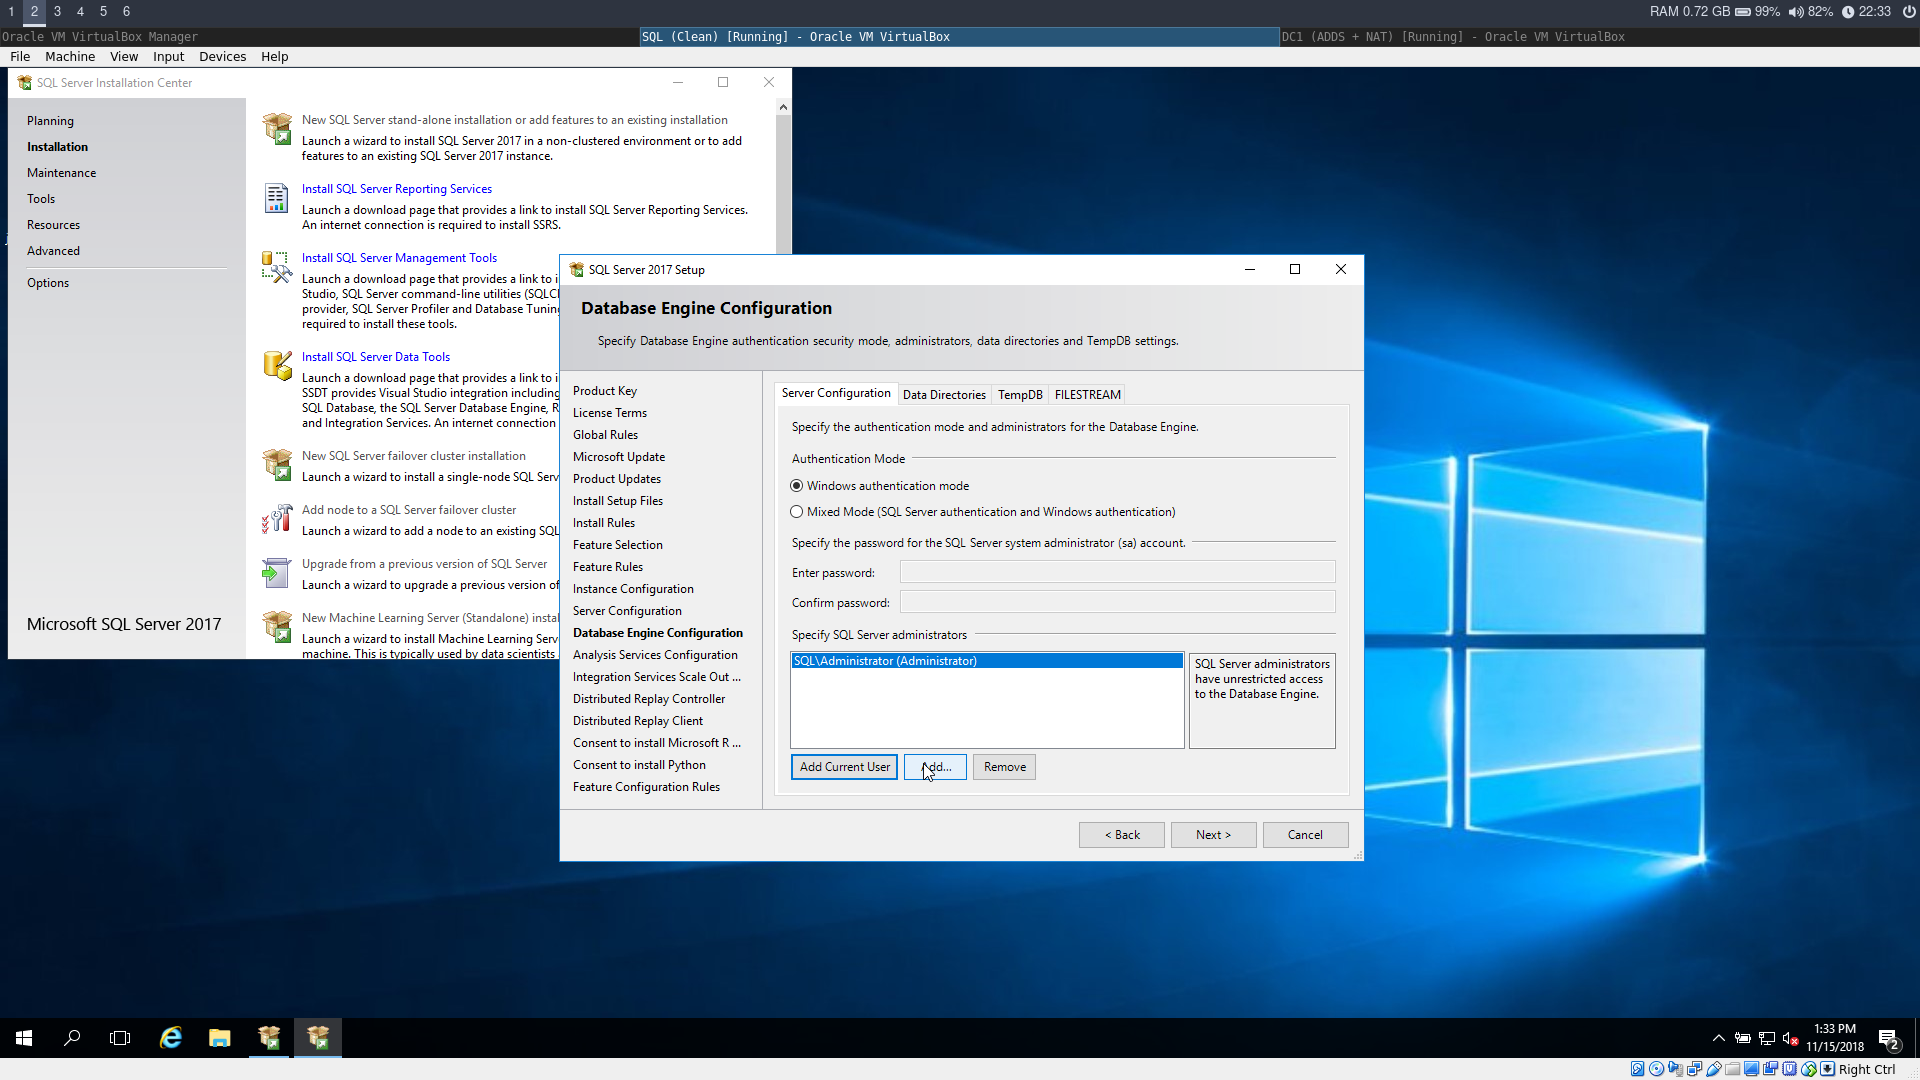
\includegraphics[width=15cm]{Pictures/SQL/1542317584.png}
	
	Voeg de huidige gebruiker toe.
\end{center}
\begin{center}
	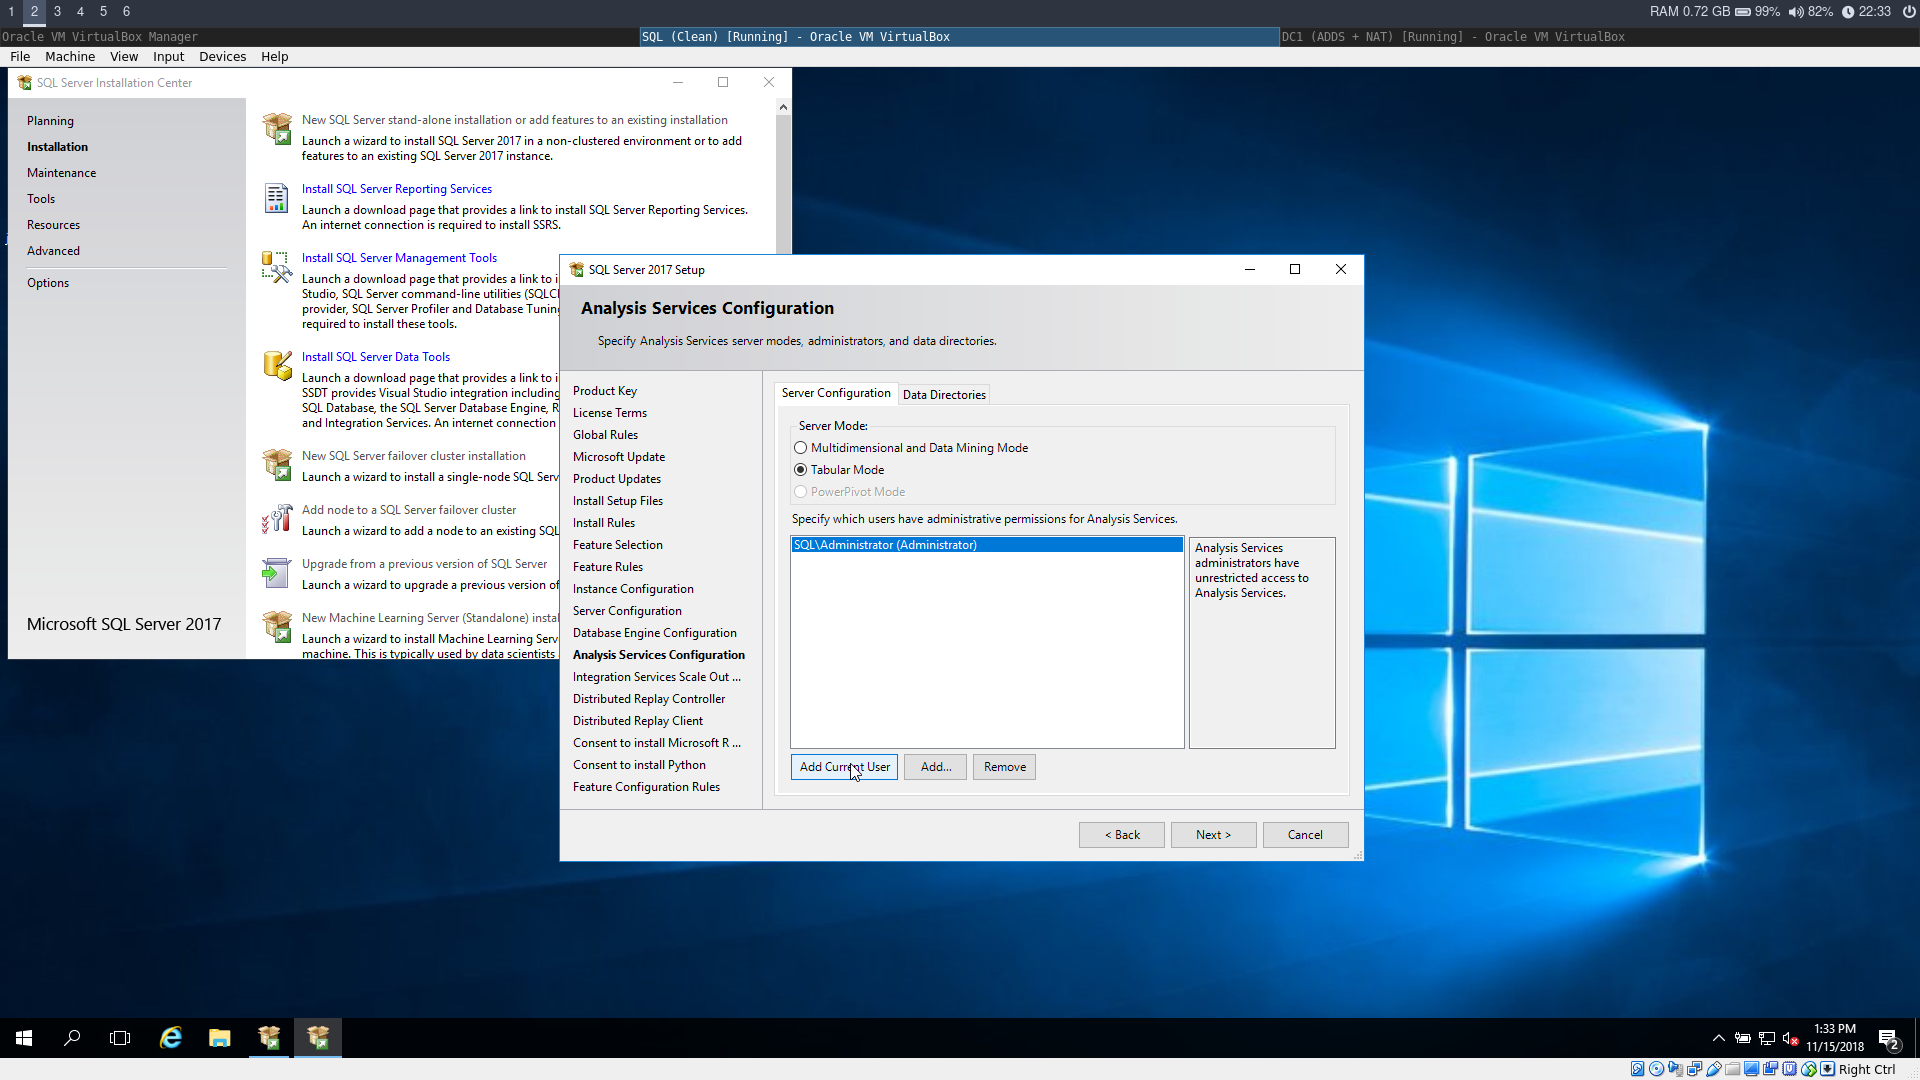
\includegraphics[width=15cm]{Pictures/SQL/1542317590.png}
	
	Voeg de huidige gebruiker toe.
\end{center}
\begin{center}
	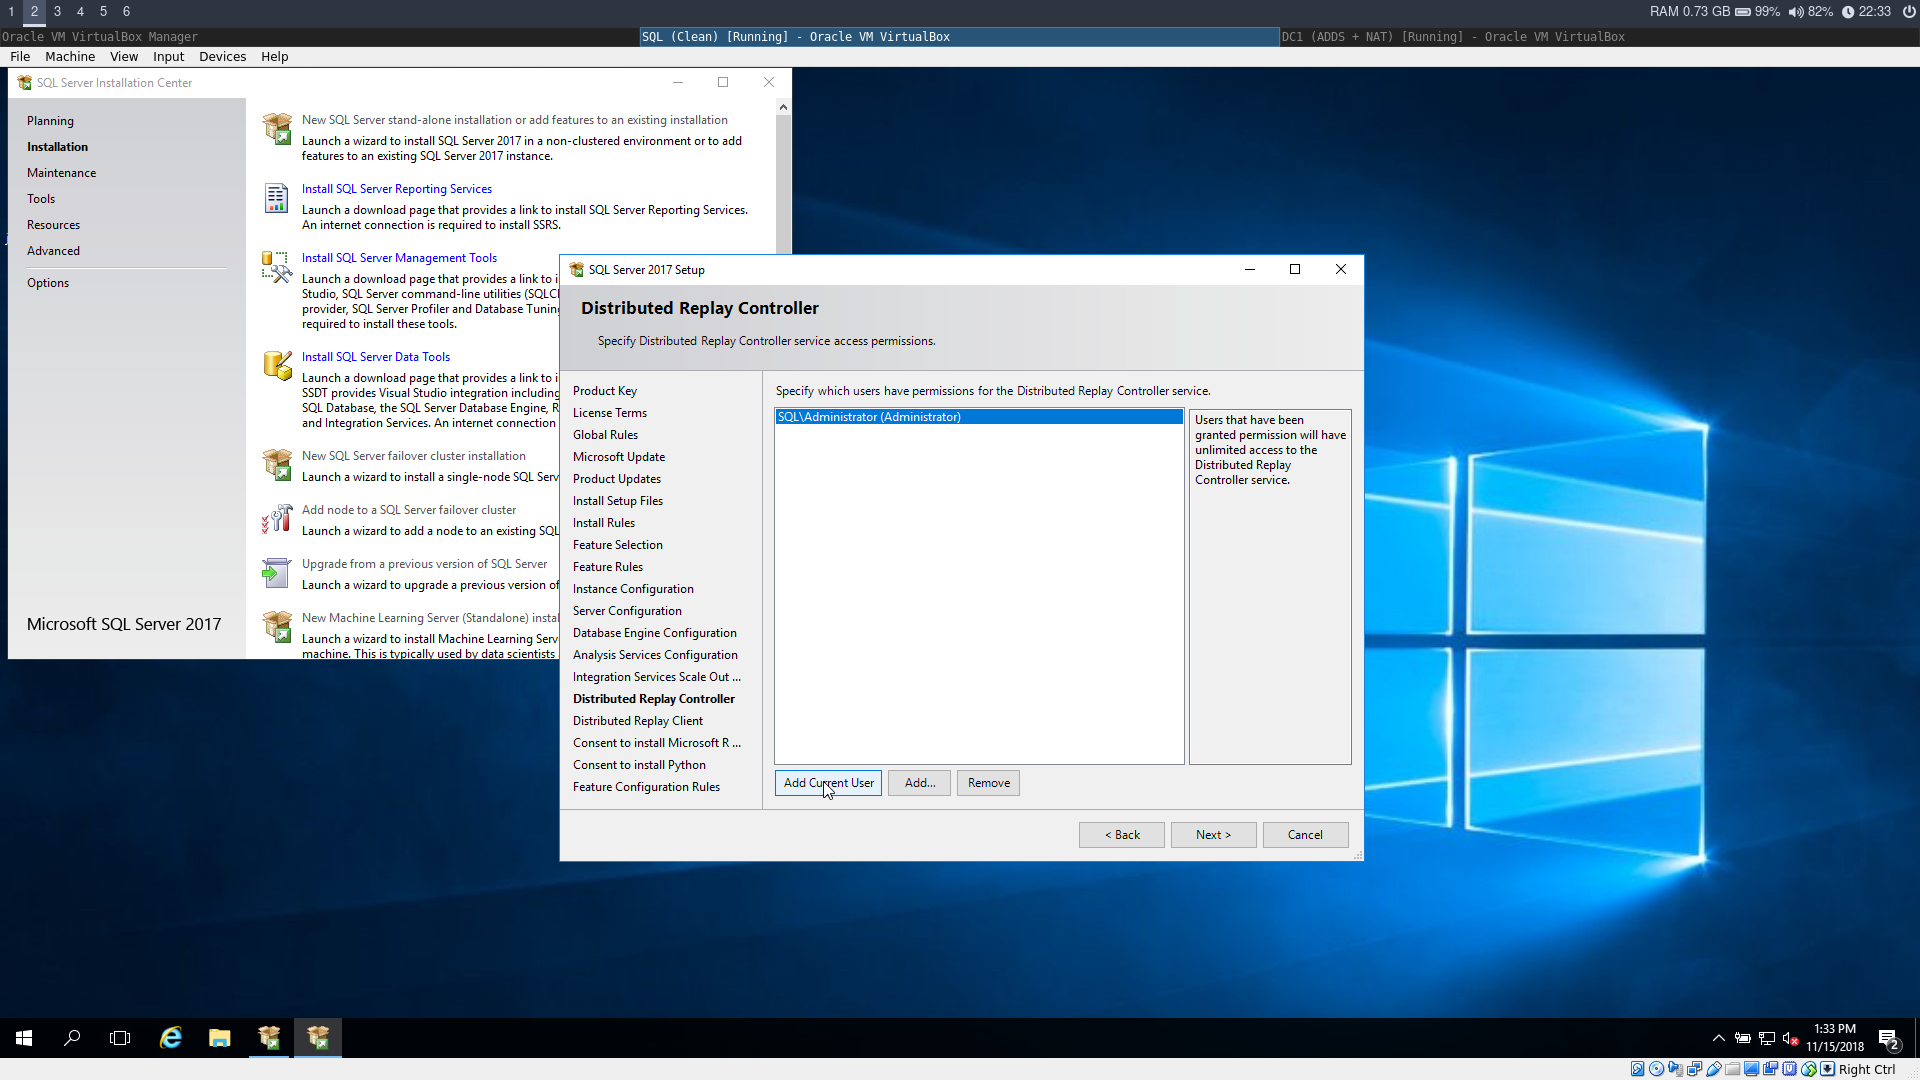
\includegraphics[width=15cm]{Pictures/SQL/1542317599.png}
	
	Voeg de huidige gebruiker toe.
\end{center}
\begin{center}
	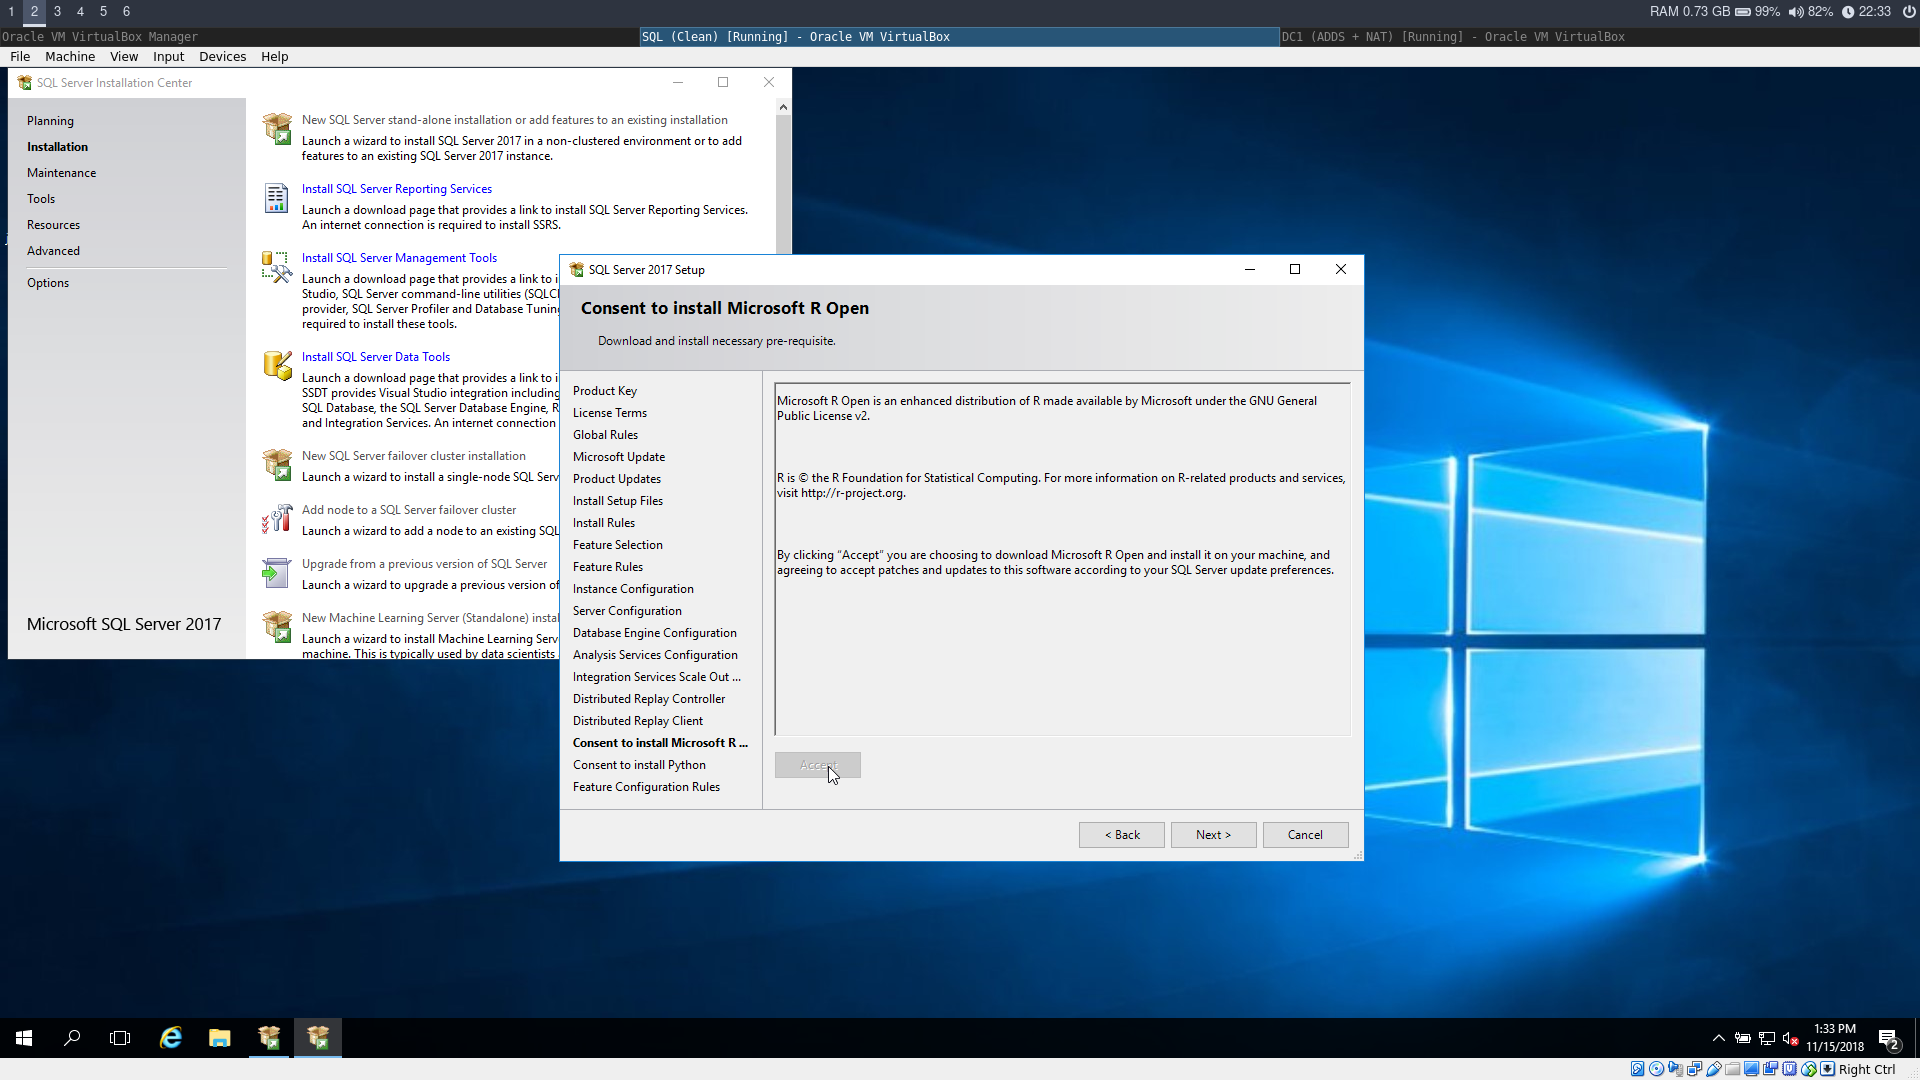
\includegraphics[width=15cm]{Pictures/SQL/1542317621.png}
	
	Ga akkoord met de licentievoorwaarden.
\end{center}
\begin{center}
	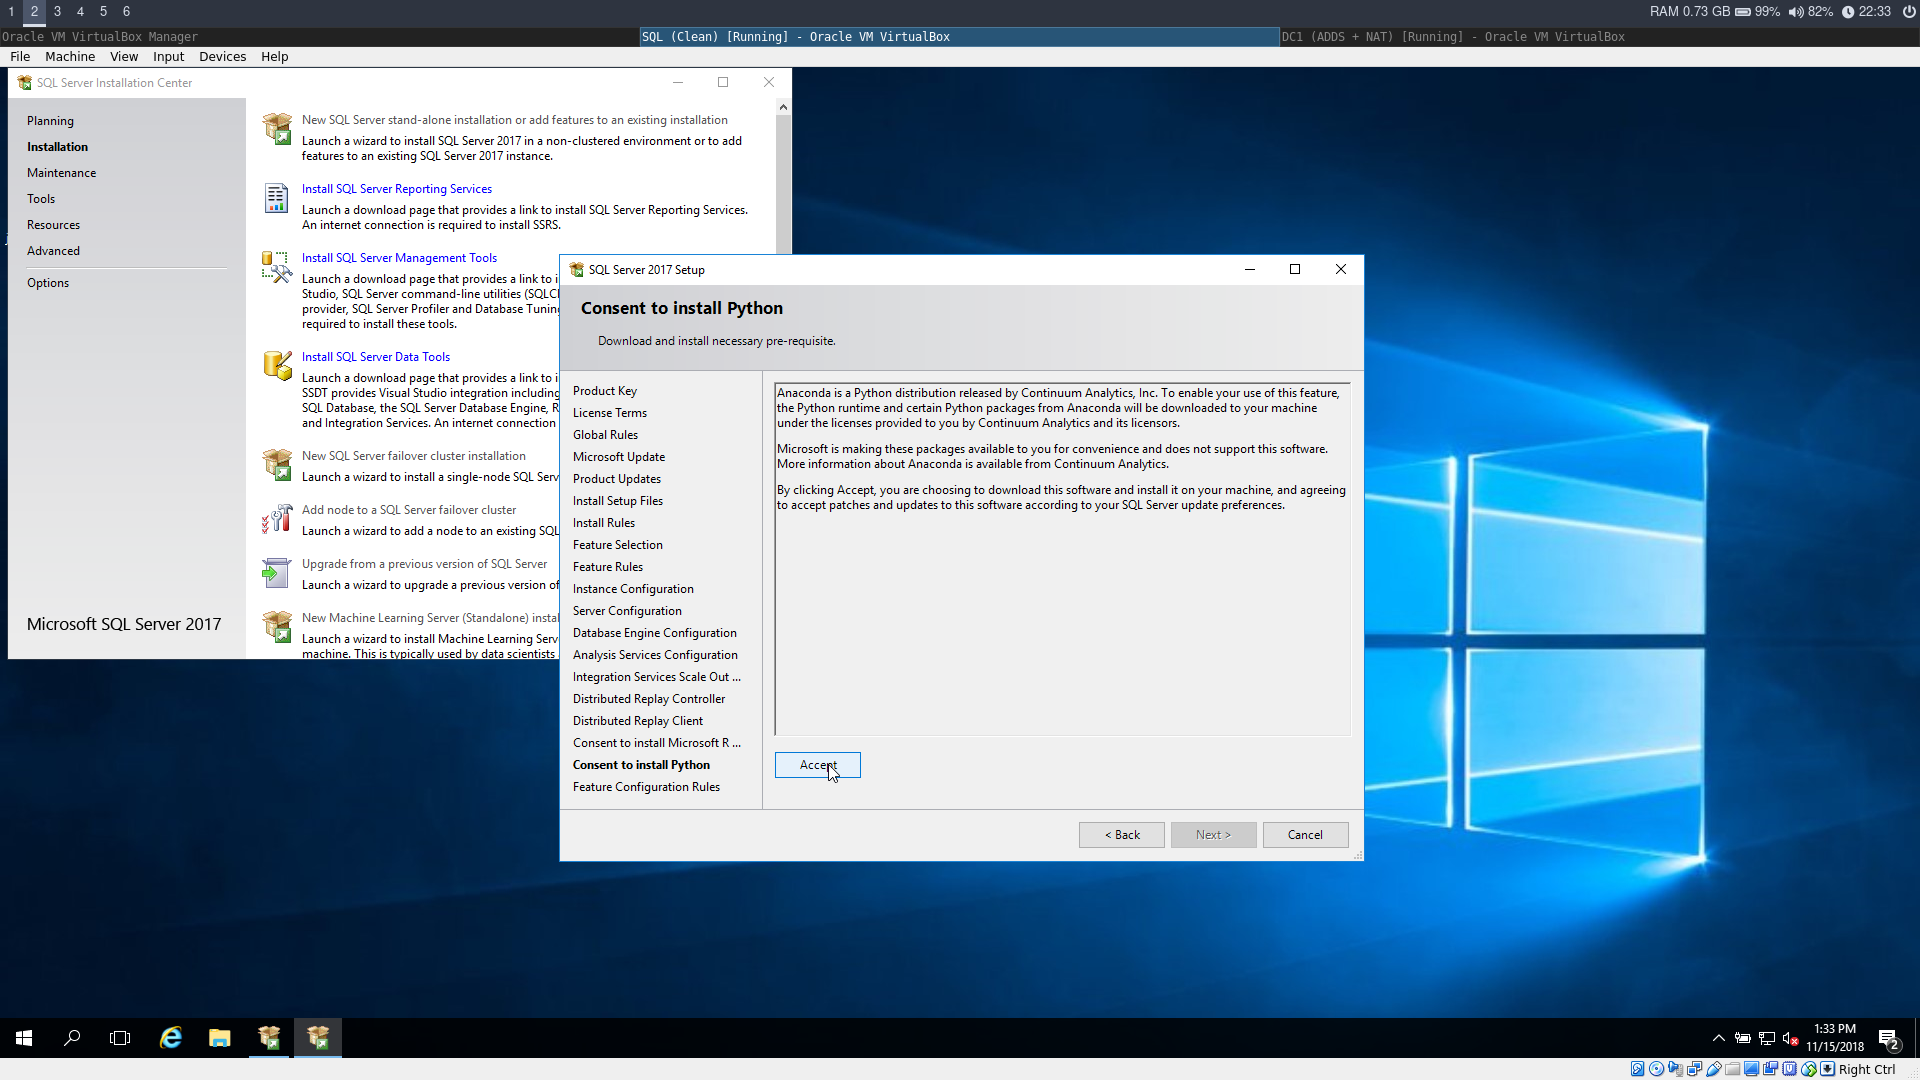
\includegraphics[width=15cm]{Pictures/SQL/1542317631.png}
	
	Ga akkoord met de licentievoorwaarden.
\end{center}
\begin{center}
	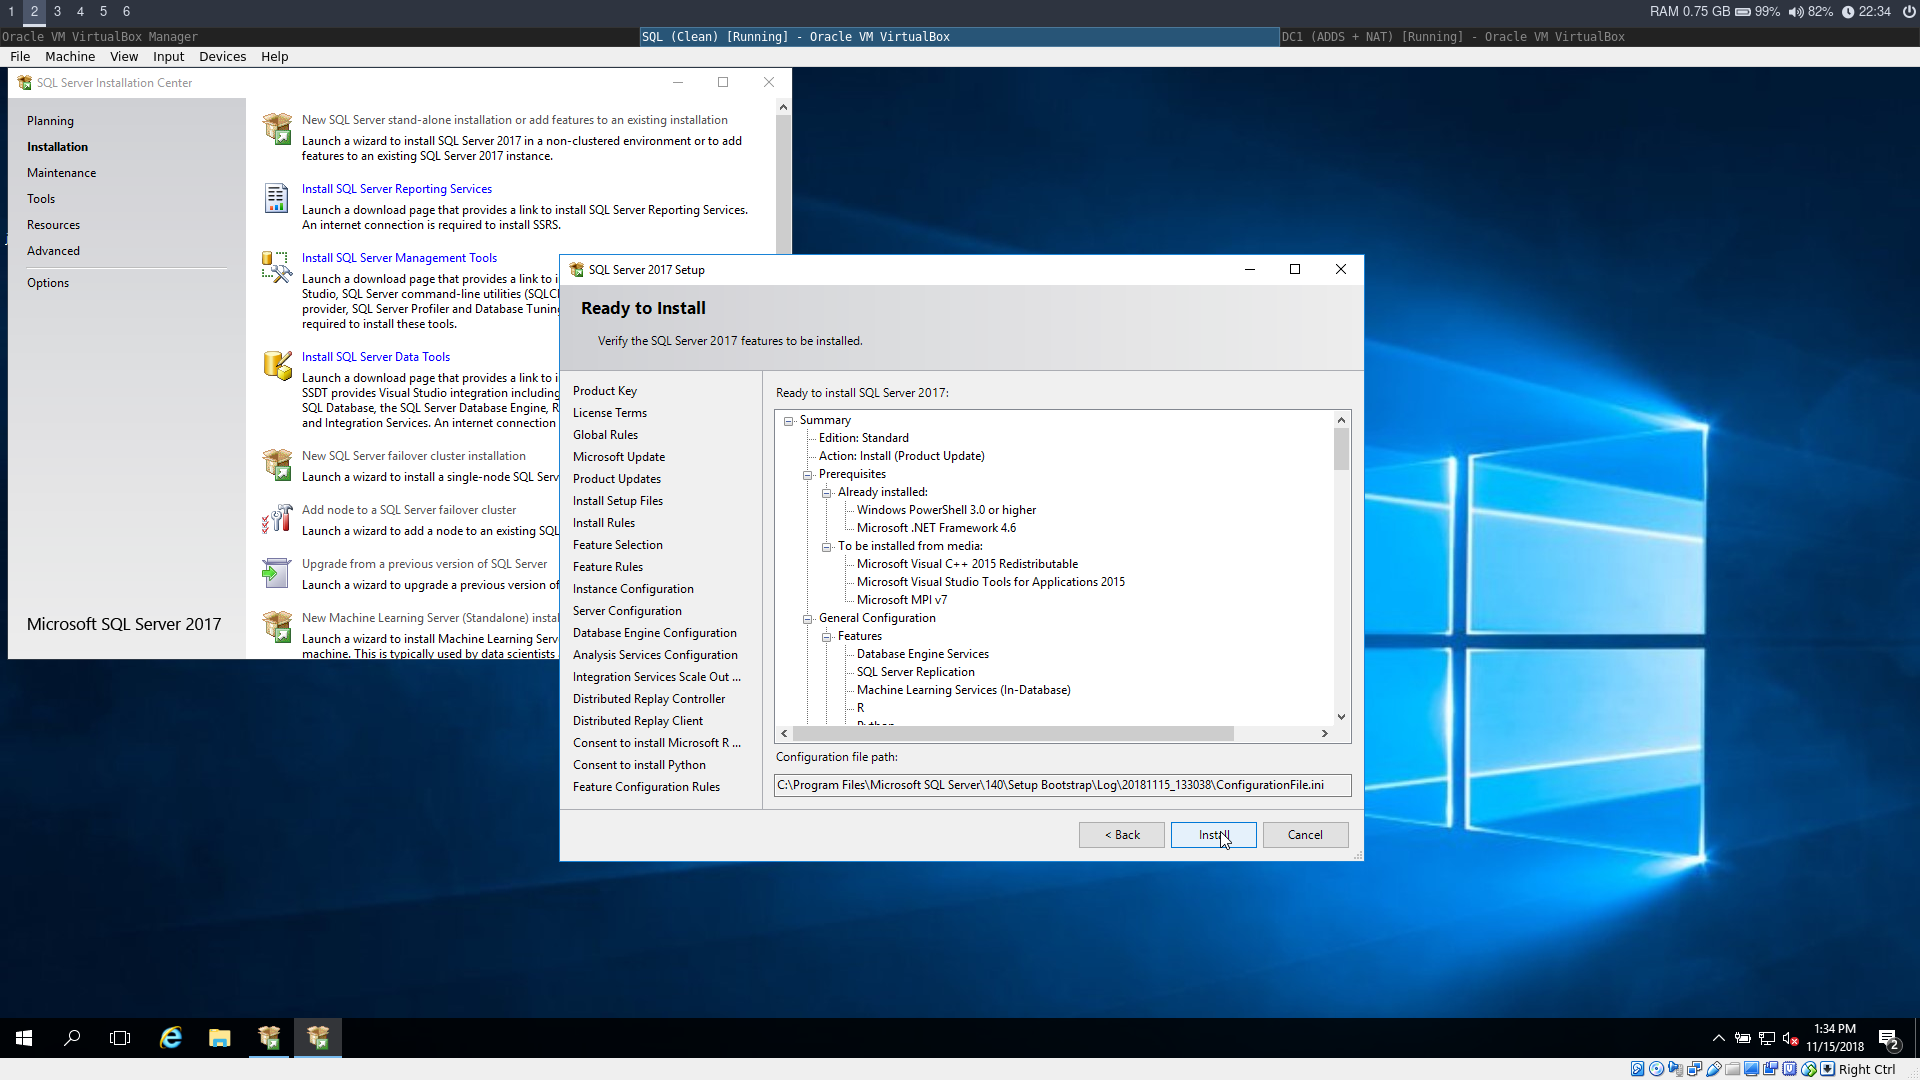
\includegraphics[width=15cm]{Pictures/SQL/1542317645.png}
	
	Start de installatie.
\end{center}
\begin{center}
	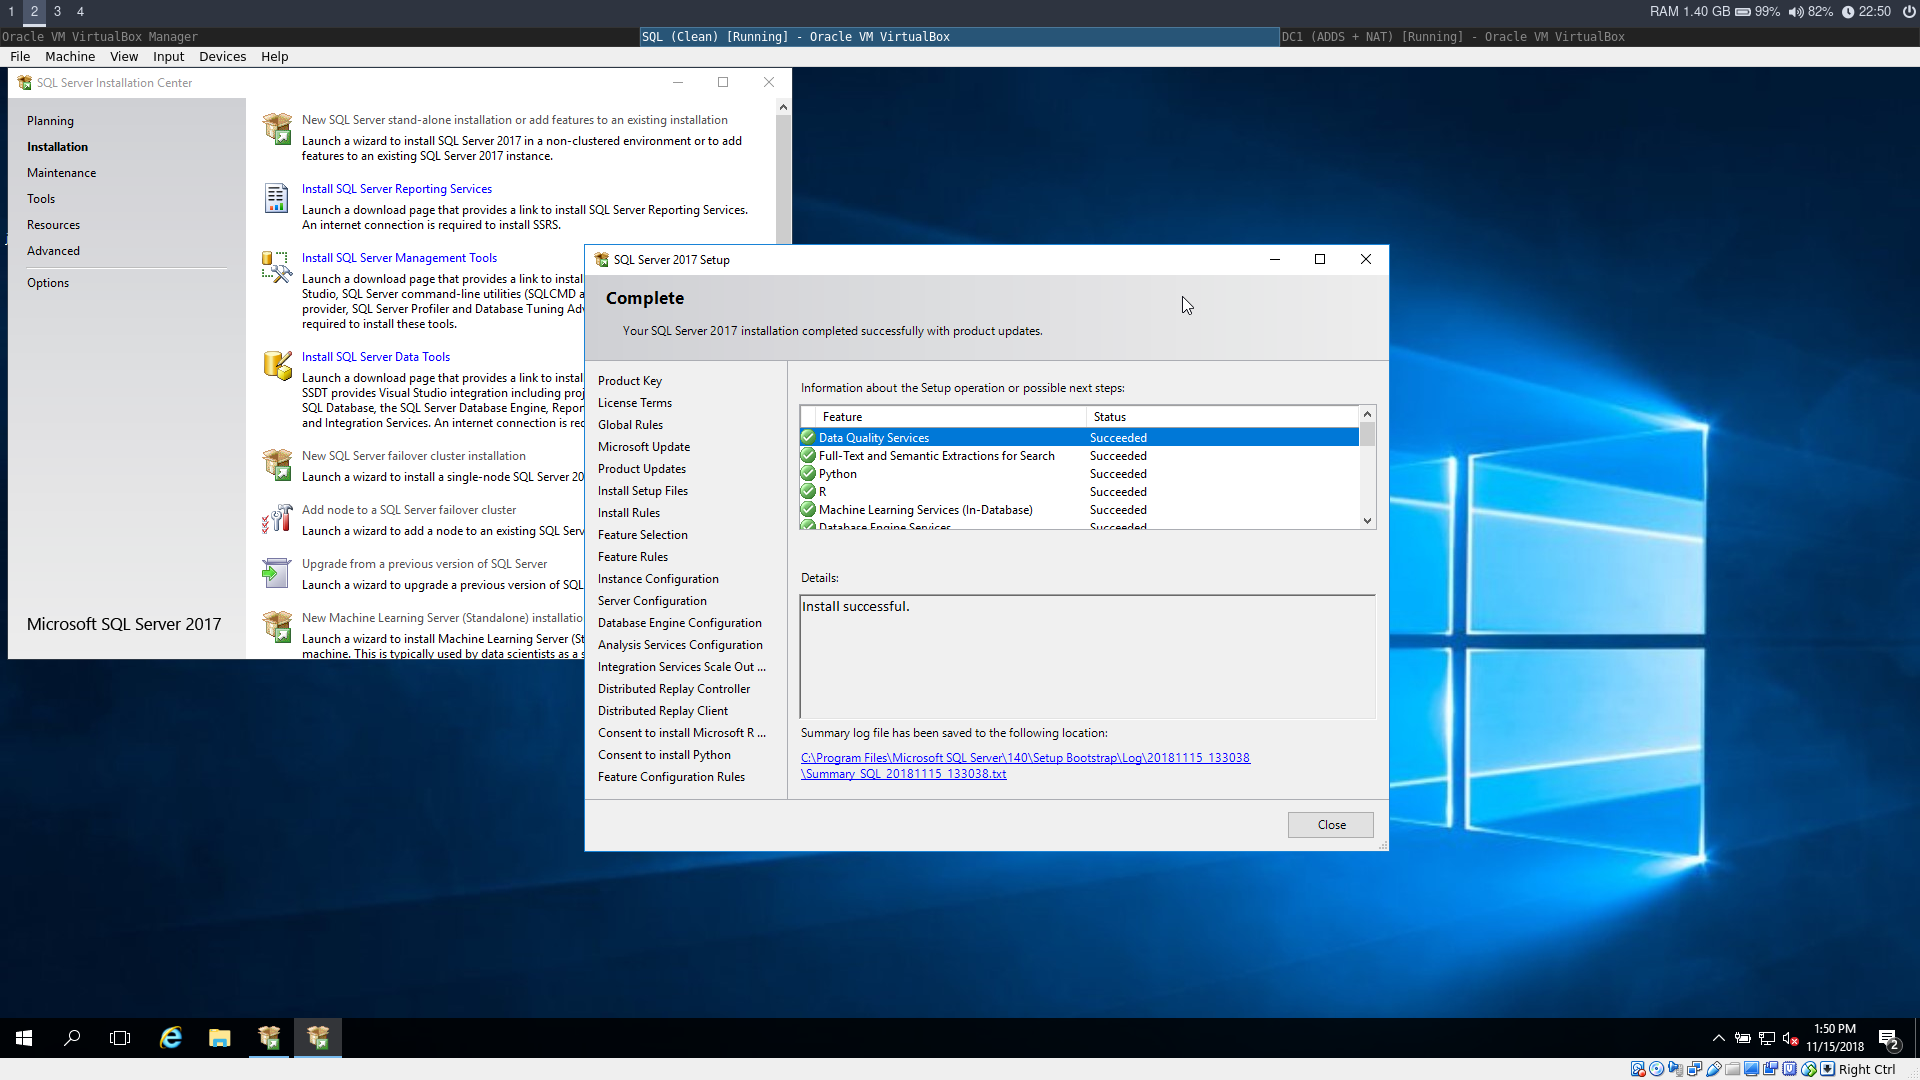
\includegraphics[width=15cm]{Pictures/SQL/1542318646.png}
	
	De installatie is voltooid.
\end{center}
\begin{center}
	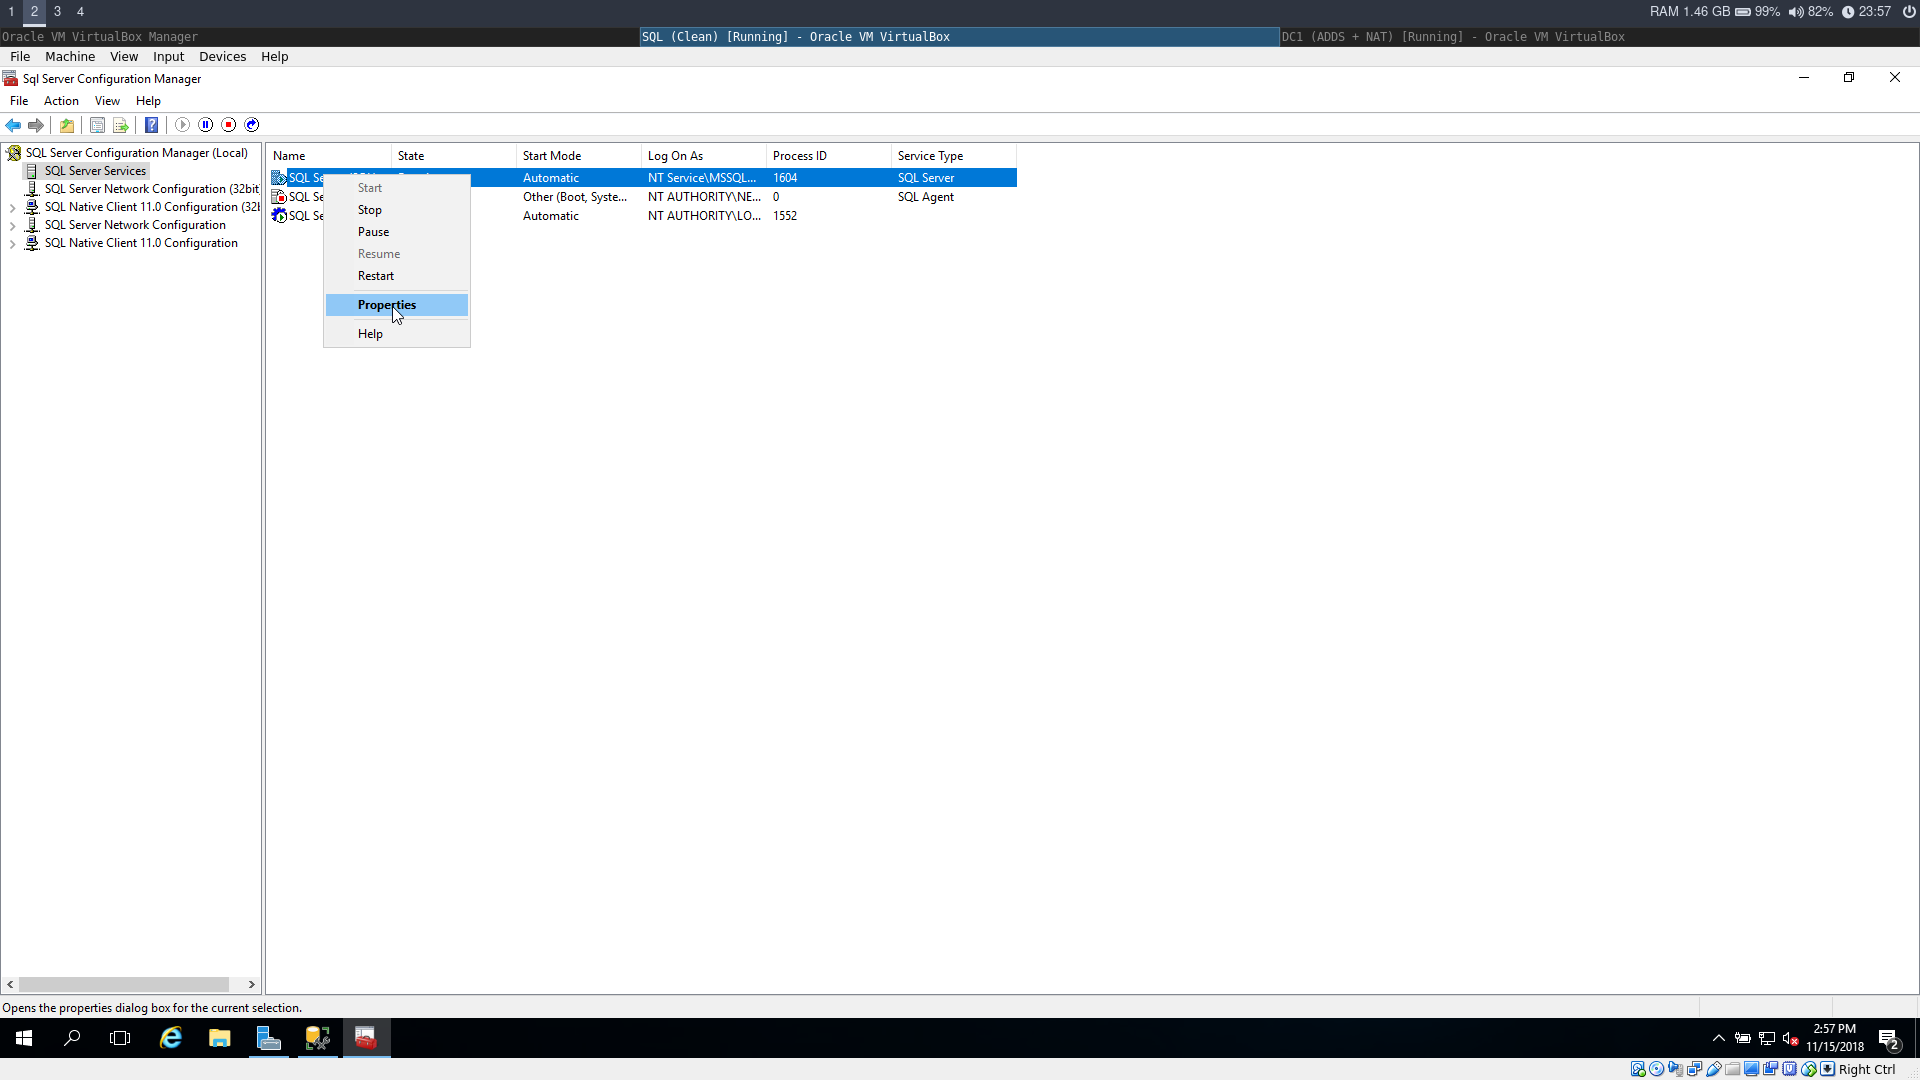
\includegraphics[width=15cm]{Pictures/SQL/1542322667.png}
	
	Open via "SQL Server Configuration Manager" de eigenschappen van de SQL Server.
\end{center}
\begin{center}
	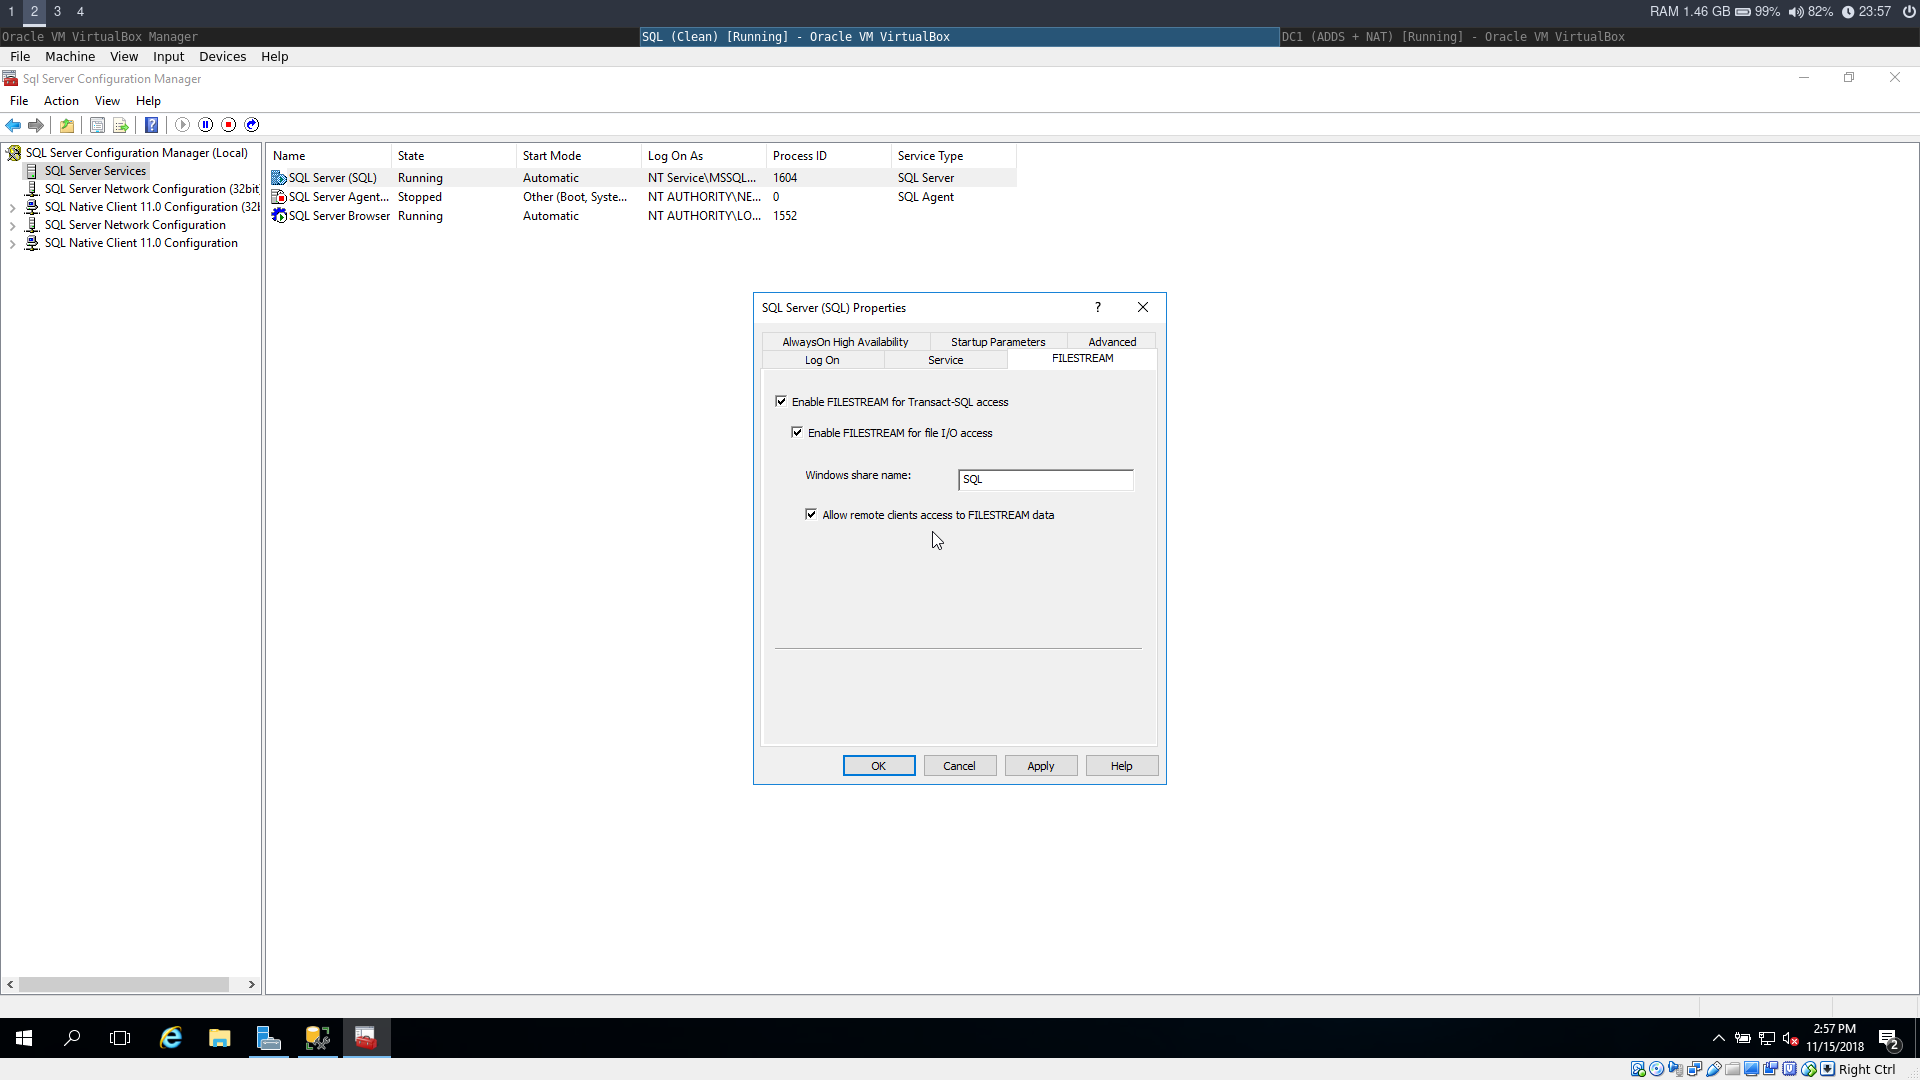
\includegraphics[width=15cm]{Pictures/SQL/1542322673.png}
	
	Vink bij het tablad "FILESTREAM" alles aan.
\end{center}

\clearpage

\section{Connectie vanop DC1}
\begin{center}
	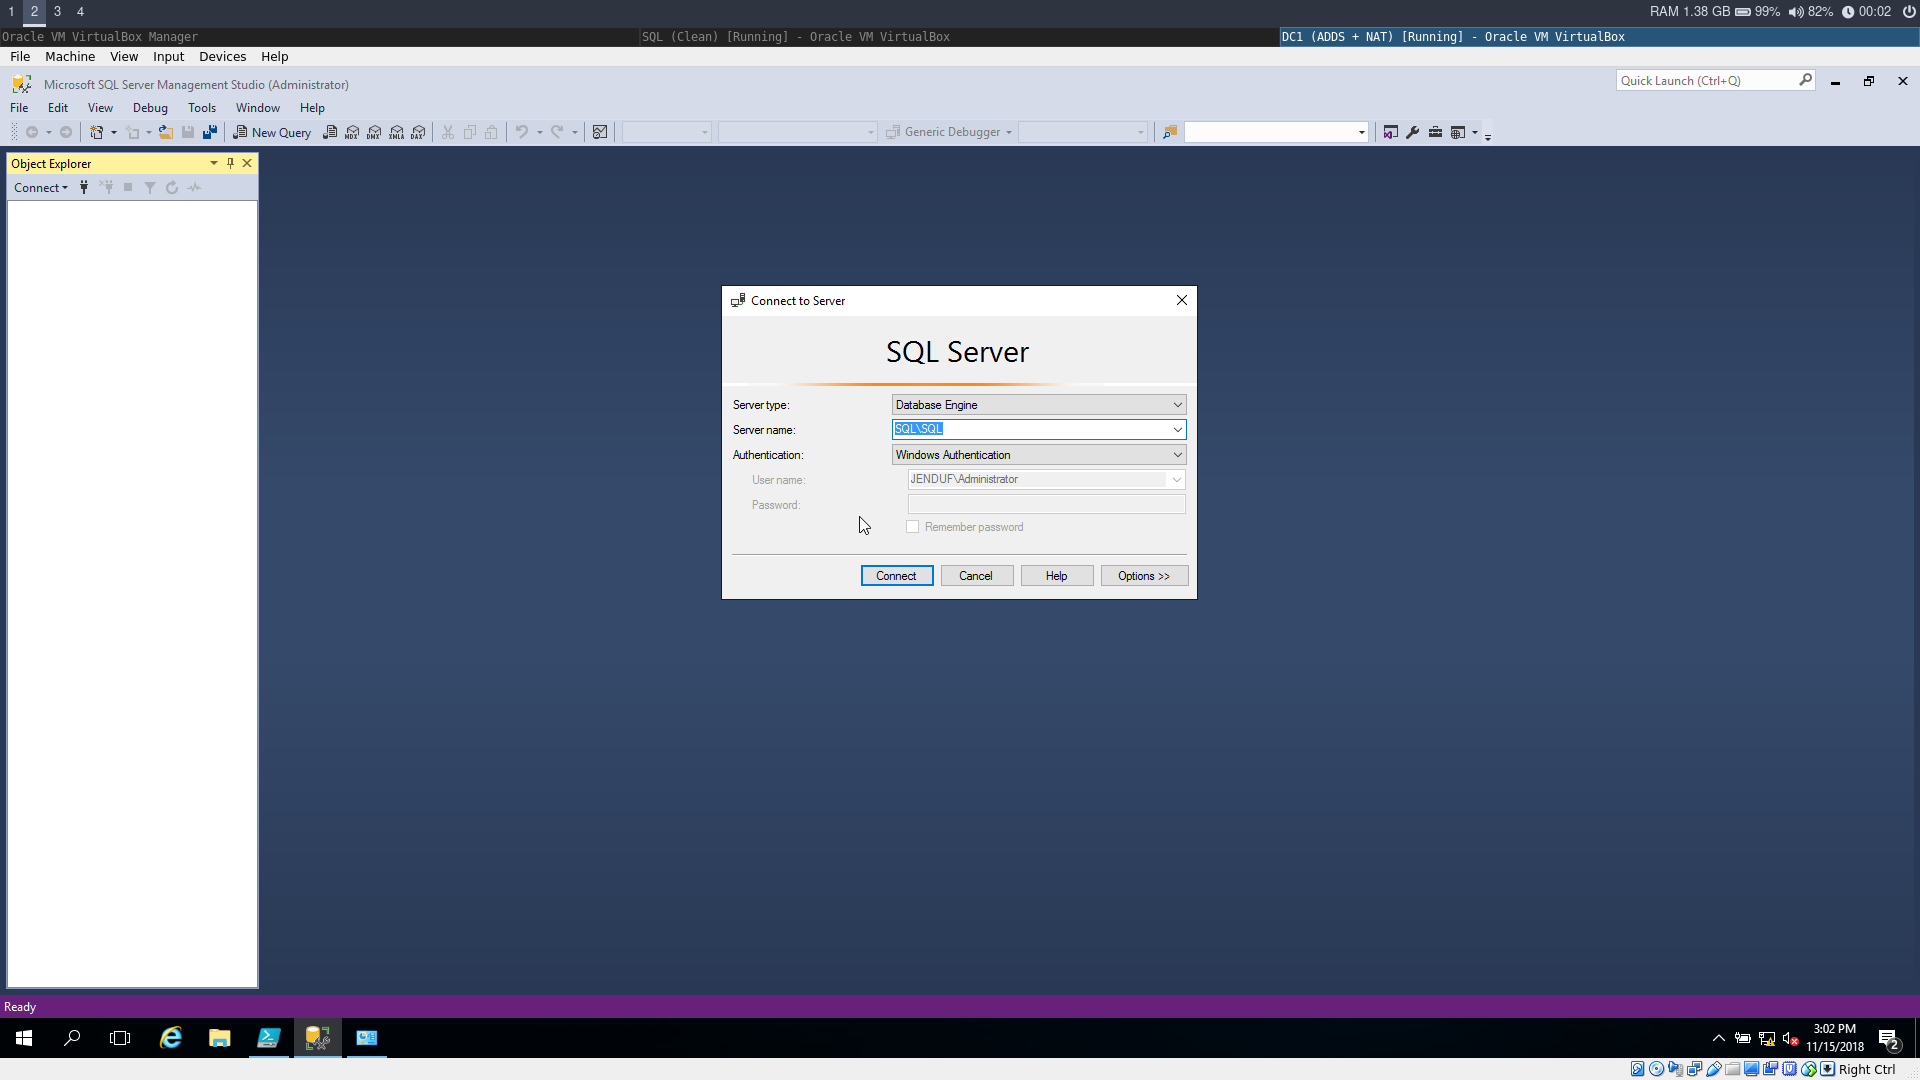
\includegraphics[width=15cm]{Pictures/SQL/1542322958.png}
	
	Connecteer met de aangegeven parameters.
\end{center}
\begin{center}
	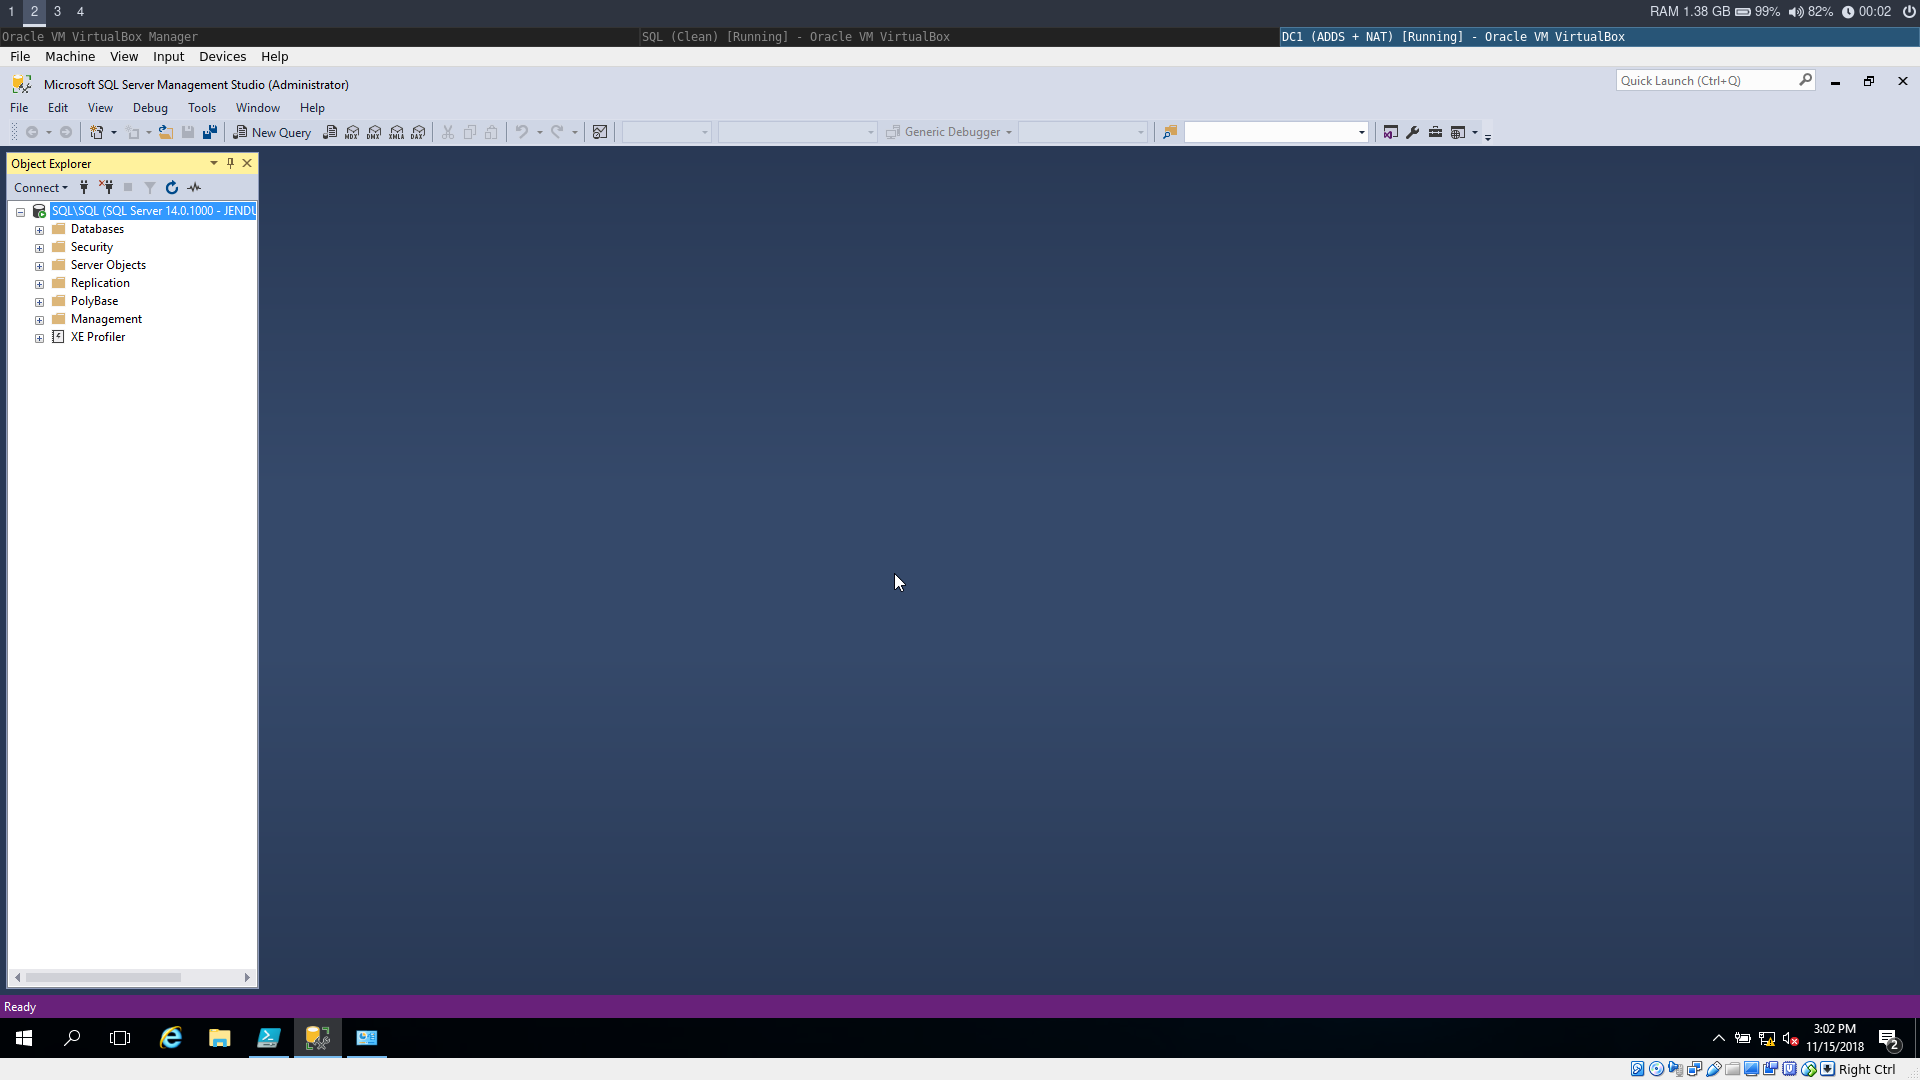
\includegraphics[width=15cm]{Pictures/SQL/1542322961.png}
	
	Bij het zien van dit scherm is de connectie succesvol.
\end{center}

\clearpage
\section{Powershell}

Script 1:

\begin{verbatim}
	#Activeer PS
	Set-ExecutionPolicy Unrestricted
	Function setName{
	Write-Host 'Computernaam wijzigen'
	#Change Name
	Get-WmiObject win32_ComputerSystem
	$ComputerName = Get-WmiObject win32_ComputerSystem
	$name = "SQL"
	$ComputerName.Rename($name)
	}
	
	Function setIP{
	Write-Host 'IP addres geven'
	#IP configuration
	New-NetIPAddress -InterfaceAlias "Ethernet" -IPAddress 192.168.1.3 
	-DefaultGateway 192.168.1.1 -PrefixLength 24
	Set-DnsClientServerAddress -InterfaceAlias "Ethernet" -ServerAddresses 192.168.1.1, 192.18.1.2
	}
	
	Function createDirectories{
	Write-Host 'Directories aanmaken'
	#Directories
	MD 'C:\Program Files\Microsoft SQL Server'
	MD 'C:\Program Files (x86)\Microsoft SQL Server'
	MD 'c:\Program Files (x86)\Microsoft SQL Server\DReplayClient\ResultDir'
	MD 'c:\Program Files (x86)\Microsoft SQL Server\DReplayClient\WorkingDir'
	}
	
	Function NuGet{
	Install-PackageProvider -Name NuGet -MinimumVersion 2.8.5.201 -Force
	}
	
	Function ServerManager {
	Import-Module ServerManager
	}
	
	setName
	setIP
	createDirectories
	NuGet
	ServerManager
	Restart-Computer
	
	
\end{verbatim}

Script 2:

\begin{verbatim}
Function Firewall{
Write-Host 'Firewall Config'
Set-NetFirewallProfile -Profile Domain,Public,Private -Enabled False
Write-Host 'Firewall Rule Port 1433'
New-NetFirewallRule -DisplayName "MSSQL ENGINE TCP" -Direction Inbound 
-LocalPort 1433 -Protocol TCP -Action Allow
}

Function JoinDomain{
Write-Host 'Trying to join domain jenduf.gent'
$DomainName = "jenduf.gent"
$SafeModeAdministratorPassword = "Admin2018" | ConvertTo-SecureString -AsPlainText -Force
$domain = "jensduf"
$joindomainuser = "Administrator"
$credential = New-Object System.Management.Automation.PSCredential
($joindomainuser,$SafeModeAdministratorPassword)
Add-Computer -DomainName $DomainName -Credential $credential
}

JoinDomain
Firewall
Restart-Computer
\end{verbatim}

Script 3:

\begin{verbatim}
Function SQL{
echo "Downloading SQL..."
cd C:/
wget "https://download.microsoft.com/download/5/E/9/5E9B18CC-8FD5-467E-B5BF-BADE39C51F73/
SQLServer2017-SSEI-Expr.exe" -OutFile SQLServer2017-SSEI.exe
Start-Process -FilePath ./SQLServer2017-SSEI.exe -ArgumentList "/action=download 
/quiet /enu /MediaPath=C:/" -wait
Remove-Item ./SQLServer2017-SSEI.exe
Start-Process -FilePath C:/SQLEXPR_x64_ENU.exe -WorkingDirectory C:/ /q -wait
Write-Host 'SQL Installeren'
Start-Process -FilePath C:/SQLEXPR_x64_ENU/SETUP.EXE -ArgumentList "/Q /Action=install 
/IAcceptSQLServerLicenseTerms /FEATURES=SQL,Tools /TCPENABLED=1 /SECURITYMODE=`"SQL`" 
/SQLSYSADMINACCOUNTS=`"BUILTIN\Administrators`" /INSTANCENAME=`"SQL`" /INSTANCEID=`"SQL`" 
/SAPWD=`"@Admin2018`"" -wait

}

Function SSMS{
Write-Host 'SQL Managemnt Studio Installeren'
cd C:/
wget "https://go.microsoft.com/fwlink/?linkid=858904" -OutFile SSMS-Setup-ENU.exe
Start-Process -FilePath "C:\SSMS-Setup-ENU.exe" -ArgumentList '/s' -Wait -PassThru
}

SQL
SSMS
Restart-Computer

\end{verbatim}

\end{document}